% ****** Start of file aipsamp.tex ******
%
%   This file is part of the AIP files in the AIP distribution for REVTeX 4.
%   Version 4.1 of REVTeX, October 2009
%
%   Copyright (c) 2009 American Institute of Physics.
%
%   See the AIP README file for restrictions and more information.
%
% TeX'ing this file requires that you have AMS-LaTeX 2.0 installed
% as well as the rest of the prerequisites for REVTeX 4.1
% 
% It also requires running BibTeX. The commands are as follows:
%
%  1)  latex  aipsamp
%  2)  bibtex aipsamp
%  3)  latex  aipsamp
%  4)  latex  aipsamp
%
% Use this file as a source of example code for your aip document.
% Use the file aiptemplate.tex as a template for your document.
\documentclass[%
 aip,
% jmp,
% bmf,
% sd,
% rsi,
 amsmath,amssymb,
%preprint,%
 reprint,%
%author-year,%
%author-numerical,%
% Conference Proceedings
]{revtex4-1}

\usepackage{graphicx}% Include figure files
\usepackage{dcolumn}% Align table columns on decimal point
\usepackage{bm}% bold math
\usepackage{subcaption}
\usepackage{booktabs}
%\usepackage[mathlines]{lineno}% Enable numbering of text and display math
%\linenumbers\relax % Commence numbering lines

\usepackage[utf8]{inputenc}
\usepackage[T1]{fontenc}
\usepackage{mathptmx}
\usepackage{etoolbox}

% ADDED FOR DRAFTING (TODO)
\usepackage{enumitem}
\setlist[itemize]{noitemsep} 

% Custom additions
\newcommand{\gene}[1]{\rmfamily\textsc{Gene}#1}

%% Apr 2021: AIP requests that the corresponding 
%% email to be moved after the affiliations
\makeatletter
\def\@email#1#2{%
 \endgroup
 \patchcmd{\titleblock@produce}
  {\frontmatter@RRAPformat}
  {\frontmatter@RRAPformat{\produce@RRAP{*#1\href{mailto:#2}{#2}}}\frontmatter@RRAPformat}
  {}{}
}%
\makeatother
\begin{document}

\preprint{AIP/123-QED}

\title{Radiation Temperature Fluctuation Measurements in Optically Semi-transparent Helically Symmetric Experiment Plasmas}
% Force line breaks with \\

\author{L. Singh}
 \affiliation{University of Wisconsin--Madison, Madison, WI, USA}%Lines break automatically or can be forced with \\
 
\author{G.W. Held}%
 \affiliation{University of Wisconsin--Madison, Madison, WI, USA}%

\author{G.M. Weir}
 \affiliation{Max Planck Institute for Plasma Physics, Greifswald, DE}%

\author{B.J. Faber}
 \affiliation{University of Wisconsin--Madison, Madison, WI, USA}%

\author{K.M. Likin}
 \affiliation{University of Wisconsin--Madison, Madison, WI, USA}%

\author{H.O. Miller}
 \affiliation{University of Wisconsin--Madison, Madison, WI, USA}%

\author{M. Wezeman}
 \affiliation{Eindhoven University of Technology, Eindhoven, NL}%

\author{A.M.A Jacobs}
\affiliation{Fontys University of Applied Sciences, Eindhoven, NL}%

\author{M.J. Pueschel}
 \affiliation{Dutch Institute for Fundamental Energy Research, Eindhoven, NL}%

\author{C.C. Hegna}
 \affiliation{University of Wisconsin--Madison, Madison, WI, USA}
 \affiliation{Type One Energy Group}

\author{B. Geiger}
 \affiliation{University of Wisconsin--Madison, Madison, WI, USA}%

\date{\today}% It is always \today, today,
             %  but any date may be explicitly specified

\begin{abstract}
An article usually includes an abstract, a concise summary of the work
covered at length in the main body of the article. It is used for
secondary publications and for information retrieval purposes. 
\end{abstract}

\maketitle

\section{\label{sec:intro}Introduction}

\begin{itemize}
    \item Motivation 
    \begin{itemize}
        \item Neoclassical transport reduced w.r.t. classical stellarators with QHS in HSX
        \item Anomalous transport dominant, as in a tokamak
        \item Anomalous component commonly attributed to fluctuation-induced turbulent transport associated with plasma microturbulence 
    \end{itemize}
    
    \item Previous fluctuation measurements performed at HSX
    \begin{itemize}
        \item Direct measurements of turbulent transport are challenging, involving simultaneous measurement of fluctuations in multiple equilibrium quantities. Examples in stellarators include (refs), which employ advanced diagnostics that are infeasible due to spatial constraints in HSX. More routine are measurements of a single fluctuating field, which have been performed previously at HSX.
        \item Previous core measurements (reflectometer, ref: Jason, Konstantin; interferometer, ref: Deng)
        \item Interpretation of measurements consistent gyrokinetic simulations of plasma turbulences (many refs)
    \end{itemize}

    \item More on simulations of turbulence, TEM, ETG, hinting at temperature gradient drive. 

    \item What we're doing in this paper: temperature fluctuation measurements with correlation ECE in semi-transparent plasma.
    \begin{itemize}
        \item 
    \end{itemize}
    
\end{itemize}

\section{\label{sec:methods}Analysis and Interpretation of CECE in HSX}
% Despite low optical depth, previously shown that the emission can be localized (HFS, thermal, high density)

% We can't used ECE due to noise fluctuations --> CECE

% Sensitivity, amplitude and wavenumber space

A CECE diagnostic measures temperature fluctuation measurements in the HSX stellarator.  Due to relatively low electron pressure and corresponding low reabsorption of emitted radiation in the core plasma, the measured radiation temperature fluctuations contain an electron temperature and density fluctuation component. intensity of emission measured by the ECE radiometer may not be directly proportional to the electron temperature $T_e$. As such, it is more appropriate to directly consider the radiation temperature $T_r$ as the fundamental quantity in the context of ECE measurements in the HSX stellarator. It has previously been shown that under specific experimental conditions, radial profiles of $T_r$ measured via ECE are consistent with $T_e$ as measured by Thomson scattering \cite{weir-thesis}. Still, fluctuations in radiation temperature $\delta T_r/T_r$ are a more sensitive quantity and are modified by density fluctuations $\delta n/n$. 

% Modeling of the ECE emissivity is shown in Section \ref{sec:hsx_rad_transport} to determine the localization of CECE measurements. 

% The difference between $\delta T_r/T_r$ and $\delta T_e/T_e$ is clarified in Section \ref{sec:sys_error} where the systematic error in interpreting $\delta T_r/T_r$  as $\delta T_e/T_e$  is estimated in HSX. Finally, a description of the correlation ECE data analysis is provided in Section \ref{sec:cece_anal}.

\begin{figure*}[!htbp]
\centering
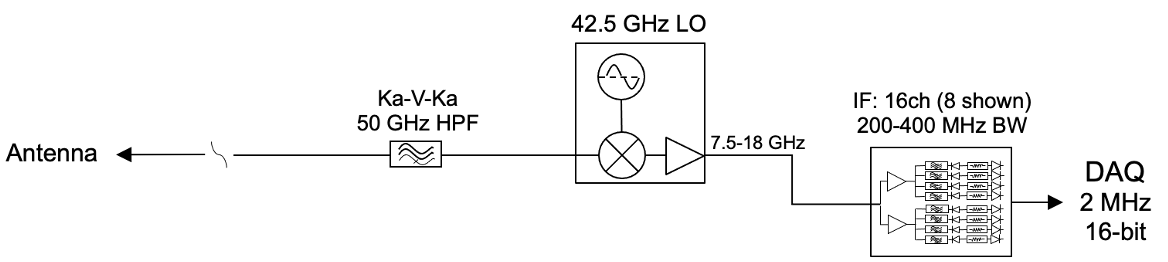
\includegraphics[width=0.95\textwidth]{Figures/hsx_cece.png}
\caption{Radiometer block diagram for the HSX ECE diagnostic. The radiometer back-end is comprised of 16 spectral channels. }
\label{fig:radiometer}
\end{figure*}

% Basics of diagnostic
% TODO: combine this with resolution (i.e. connect power radius with average radial extent)
A block diagram for the ECE diagnostic used for operation with on-axis field strength $B=1$\,T is shown in Fig.\ \ref{fig:radiometer}. The antenna refers to the combination of the ellipsoidal mirror coupled with a pyramidal horn. The transmission line consists primarily of Ka band waveguide, but a segment of V band waveguide (which has a lower frequency cutoff of 50\,GHz) acts as a high pass filter, filtering out the lower side band and stray gyrotron radiation. A 42.5\,GHz local oscillator signal mixes signals down to the IF range 7.5-18\,GHz. The mixed signal is amplified and then split into 16 channels using 2-way and 8-way power dividers, with amplification following each power division. The signal is band-pass filtered with an intermediate frequency (IF) filter, detected, low-pass filtered, and again amplified before being sent to a data acquisition device. The exact relationship between the intermediate frequency and measurement localization is dictated by the shape of the ECE emissivity, which depends on $n$ and $T_e$ and $B$. The ECE signal level is proportional to $B_\mathrm{IF}$ because a wider band admits radiation from a larger plasma region.

%%%%%%%%%%%%%%%%%%%%%%%%%%%%%%%%%%%%%%%%%%%%%%%%%%%%%%%%%%%%%%%%%%%%%%%%%%%%%%%%%%%%%%%%%%%%%%%%%%%%%%%%%%%%%%%%%%%%%%
% Below are the wavenumber sensitivies, which are relevant for synthetic diagnostic filtering and interpreting physics of measurements
%%%%%%%%%%%%%%%%%%%%%%%%%%%%%%%%%%%%%%%%%%%%%%%%%%%%%%%%%%%%%%%%%%%%%%%%%%%%%%%%%%%%%%%%%%%%%%%%%%%%%%%%%%%%%%%%%%%%%%

% Power radius
 The beam power radius $b \approx 1.5$\,cm, defined as the $1/e^2$ radius of the beam power has been previously modeled by propagating a Gaussian beam out the throat of the horn antenna, invoking optical reciprocity \cite{weir-thesis}. The corresponding maximum resolvable poloidal wavenumber of the diagnostic is $k_\theta = 2 \pi / (2 b) \approx 2.1$ \,cm\textsuperscript{-1}.

% Radial extent
Localization of ECE measurements is achieved via band-pass filtering in the diagnostic back-end. The HSX ECE diagnostic consists of 16 back-end channels.  Unlike many other plasma diagnostics, ECE channel localization changes with plasma discharge conditions due to dependence on magnetic field, electron temperature, and density. Localization of the emission is not guaranteed, particularly on the low-field side of the magnetic axis in HSX, as is discussed in Section \ref{sec:hsx_rad_transport}. A characteristic channel width in the radial direction, determined by the natural linewidth of emission, is approximately 1\,cm based on 3D raytracing calculations presented in Section \ref{sec:hsx_rad_transport}, such that the maximum resolvable radial wavenumber of the diagnostic is approximately $k_r = 6.3$ \,cm\textsuperscript{-1}.




%%%%%%%%%%%%%%%%%%%%%%%%%%%%%%%%%%%%%%%%%%%%%%%%%%%%%%%%%%%%%%%%%%%%%%%%%%%%%%%%%%%%%%%%%%%%%%%%%%%%%%%%%%%%%%%%%%%%%%
% Below is a bit of basic CECE ending with dTr/Tr vs dTe/Te.
%%%%%%%%%%%%%%%%%%%%%%%%%%%%%%%%%%%%%%%%%%%%%%%%%%%%%%%%%%%%%%%%%%%%%%%%%%%%%%%%%%%%%%%%%%%%%%%%%%%%%%%%%%%%%%%%%%%%%%

% TODO: a lot of the below is too basic for a publication on CECE! Just be sure to cite previous studies and Dicke himself.

Two important bandwidths have been defined: the intermediate frequency bandwidth $B_\mathrm{IF}$ and video bandwidth $B_\mathrm{VID}$. The total signal level is proportional to $B_\mathrm{IF}$, while the amount of noise integrated into the signal is determined by $B_\mathrm{VID}$. Electrostatic fluctuations associated with thermal agitation of electrons, analogous to resistor Johnson-Nyquist noise \cite{johnson1927thermal,nyquist1928thermal}, is regarded as plasma thermal noise and typically overwhelms the turbulent fluctuation signal of interest. With an input signal-to-noise ratio of 1, a radiometer channel is sensitive to root-mean-square (RMS) fluctuations in electron temperature with amplitude exceeding
\begin{equation}
	\left( \frac{\delta T_r}{T_r} \right)^2 = \frac{2B_\mathrm{VID}}{B_\mathrm{IF}}, \label{eq:thermnoise}
\end{equation}
This relation is sometimes referred to as the radiometer law. Each component in Fig.\ \ref{fig:ece_channel} introduces noise that contributes to the system noise factor, $F$, which raises the minimum detectable fluctuation amplitude to \cite{dicke1946measurement}
\begin{align}
	\left( \frac{\delta T_r}{T_r} \right)^2 = \frac{2 B_\mathrm{VID} F}{B_\mathrm{IF}}. \label{eq:thermnoise-nf}
\end{align}
Generally, equilibrium fluctuations are measured in the sub-percent to few percent range, well below the single channel sensitivity. Eq.\ \eqref{eq:thermnoise} suggests that either reducing $B_\mathrm{VID}$ or increasing $B_\mathrm{IF}$ could modify the sensitivity threshold. This is true but comes at the expense of either frequency resolution (lower $B_\mathrm{VID}$) or spatial resolution (higher $B_\mathrm{IF}$), which is not desirable for turbulence measurements. Instead, a correlation technique utilizing signals from two ECE channels is used to improve the sensitivity to small fluctuations.

% In HSX, the minimum detectable fluctuation using a single channel with estimated noise factor $F\approx16$, arising primarily from the conversion loss of the mixing element, is approximately 20\%.
\subsection{Fluctuation Measurements} \label{sec:cece_meas}

CECE exploits the fact that plasma thermal noise can be decorrelated to improve measurement sensitivity. The idea is to time-average uncorrelated thermal noise due to detection to extract the sub-dominant turbulent signal of interest, trading off the temporal resolution typically afforded by ECE measurements for a limited number of fluctuation measurements. Given two noisy radiation temperature signals $S_1 = \delta T_r /T + N_1$ and $S_2 = \delta T_r/T + N_2$ from distinct channels, the two-channel correlation can be written as
% \begin{align}
% 	\left< S_1 S_2 \right> &= \left< (\delta T_r/T_r+ N_1) (\delta T_r/T + N_2) \right> \\
%                        	&= \left<(\delta T_r/T_r)^2\right> + \left<(\delta T_r/T_r)N_1\right> + \left<(\delta T_r/T_r) N_2\right> + \left<N_1 N_2 \right> \\
%                        	&\simeq \left<(\delta T_r/T_r)^2\right>, \label{eq:corr_idea}
% \end{align}
\begin{align}
\left< S_1 S_2 \right> 
    &= \left< \left(\frac{\delta T_r}{T_r} + N_1\right) \left(\frac{\delta T_r}{T_r} + N_2\right) \right> \notag \\
    &= \left< \left(\frac{\delta T_r}{T_r}\right)^2 \right> 
     + \left< \frac{\delta T_r}{T_r} N_1 \right> 
     + \left< \frac{\delta T_r}{T_r} N_2 \right> 
     + \left< N_1 N_2 \right> \notag \\
    &\simeq \left< \left(\frac{\delta T_r}{T_r}\right)^2 \right>. \label{eq:corr_idea}
\end{align}
where brackets denote ensemble averaging. In the last line, the cross terms are dropped because noise is not correlated with the turbulent fluctuation of interest. Furthermore, it was assumed that the two cross-correlated ECE channels are sufficiently separated so that plasma thermal noise common to both channels is negligible, $\left<N_1 N_2 \right> \rightarrow 0$. The minimum detectable radiation temperature fluctuation level for an input signal-to-noise ratio of 1 for correlated measurements is reduced to \cite{watts2004comparison}
\begin{align}
    	\left( \frac{\delta T_{r}}{T_r} \right)^2 = \frac{1}{\sqrt{N_s}} \frac{2 B_\mathrm{VID}}{B_\mathrm{IF}}, \label{eq:thermnoise-corr}
\end{align}
where $N_s = \sqrt{2 B_\mathrm{VID} \Delta t}$ is the number of independent samples used to compute the correlation of two signals in a time duration $\Delta t$.

%In HSX, the plasma stationary phase is limited to $\Delta t\leq40$\,ms, and the estimated minimum fluctuation level is 1.6\% with correlated measurements.

%%%%%%%%%%%%%%%%%%%%%%%%%%%%% Probably not necessary to show A2(tau) in the paper
% \begin{figure}[t]
% \centering
%   {\includegraphics[width=0.8\textwidth]{Chapters/6_ch4_pngs/A2_of_tau_gamma.png}}
% \hfill
% \caption{The factor $A_2$, defined by Eq.\ \eqref{eq:A2_dT_corr} and appearing in Eq.\ \eqref{eq:single_trad} and Eq.\ \eqref{eq:dTr_spectrum}, as a function of optical depth for two levels of effective vessel reflectivity. In HSX, the effective reflectivity is predicted to be $\Gamma>0.9$ based on previous work. $\Gamma=0.9$ is used to interpret experimental $\delta T_r/T_r$ measurements and model $\delta T_r/T_r$ using a synthetic CECE diagnostic in this work. }
% \label{fig:a2_of_tau_gamma}
% \end{figure}

In regions of optically semi-transparent emission, CECE measures fluctuations in radiation temperature. Just as optical depth affects the difference between $T_r$ and $T_e$, fluctuations in optical depth contribute to the radiation temperature fluctuation $\delta T_r/T_r$. The radiation temperature fluctuation may be written, assuming an in-phase relationship between $\delta T_e/T_e$ and $\delta n/n$, as \cite{rempel1994density}
\begin{align}
	\frac{\delta T_r}{T_r} = (1+A_2) \frac{\delta T_e}{T_e} + A_2 \frac{\delta n}{n}, \label{eq:single_trad}
\end{align}
where the factor $A_2$ is a function of optical depth and effective vessel wall reflectivity,
\begin{align}
	A_2(\tau,\Gamma) = \frac{\tau e^{-\tau}}{1-e^{-\tau}} \left( 1 - \Gamma \frac{\tau e^{-\tau} }{1 - \Gamma e^{-\tau}} \right). \label{eq:A2_dT_corr}
\end{align}
$A_2$ is plotted as a function of optical depth for two levels of effective wall reflectivity, $\Gamma$, in Fig.\ \ref{fig:a2_of_tau_gamma}. $\Gamma > 0.9$ is expected in HSX based on previous work, as discussed in Section \ref{sec:vessel_reflect}. In the limit of unity wall reflectivity, $A_2 \rightarrow 0$ and fluctuations in radiation temperature are equivalent to fluctuations in electron temperature. A more general form of Eq.\ \eqref{eq:single_trad} can be written \cite{rempel1994density},
\begin{align}
\left(\frac{\delta T_r}{T_r}\right)^2 ={}& \left[1 + A_2\right]^2 \left(\frac{\delta T_e}{T_e}\right)^2 + A_2^2 \left(\frac{\delta n}{n}\right)^2 \notag \\
&+ 2\left[1 + A_2 \right] A_2 \Re\left\{\frac{\delta T_e}{T_e} \frac{\delta n^*}{n}\right\}. \label{eq:dTr_spectrum}
\end{align}
% \begin{equation}
% 	\left(\frac{\delta T_r}{T_r}\right)^2 = \left[1 + A_2\right]^2 \left(\frac{\delta T_e}{T_e}\right)^2 + A_2^2 \left(\frac{\delta n}{n}\right)^2 + 2\left[1 + A_2 \right] A_2 \Re\left\{\frac{\delta T_e}{T_e} \frac{\delta n^*}{n}\right\}. \label{eq:dTr_spectrum}
% \end{equation}
This form does not assume an in-phase relationship of $\delta n/n$ and $\delta T_e/T_e$ and is used to model the frequency spectrum of $\delta T_r/T_r$ in Chapter 5. Noting that $\Re\left\{\frac{\delta T_e}{T} \frac{\delta n^*}{n}\right\} = \left|\frac{\delta T_e}{T} \frac{\delta n^*}{n}\right|\cos\alpha_{nT}$, the simulated radiation temperature fluctuation spectrum is composed of three sensitive quantities of the underlying turbulence: electron temperature fluctuations, density fluctuations, and the density-temperature cross-phase.


%%%%%%%%%%%%%%%%%%%%%%%%%%%%%%%%%%%%%%%%%%%%%%%%%%%%%%%%%%%%%%%%%%%%%%%%%%%%%%%%%%%%%%%%%%%%%%%%%%%%%%%%%%%%%%%%%%%%%%
% Below is the systematic uncertainty calculations.
%%%%%%%%%%%%%%%%%%%%%%%%%%%%%%%%%%%%%%%%%%%%%%%%%%%%%%%%%%%%%%%%%%%%%%%%%%%%%%%%%%%%%%%%%%%%%%%%%%%%%%%%%%%%%%%%%%%%%%

\subsection{Systematic Error in Optically Semi-transparent CECE} \label{sec:sys_error}

\begin{figure}[!htbp]
\centering
{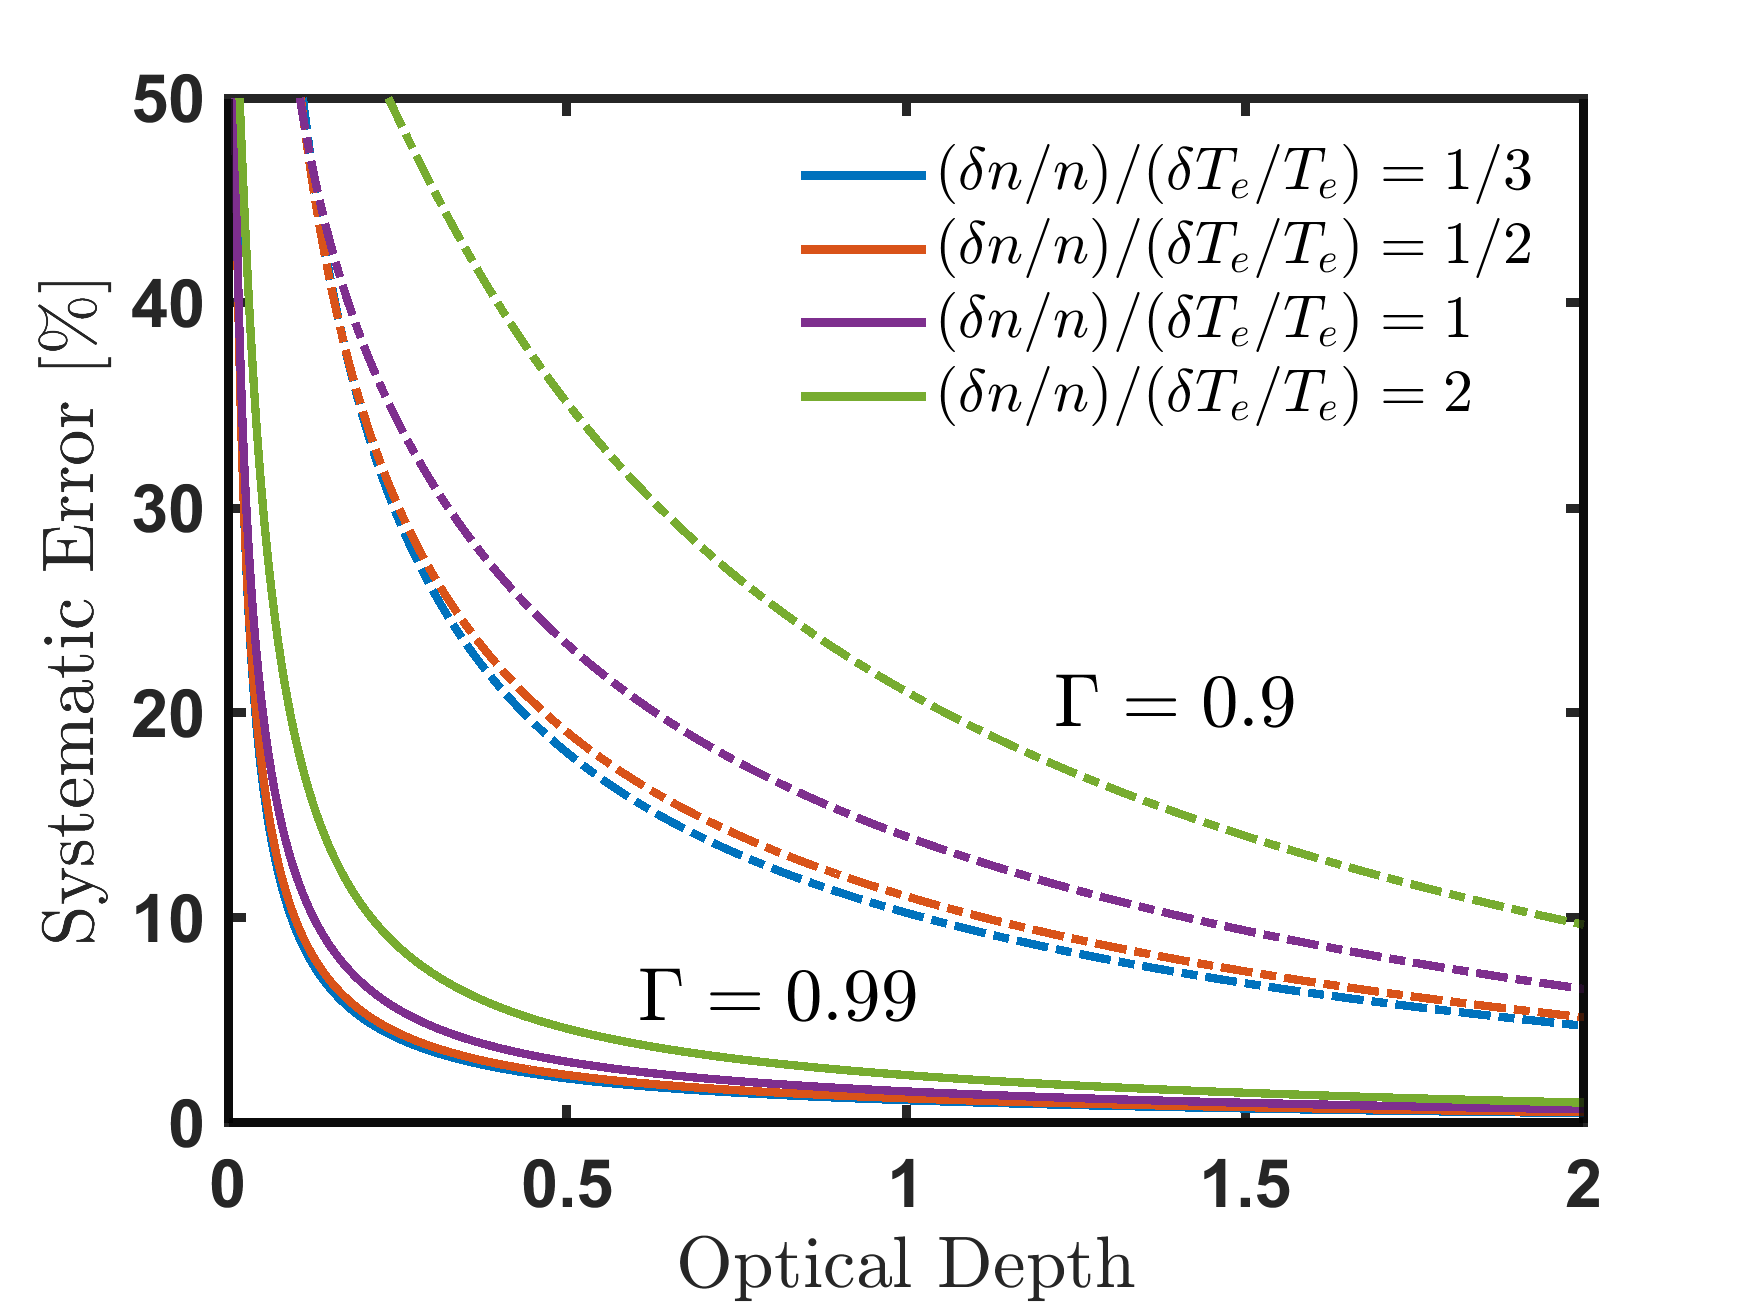
\includegraphics[width=.45\textwidth]{Figures/ratio_scan.png}}

\caption{Systematic error in interpreting radiation temperature fluctuations as electron temperature fluctuations as a function of optical depth, assuming in-phase density and electron temperature fluctuations. The error is shown for two values of effective vessel reflectivity $\Gamma$ and various ratios of $\delta n / n$ to $\delta T_e / T_e$. }
\label{fig:sys_error_ratio_scan}

\end{figure}  

Modeling is required to estimate the difference between $\delta T_r/T_r$ as $\delta T_e/T_e$. A systematic error in interpreting $\delta T_r/T_r$ as $\delta T_e/T_e$ can be derived by rearranging Eq.\ \eqref{eq:single_trad}. This error accounts for both the discrepancy between $T_r$ and $T_e$ and the discrepancy between $\delta T_r$ and $\delta T_e$ due to low optical depth and may be written as
\begin{align}
	E(\tau,\Gamma,\delta T_e/T_e, \delta n/n) = \left(1 + \frac{\delta n / n}{\delta T_e / T_e} \right) A_2(\tau,\Gamma),  \label{eq:error_est}
\end{align}
where $\alpha_{nT}$ is the density-temperature cross-phase and as before, $\Gamma$ is an effective vessel reflectivity. Here, an in-phase relationship between $\delta T_e/T_e$ and $\delta n/n$ is assumed, such that the modification by $\delta n/n$ is maximal and the calculated error is conservative. Eq.\ \eqref{eq:error_est} represents the factor by which $\delta T_r/T_r$ exceeds $\delta T_e/T_e$, and is used to derive a range of possible $\delta T_e/T_e$ based on $\delta T_r/T_r$ measurements presented in Chapter 4. Nonlinear gyrokinetic phase analysis presented in Chapter 5 suggests that $\alpha_{nT}\approx0$ in the wavenumber range accessible to CECE, indicating that this worst-case (in the sense that $\delta T_e/T_e$ maximally deviates from $\delta T_r/T_r$) systematic error analysis is appropriate.

Of the parameters that determine the systematic error in Eq.\ \eqref{eq:error_est}, only the optical is well-known for a given discharge. The optical depth is determined via raytracing with the TRAVIS code. The remaining parameters are the effective vessel reflectivity and ratio of $\delta n/n$ to $\delta T_e/T_e$. As previously mentioned, the stainless steel vacuum vessel of HSX has a theoretical reflectivity of $\Gamma=0.99$, and the agreement between absolutely calibrated ECE profile measurements and Thomson scattering in a relatively high-density QHS HSX discharge empirically suggests a near-unity reflectivity. A reflectivity $\Gamma=0.9$ was used to estimate a similar systematic error for heat pulse propagation experiments on HSX \cite{weir-thesis} and was expected to be a pessimistic value. Therefore, both $\Gamma=0.9$ and $\Gamma=0.99$ are considered in modeling the systematic error.

The range of reasonable ratios of $\delta n/n$ to $\delta T_e/T_e$ to consider for estimating systematic error due to low optical depth is motivated in part by experimental measurements and gyrokinetic modeling. Interferometer measurements of line-integrated $\delta n /n$, which were localized using a differential technique \cite{deng2015core}, found values up to 0.5\% in the wavenumber range $k_y < 2$ \,cm\textsuperscript{-1} and frequency range 20-120\,kHz. This wavenumber range is nearly equivalent to that of CECE. Previous reflectometer measurements of $\delta n/n$ at the mid-radius in HSX suggest amplitudes up to approximately 1\% in the wavenumber range $0.2 < k_y \rho_s < 1.0$. The radiation temperature fluctuations presented in Chapter 4 are measured in the range $2-6\%$. Assuming that up to 1\% of the measured $\delta T_r/T_r$ is comprised of $\delta n/n$ leads to a possible range of $\delta T_e/T_e$ between $1-5\%$, and a range of $(\delta n/n)/(\delta T_e/T_e)$ of $1/5-1$.  Gyrokinetic modeling presented in Chapter 5 suggests that at finite electron temperature gradient, $(\delta n/n)/(\delta T_e/T_e) \geq 1$ in the wavenumber range accessible to CECE. Considering both experimental results and gyrokinetic modeling, the range $(\delta n/n)/(\delta T_e/T_e)$ of $1/3-2$ was chosen: a lower bound of $1/3$ rather than $1/5$ was chosen because the error was found to change very little below this value, and an upper bound of double the expected ratio (which leads to higher error) was chosen to assess a nominal upper bound on the error. The systematic error as a function of optical depth for these ratios is shown in Fig.\ \ref{fig:sys_error_ratio_scan}. Relevant optical depth values in HSX are $0.1 < \tau < 1.5$ for the discharges considered in this work.

The systematic error in interpreting $\delta T_r/T_r$ depends critically on the effective wall reflectivity. Fig.\ \ref{fig:sys_error_ratio_scan} shows that over the range of considered density to temperature fluctuation ratios, the systematic over-prediction of $\delta T_e/T_e$ is negligibly different at the theoretical upper bound on the reflectivity $\Gamma=0.99$. This is expected, as a near-unity reflectivity leads to a low value of the parameter $A_2$ appearing in Eq.\ \eqref{sec:sys_error}, except at very marginal optical depths. Below an optical depth $\tau\equiv\tau_{crit}=0.2$, $A_2$ begins to increase rapidly, corresponding with the sharp growth in the systematic error at low optical depth in Fig.\ \ref{fig:sys_error_ratio_scan}. Below this critical optical depth, it is not reasonable to interpret $\delta T_r/T_r$ as $\delta T_e/T_e$, and therefore measurements of $\delta T_r/T_r$ reported in Chapter 4 are shown above this value only.

At an assumed reflectivity $\Gamma=0.9$, the increase in systematic error with increasing ratio of density to electron temperature fluctuations is higher at equal optical depth than with a reflectivity $\Gamma=0.99$. For $(\delta n/n)/(\delta T_e/T_e) < 1$, the systematic error at $\tau=\tau_{crit}$ is approximately 50\%. The optical depth for which the systematic error is below 50\%, considering a pessimistic upper bound of $(\delta n/n)/(\delta T_e/T_e)=2$, is approximately $\tau=0.3$, just above the defined critical optical depth. For optical depths above 0.5, the systematic error is modeled to be less than 30\%, independent of fluctuation ratio, at $\Gamma=0.9$. Despite the large modeled systematic uncertainties in Fig.\ \ref{fig:sys_error_ratio_scan}, the experimental results in Chapter 4 will demonstrate that there is little ambiguity in the fact that there are measurable core electron temperature fluctuations in HSX, in part because the measured $\delta T_r/T_r$ amplitudes are high.



%%%%%%%%%%%%%%%%%%%%%%%%%%%%%%%%%%%%%%%%%%%%%%%%%%%%%%%%%%%%%%%%%%%%%%%%%%%%%%%%%%%%%%%%%%%%%%%%%%%%%%%%%%%%%%%%%%%%%%
\section{\label{sec:exp_cece} Radiation Temperature Fluctuation Measurements} 
%%%%%%%%%%%%%%%%%%%%%%%%%%%%%%%%%%%%%%%%%%%%%%%%%%%%%%%%%%%%%%%%%%%%%%%%%%%%%%%%%%%%%%%%%%%%%%%%%%%%%%%%%%%%%%%%%%%%%%

\section{Radiation and Electron Temperature Fluctuations in QHS Plasmas} 

% \subsection{Base Case: $\delta T_r/T_r$  in High Density QHS Plasma}
CECE measurements in optically semi-transparent HSX plasma can be interpreted as local electron temperature fluctuations when plasma optical depth is sufficiently high. The modeling presented in Section \ref{sec:sys_error} shows that the systematic error in interpreting $\delta T_r/T_r$ as $\delta T_e/T_e$ is acceptable above an optical depth $\tau_\mathrm{crit}=0.2$ assuming a near-unity effective vessel reflectivity. A reflectivity of $\Gamma=0.9$, expected to be an underestimate in HSX, leads to a 50\% systematic over-prediction of $\delta T_e/T_e$ at $\tau=\tau_{crit}$, and this error drops below 30\% for optical depths above 0.5. The discharge conditions that maximize optical depth are those that maximize electron pressure. Several high optical depth discharge conditions are analyzed in this section. Discharge dates and shot numbers can be found in Appendix \ref{app:C}.


\subsection{Base Case: High-density Hydrogen-fueled Discharges}

\begin{figure}[!htbp]
\begin{subfigure}[]{0.45\textwidth}
  \subfloat[]{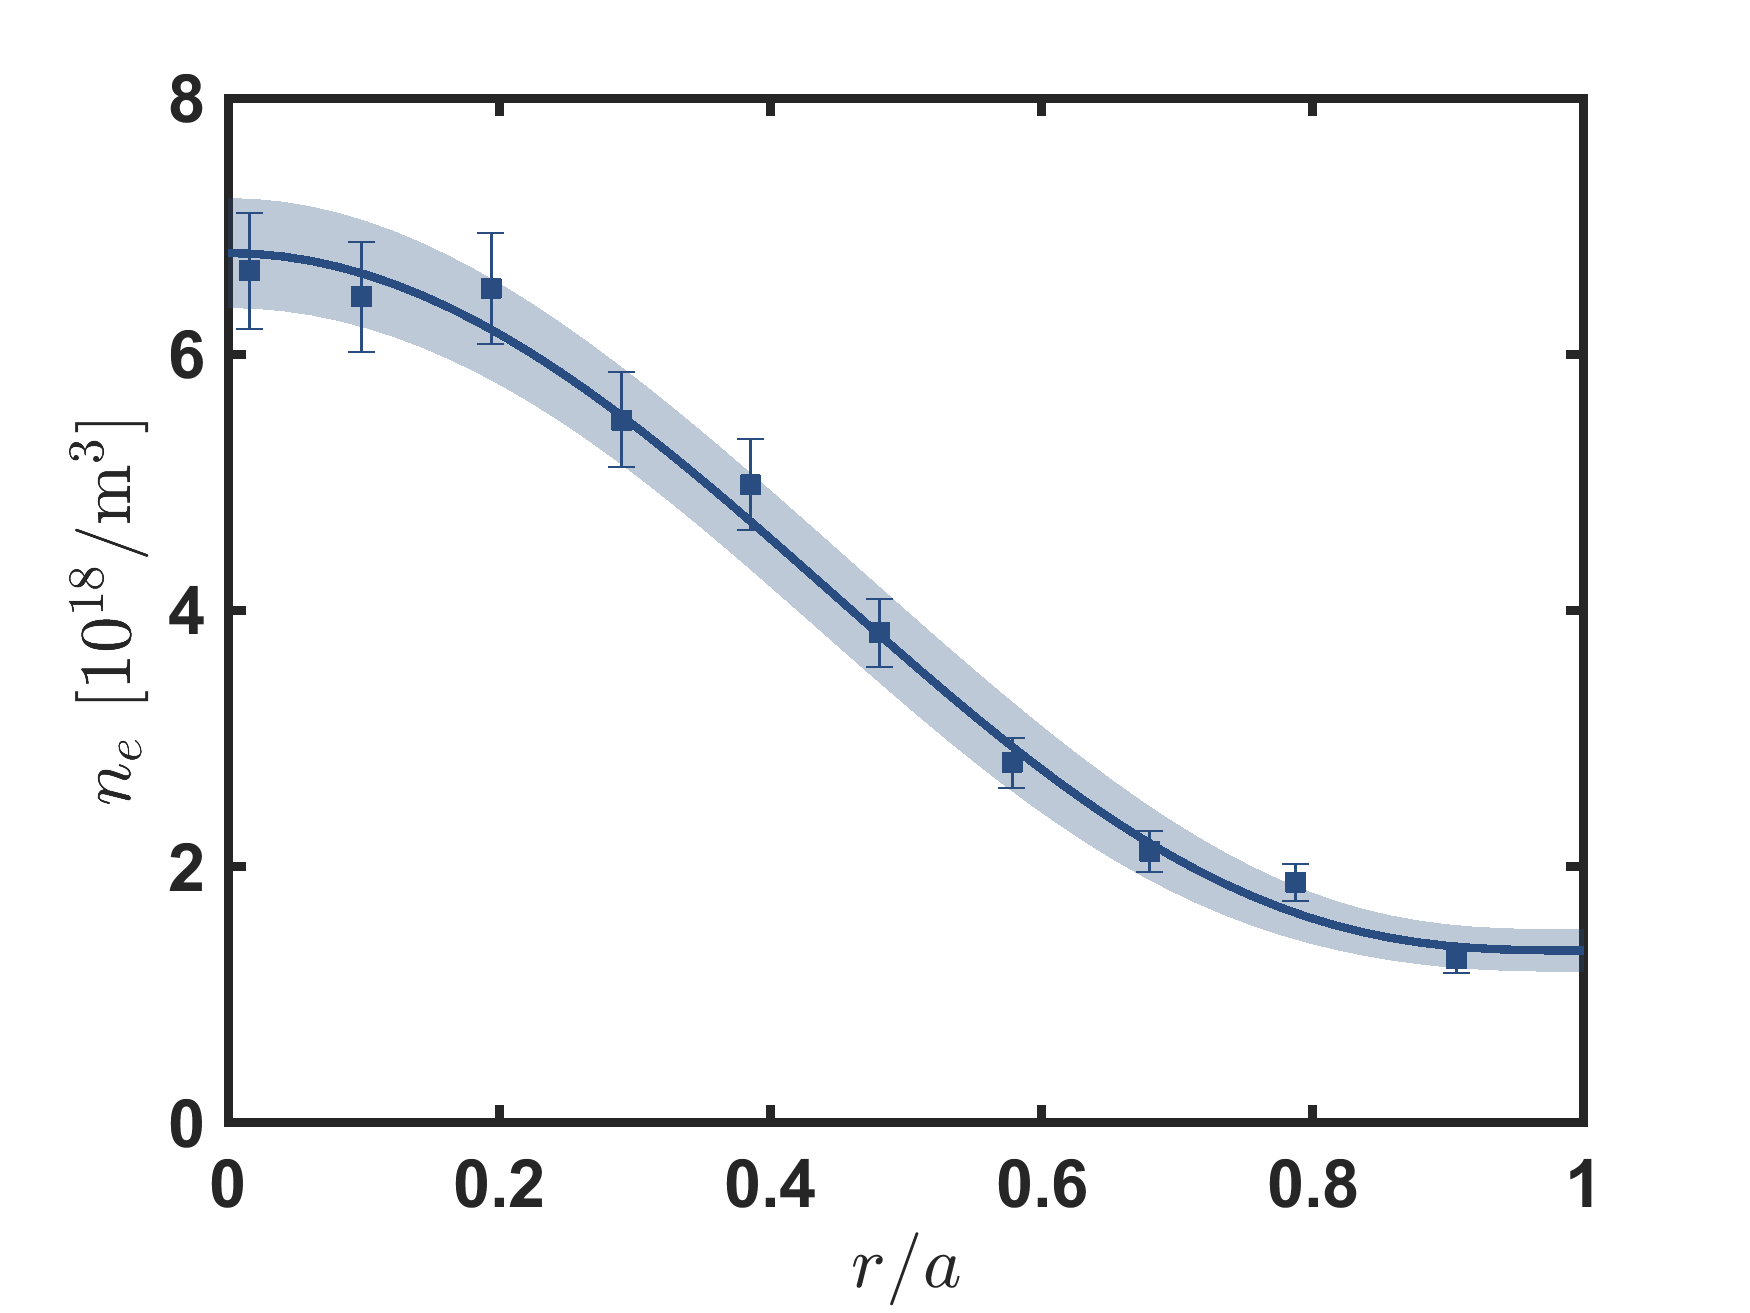
\includegraphics[width=\textwidth]{Figures/base_case_ne_a.png}}
\end{subfigure}
\hfill
\begin{subfigure}[]{0.45\textwidth}
  \subfloat[]{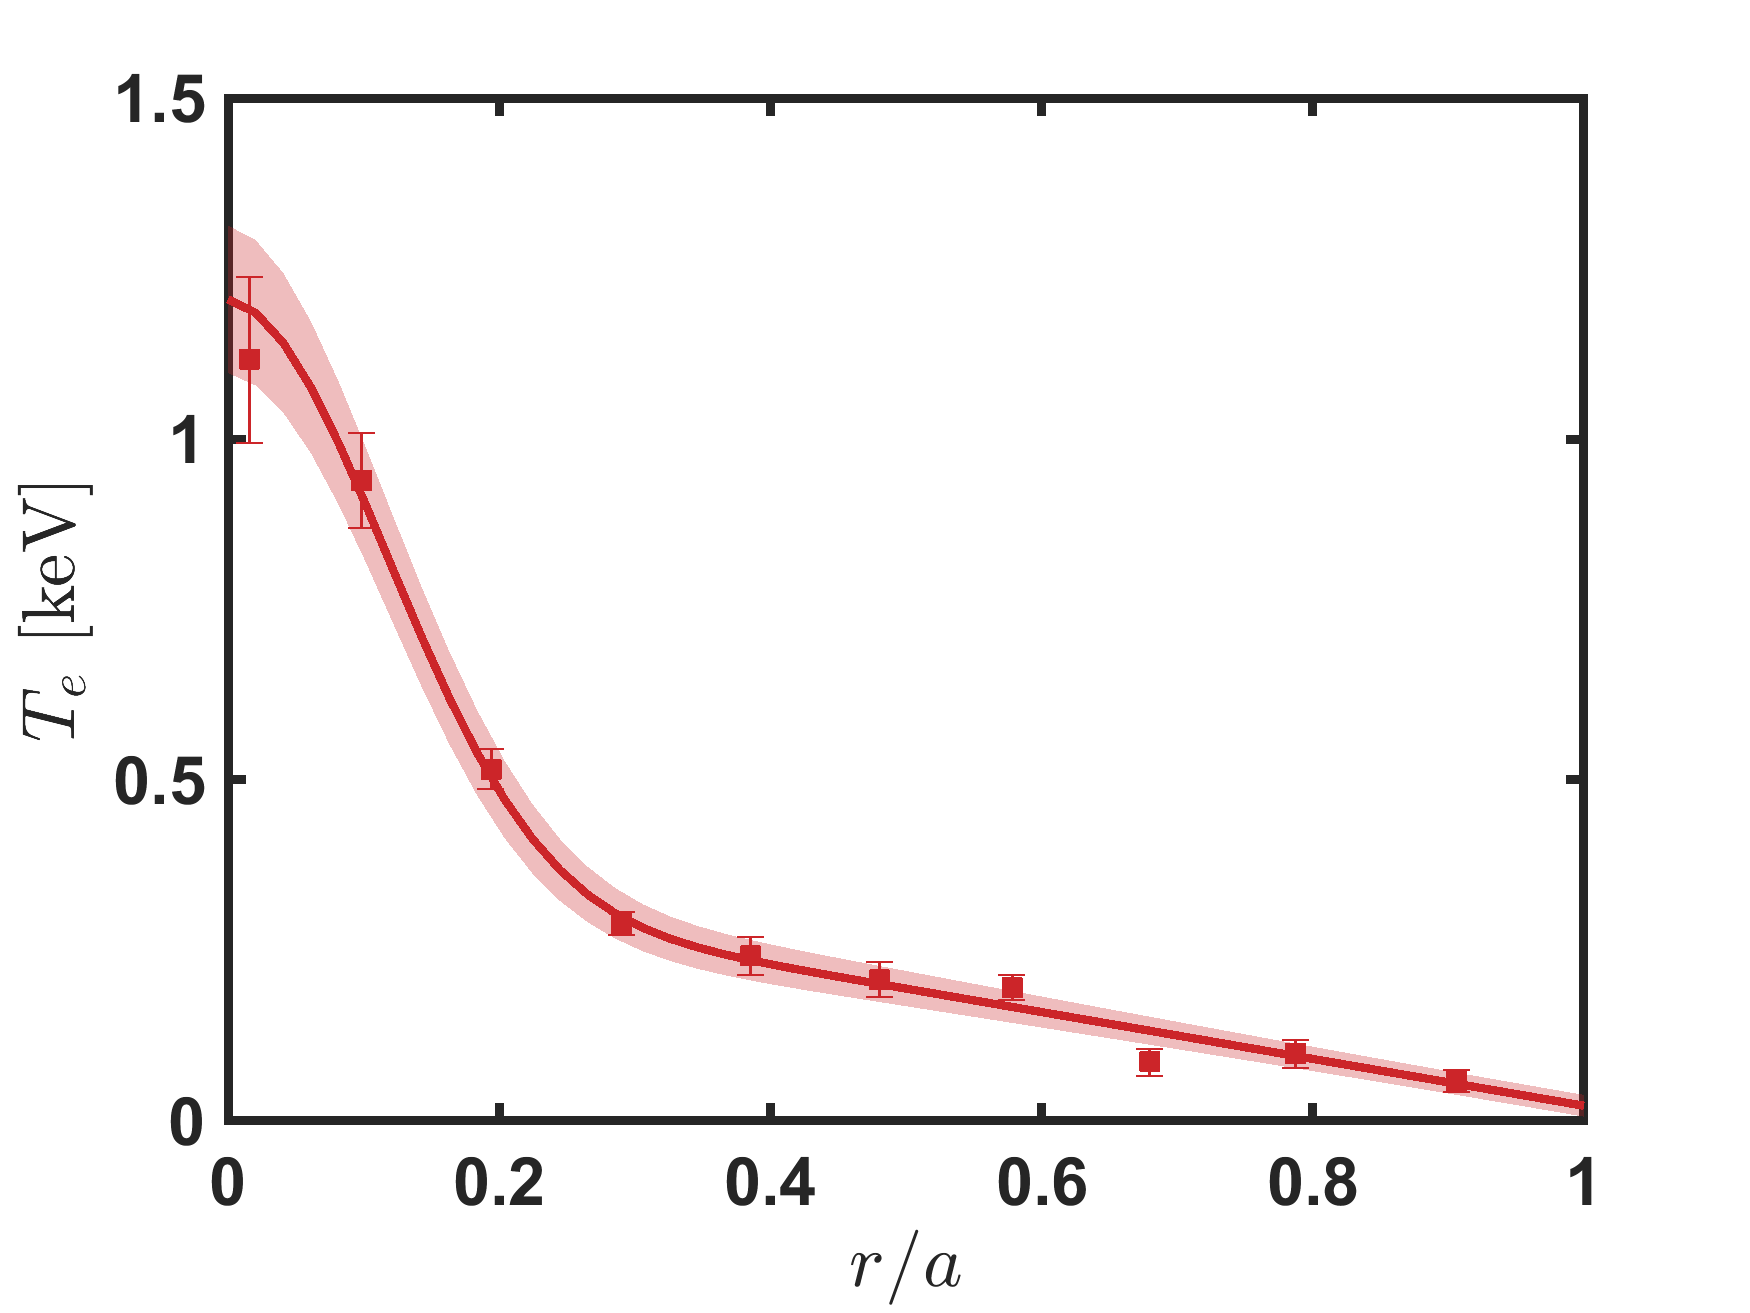
\includegraphics[width=\textwidth]{Figures/base_case_Te_b.png}}
\end{subfigure}

\caption{MCMC fits (solid lines) to Thomson scattering data (markers) of (a) plasma density and (b) electron temperature for the base case (see text).}
\label{fig:nT_base_case}
\end{figure}

Hydrogen fueling is used for the majority of HSX experiments performed to date. Electron profiles for a high-density hydrogen-fueled QHS discharge with 50 kW launched ECRH power are shown in Fig.\ \ref{fig:nT_base_case}, calculated using an ensemble of five repeatable discharges to improve the photon statistics of the Thomson scattering diagnostic \cite{canik2007experimental,lore2010measurement}. The Thomson scattering raw data is fit using a Markov Chain Monte Carlo (MCMC) routine \cite{foreman2013emcee}. The time trace of plasma line-averaged density, stored energy, and a core high-field side ECE channel is shown in Fig.\ \ref{fig:base_status_plot}. The on-axis $n_e$ for these discharge conditions is near the upper limit observed in HSX. The absorbed power in these discharges is $P_{abs}=12.4 \pm 1.4$\,kW, and the energy confinement time is $\tau_E=4.0 \pm 0.5$\,ms, based on diamagnetic loop measurements. The profiles shown in Fig.\ \ref{fig:nT_base_case} will be used as a point of comparison with several additional discharge conditions in this chapter and will be referred to as the \textit{base case}.


\begin{figure}[!htbp]
\centering
\begin{subfigure}[]{0.45\textwidth}
  \centering
  \subfloat[]{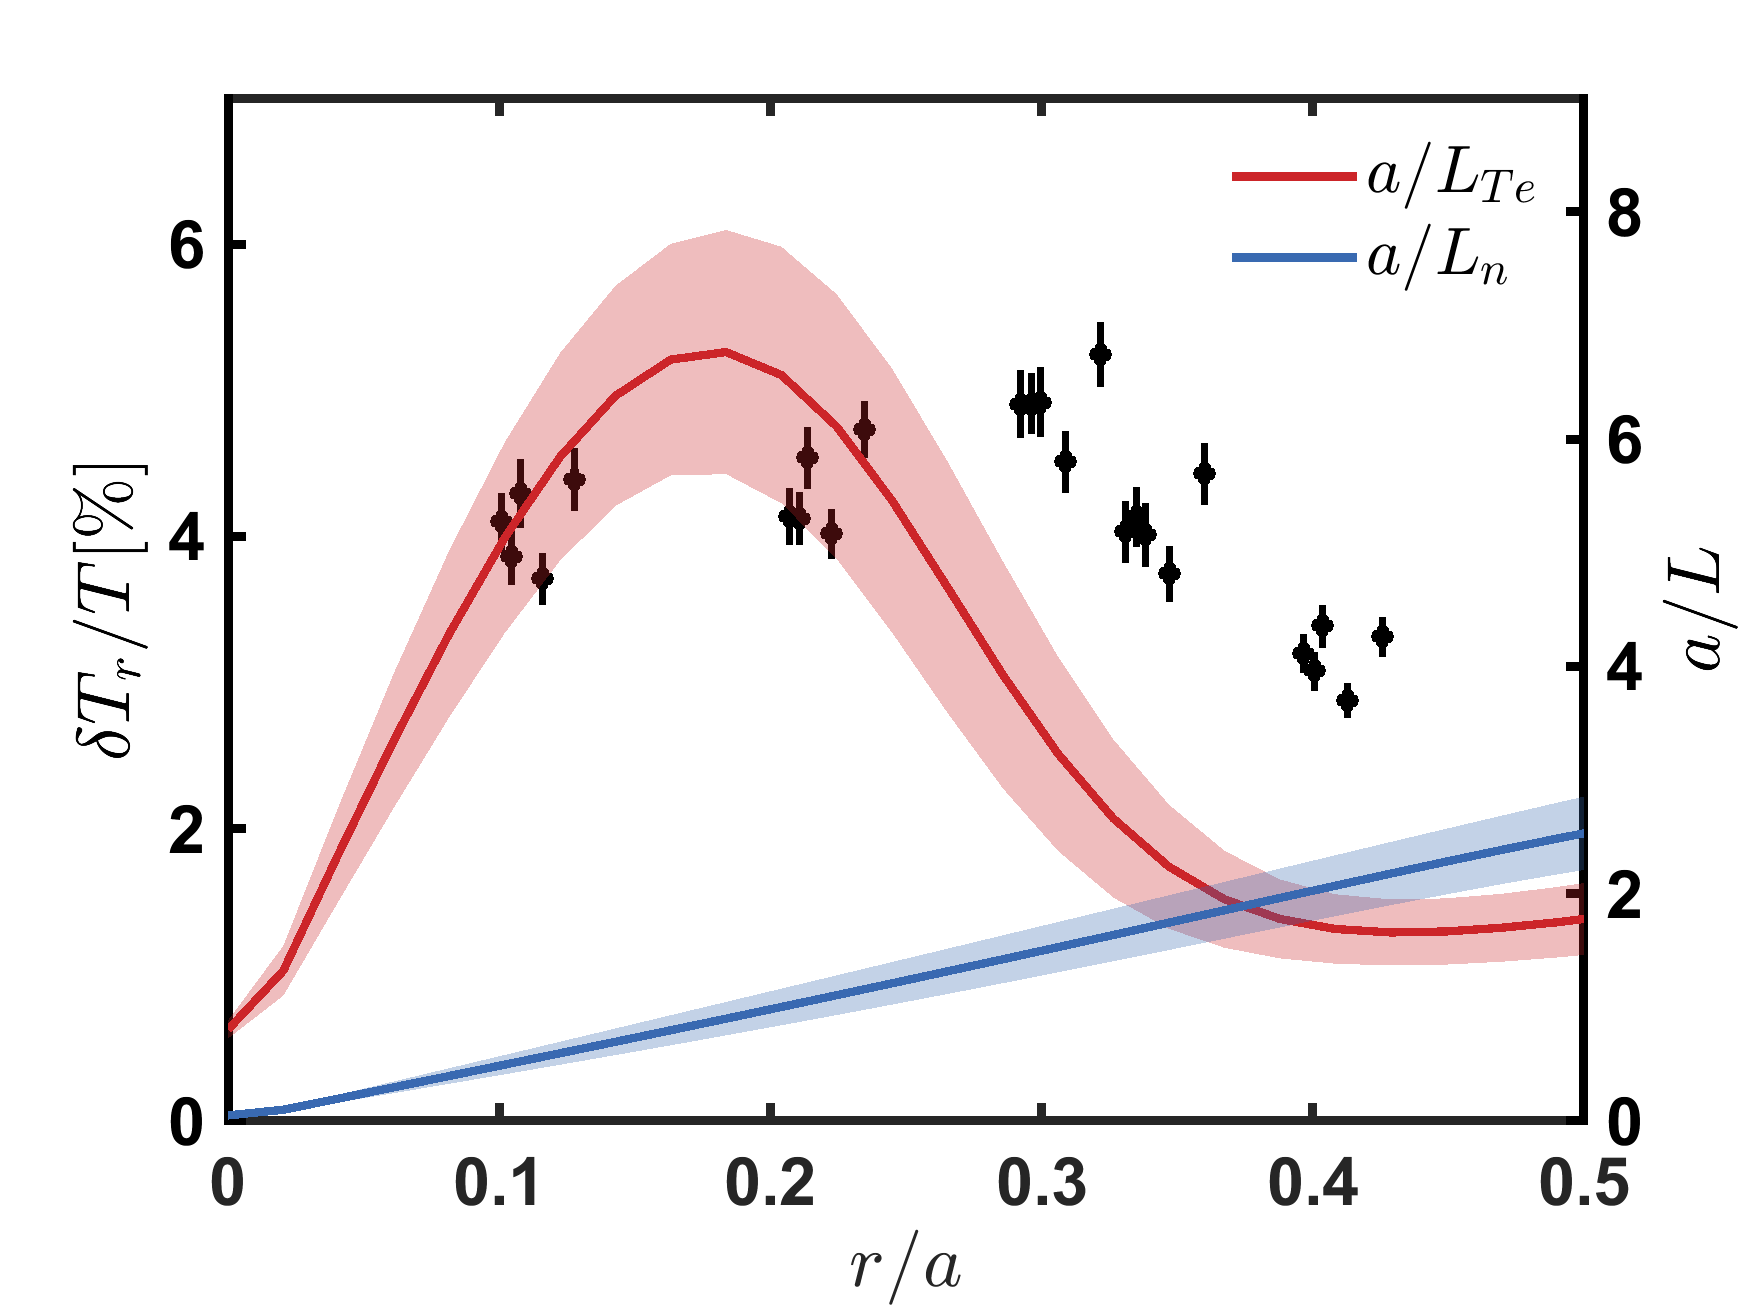
\includegraphics[width=\textwidth]{Figures/base_case_overlay_final.png}}
\end{subfigure}
\hfill
\begin{subfigure}[]{0.45\textwidth}
  \centering
  \subfloat[]{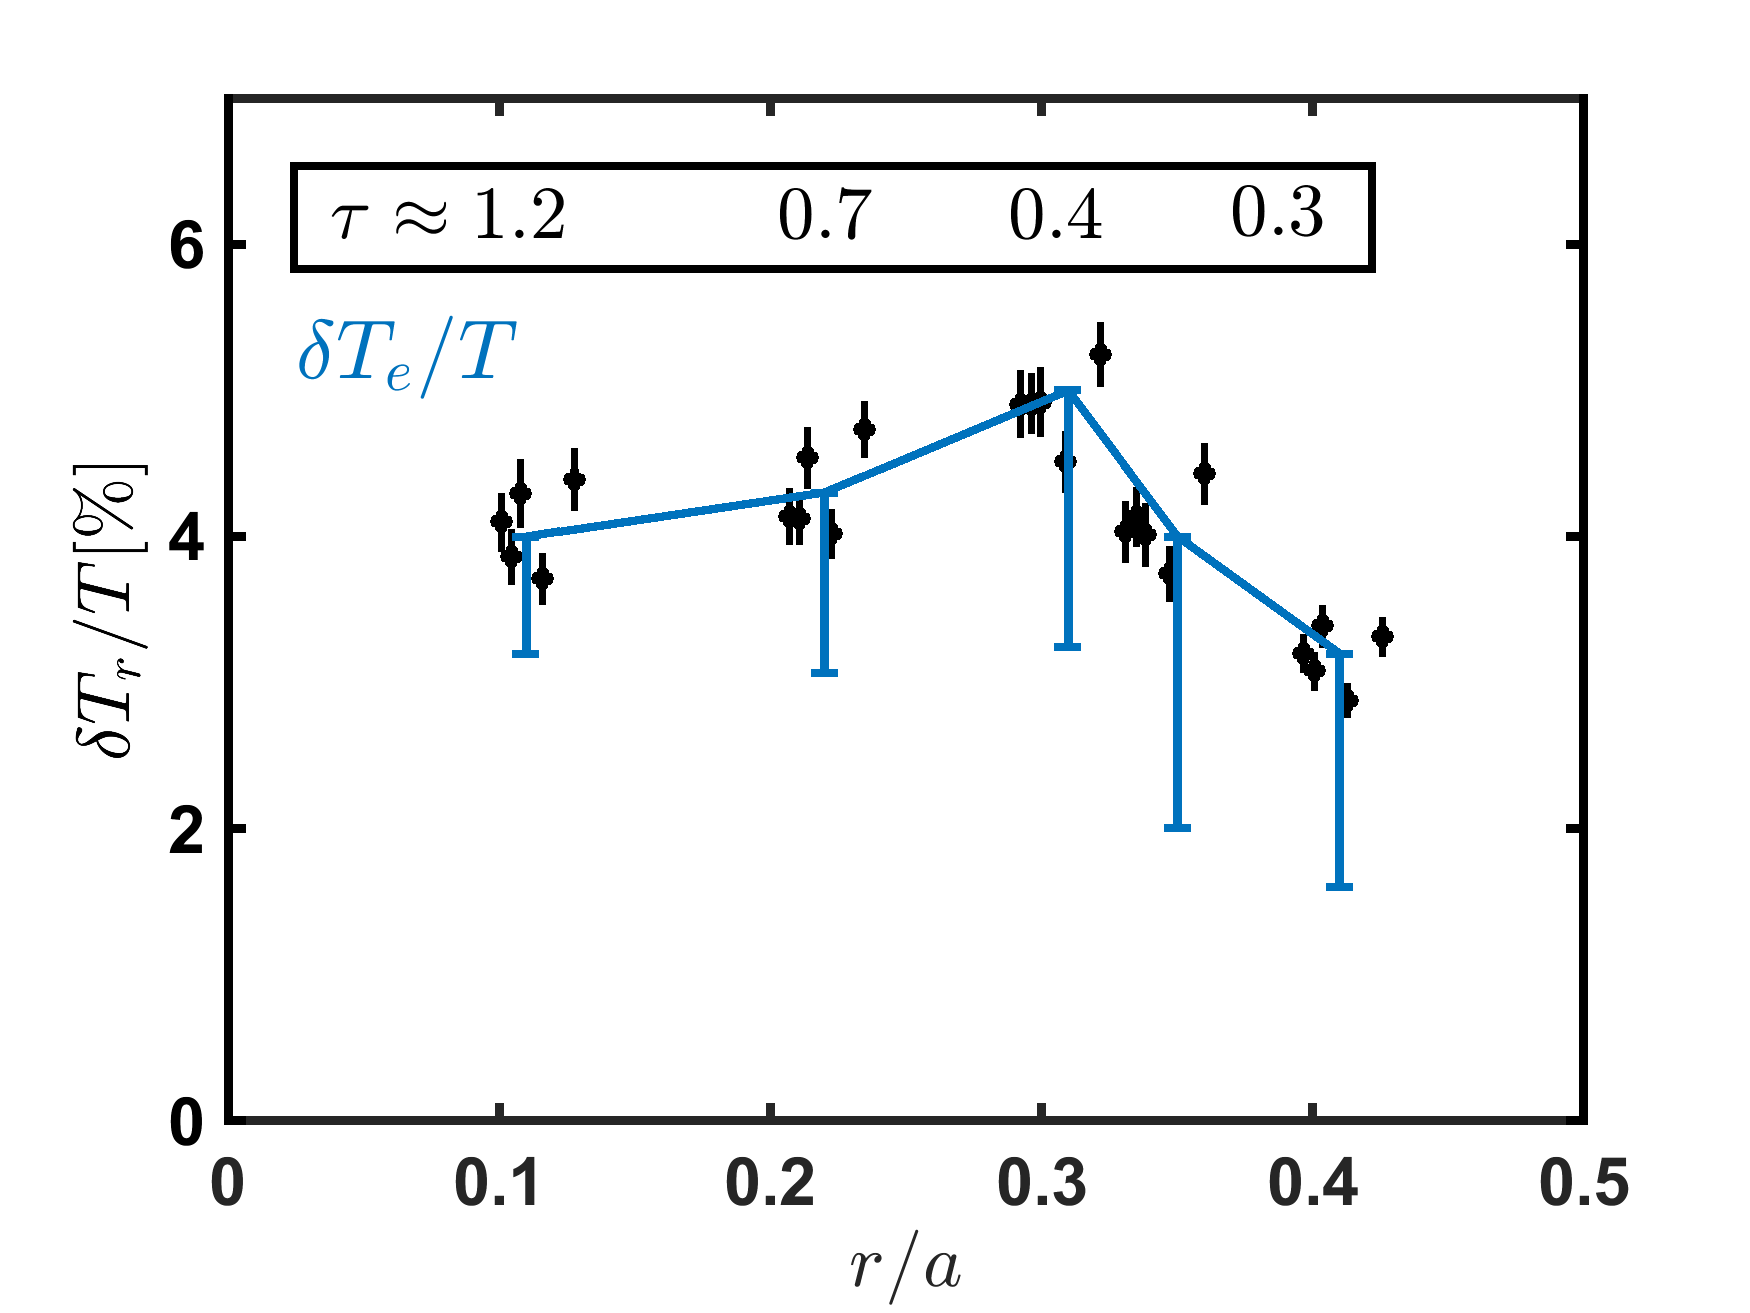
\includegraphics[width=\textwidth]{Figures/base_case_tau_error2.png}}
  %\label{fig:bimax_setup}
\end{subfigure}

\caption{(a) $\delta T_r /T_r$ for five repeatable discharges used to generate a Thomson scattering profile, with normalized inverse gradient scale lengths of density and electron temperature overlaid, for the base case. Slight differences in main coil current produce different shot-to-shot channel localization. (b) The modeled range of $\delta T_e/T_e$  based on the indicated plasma optical depth and assuming a vessel reflectivity of $\Gamma=0.9$ using the systematic error estimate described in Section \ref{sec:sys_error} (see Eq.\ \eqref{eq:error_est}).}
\label{fig:base_case_summary}
\end{figure}


The radial profile of  $\delta T_r/T_r$  derived using the estimator M3 on the high-field side of the HSX magnetic axis is shown in Fig.\ \ref{fig:base_case_summary}(a). The fluctuations are indicated as black markers and are shown for each shot in the base case ensemble used to generate Thomson scattering profiles. Overlaid are the normalized inverse gradient scale lengths of density, $a/L_n$, and electron temperature, $a/L_{Te}$, derived from the profiles in Fig.\ \ref{fig:nT_base_case}. The fluctuation amplitude in the near-axis channel, $r/a\approx 0.1$, is approximately 4\%. The amplitude slightly increases with minor radius, peaking near $r/a=0.3$ at approximately 5\%. Within $0.3 < r/a < 0.4$, the amplitude decreases. The sample volume for the innermost ECE channels $r/a \approx 0.2$ is larger than the emitting volume, and in this sense, the measurements are line-integrated within $0 < r/a < 0.2$. In contrast, the measurements beyond $r/a > 0.2$ are radially localized. Note that several figures similar to Fig.\ \ref{fig:base_case_summary}(a) will be shown in this section. The y-axis ranges for $\delta T_r/T_r$ and $a/L$ are consistent between these plots and chosen to bracket the maximum reported values.

The scaling of $\delta T_r/T_r$ with $a/L_{Te}$ and $a/L_n$ is important for identifying different plasma turbulence regimes and assessing dominant instability mechanisms. For the base case, $a/L_n$ increases from approximately 0.7 to 1.5 over the radial range $0.1 \lesssim r/a \lesssim 0.3$, where $\delta T_r/T_r$  increases from approximately 4\% to 5\%. $a/L_{Te}$ varies non-monotonically in the same region in the range 4-7. Beyond $r/a\approx 0.3$, $a/L_{Te}$ drops from approximately $a/L_{Te}=7$ to $a/L_{Te}=2$ and $\delta T_r/T_r$ decreases from approximately 5\% to 3\%. Determining possible scaling of the fluctuation amplitude with driving gradients is difficult with a radial profile, as $a/L_n$ and $a/L_{Te}$ vary simultaneously. Within $r/a\approx0.3$, the increase in $\delta T_r/T_r$  may suggest that $\delta T_r/T_r$ increase with increasing $a/L_n$, but beyond $r/a\approx0.3$, $\delta T_r/T_r$ decrease while $a/L_n$ is still increasing. This decrease in fluctuation amplitude appears to track with decreasing $a/L_{Te}$, but the fluctuation amplitude does not peak at the maximum of $a/L_{Te}$.


In optically semi-transparent plasmas, density fluctuations can lead to a discrepancy between $\delta T_r/T_r$ and $\delta T_e/T_e$. Fig.\ \ref{fig:base_case_summary}(b) shows the same $\delta T_r/T_r$ amplitudes as in Fig.\ \ref{fig:base_case_summary}(a) and a modeled range of $\delta T_e/T_e$. This range is calculated using the measured $\delta T_r/T_r$ and the indicated plasma optical depth, $\tau$, using Eq.\ \eqref{sec:sys_error}. The effective vessel reflectivity is assumed to be $\Gamma=0.9$. Specifically, the indicated $\delta T_e/T_e$ ranges are computed using the average $\delta T_r/T_r$ over all five discharges, and similarly, the minor radial location is taken as the average location. Fig.\ \ref{fig:base_case_summary}(b) shows that there may be a large discrepancy between the measured $\delta T_r/T_r$ and corresponding $\delta T_e/T_e$. However, $\delta T_r/T_r$ is not expected to reflect only density fluctuations. Within $r/a=0.3$, the minimum $\delta T_e/T_e$  amplitude is expected to be approximately 3\%, and beyond $r/a=0.3$ may be as low as approximately 1.5\%. Whereas $\delta T_r/T_r$ decrease beyond $r/a=0.3$, this is less clear for $\delta T_e/T_e$  due to the high systematic uncertainty. Within $r/a\approx0.4$, a constant $\delta T_e/T_e$ amplitude cannot be ruled out.

An important aspect of the systematic error analysis used to generate the $\delta T_e/T_e$ ranges in Fig.\ \ref{fig:base_case_summary}(b) is that it cannot account for the possible change in $\delta n/n$ with minor radius (in the absence of $\delta n/n$ measurements). Previous measurements suggest that $\delta n/n$ increase with increasing $a/L_n$ (see Section \ref{sec:hsx_turbo_review}), which increases with radius in these discharges and in all discharges shown in this section. Therefore, in-phase $\delta n/n$ contributions to $\delta T_r/T_r$ are expected to increase with minor radius. As a result, the proportion of $\delta T_e/T_e$ contributing to $\delta T_r/T_r$  is expected to decrease with minor radius, and $\delta T_e/T_e$  would be expected to fall lower within the indicated $\delta T_e/T_e$ range at higher minor radius. Hence, a constant $\delta T_e/T_e$ beyond $r/a\approx0.3$ is not likely based on previous measurements.


\subsection{High On-axis $T_e$ Methane-fueled Discharges} \label{sec:methane_flucs}

%\subsection{High $T_e$ CH\textsubscript{4} Plasma}
Very high core electron temperatures have been observed in the QHS configuration, with peak recorded temperatures up to approximately 3\,keV. Many of the highest $T_e$ plasmas have been achieved with methane fueling. In plasma experiments with CECE, the highest on-axis $T_e$ and $a/L_{Te}$ were observed in high-power methane discharges. Profiles for an ensemble of repeatable discharges with these conditions are shown in Fig.\ \ref{fig:methane_fluc_summary}(a-b). For these plasmas, the line-averaged density is $n_e=3.5\times$10\textsuperscript{18}\,m\textsuperscript{-3}, and diamagnetic loop measurements indicate $P_{\mathrm{abs}}=22.1\pm1.8$\,kW and $\tau_E=3.2\pm0.2$\,ms.

\begin{figure*}[!htbp]
\centering
\begin{subfigure}[]{.45\textwidth}
  \centering
  \subfloat[]{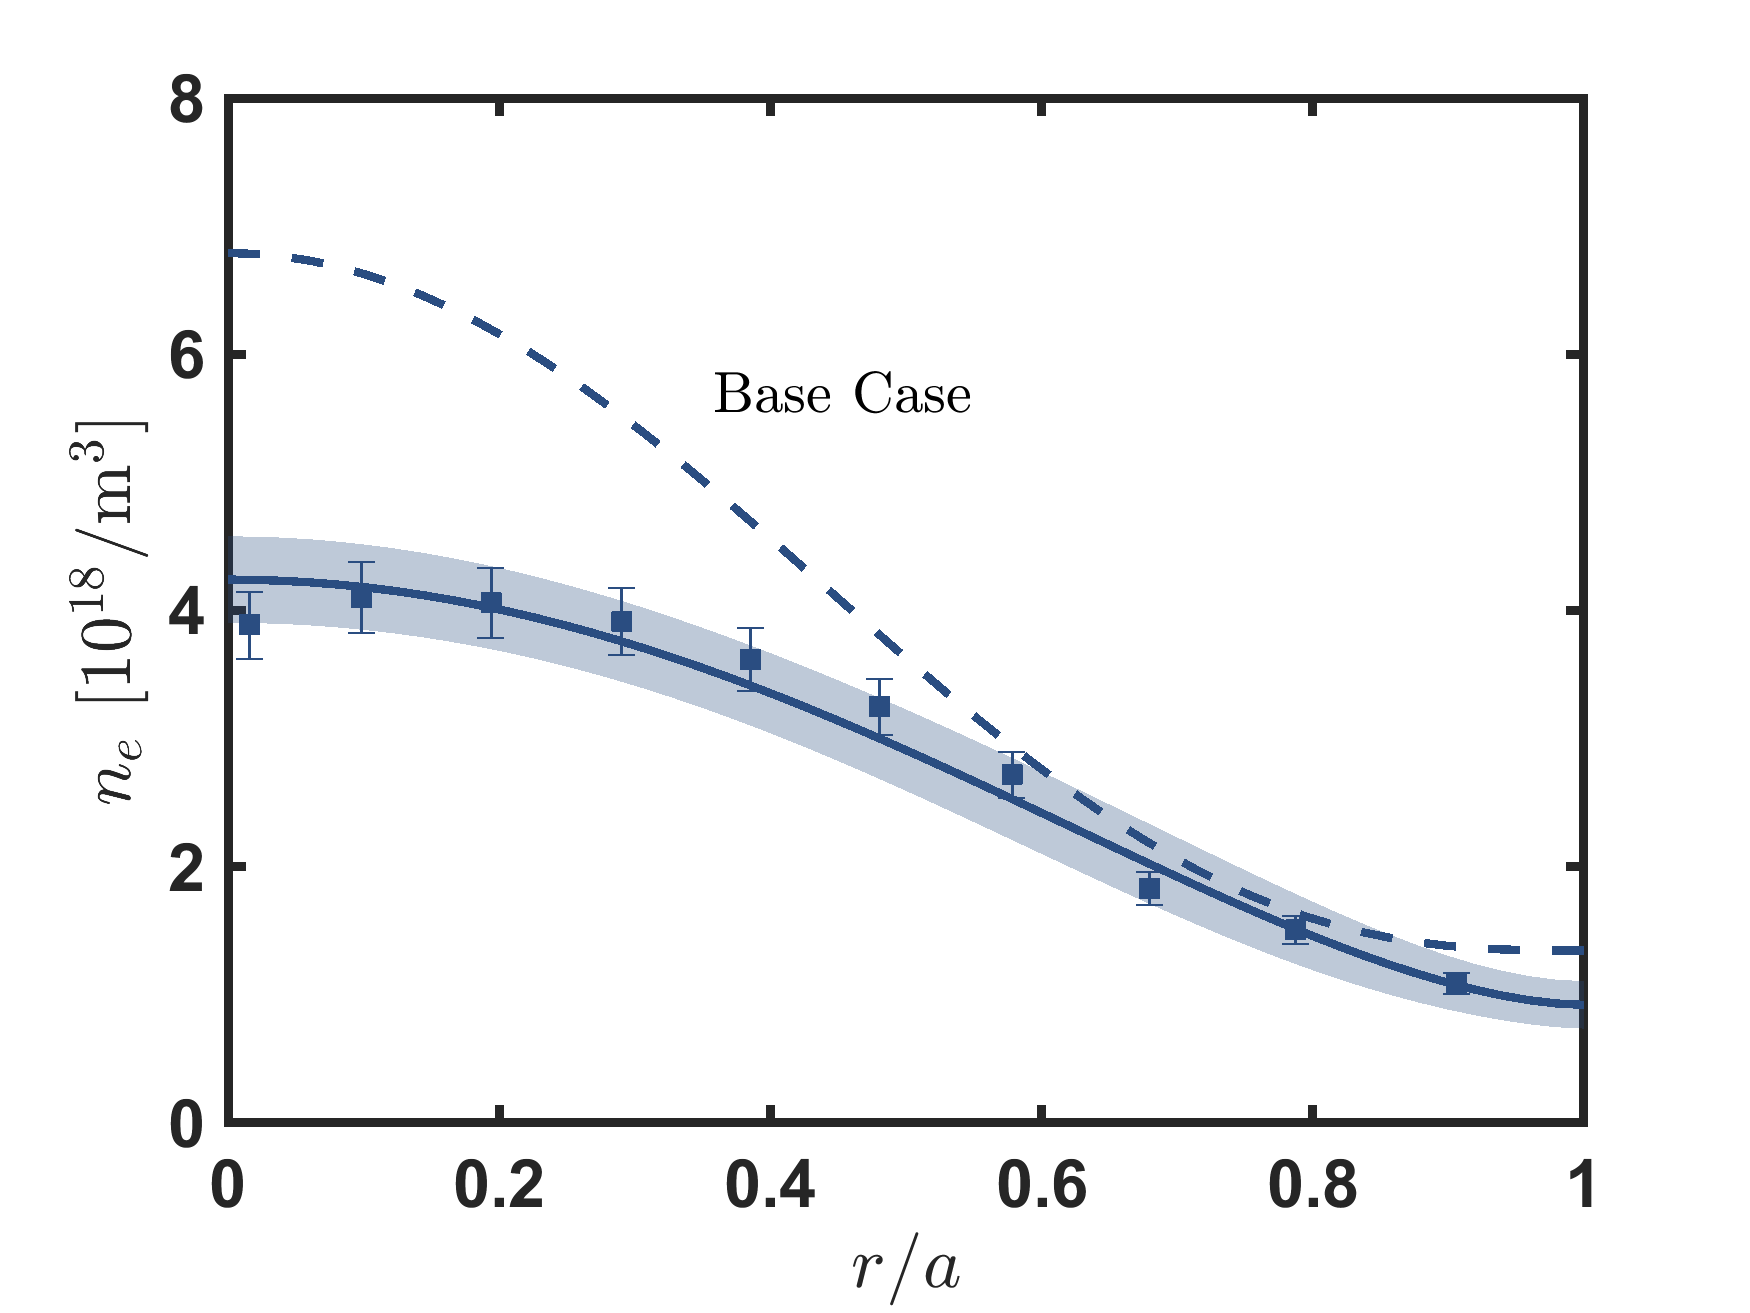
\includegraphics[width=\textwidth]{Figures/h2_ch4_ne_overlay_a.png}}
\end{subfigure}
\hfill
\begin{subfigure}[]{.45\textwidth}
  \centering
  \subfloat[]{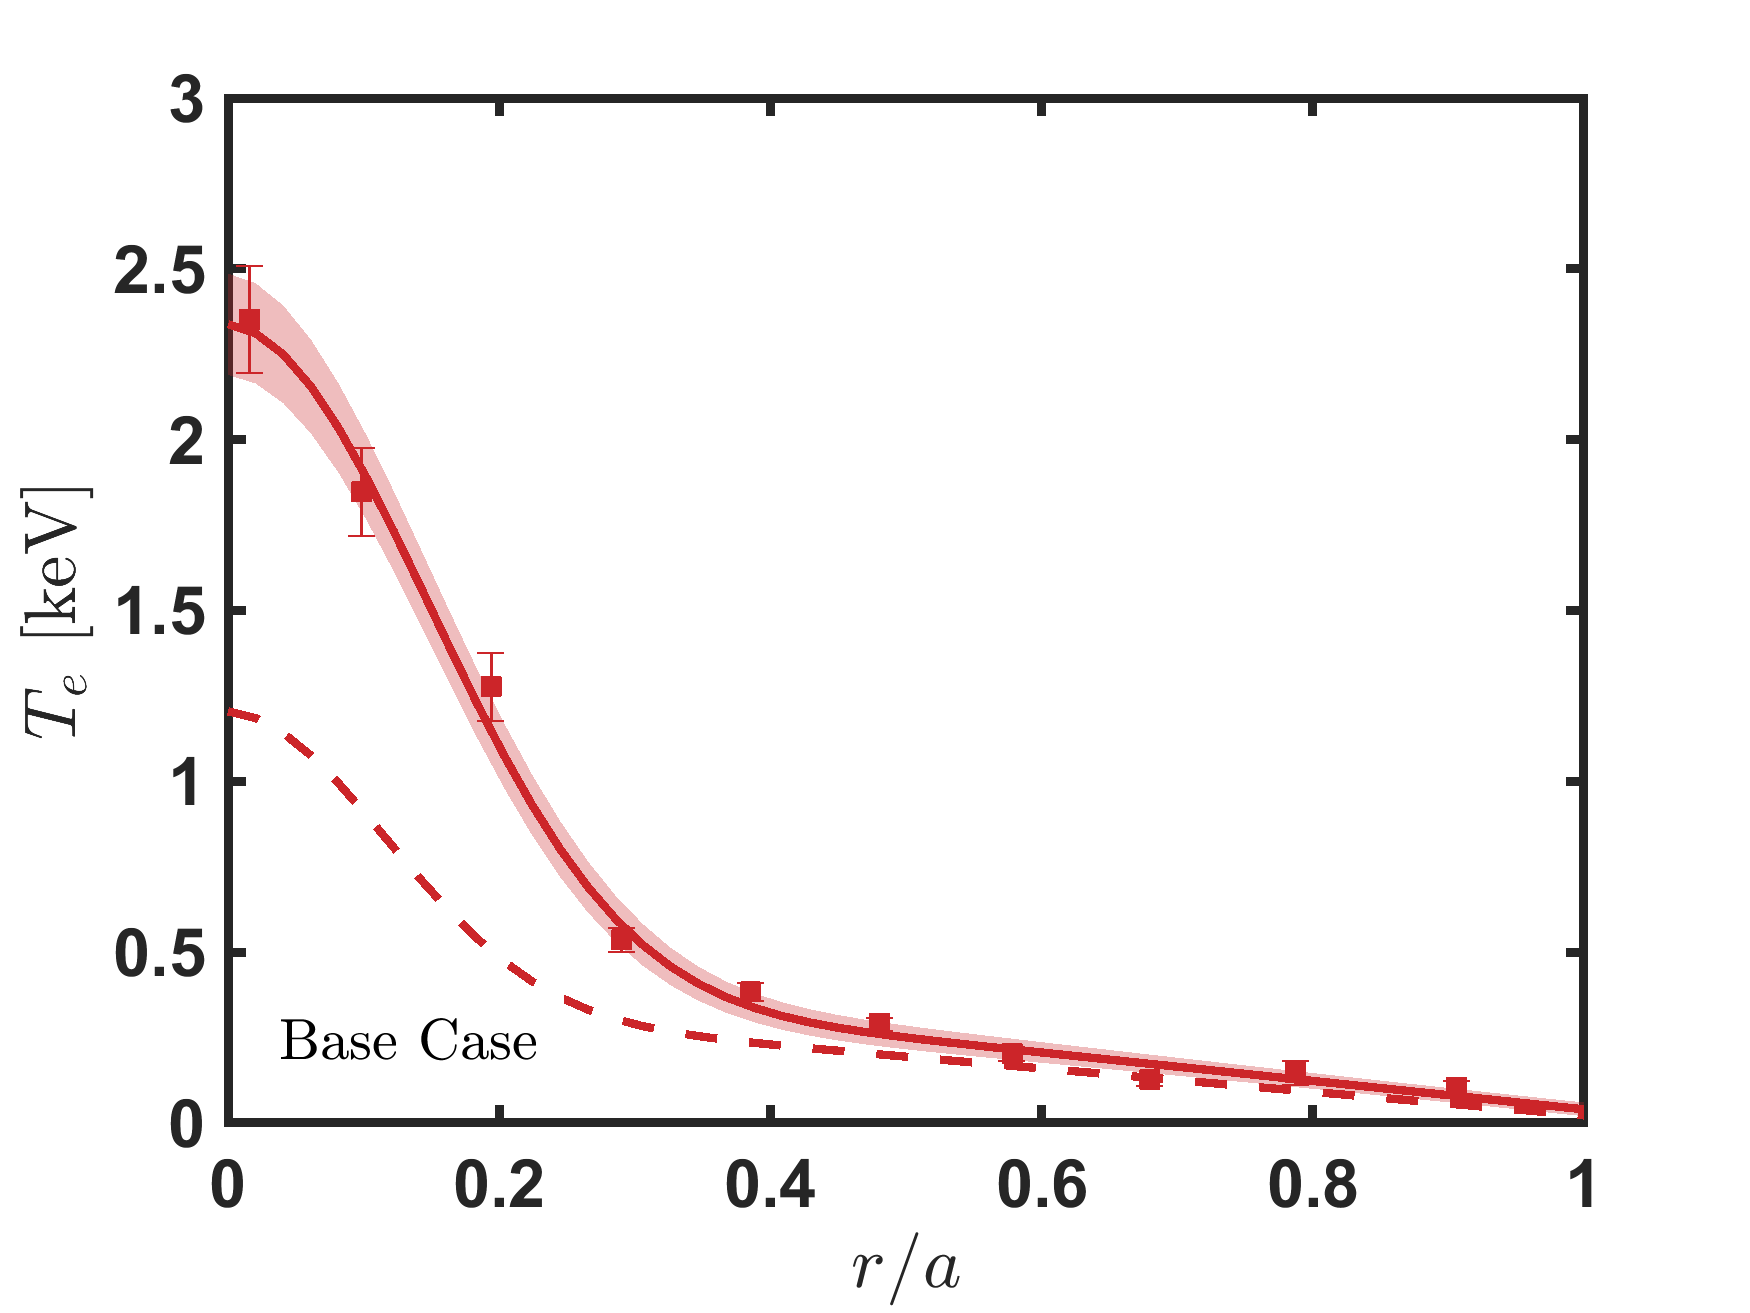
\includegraphics[width=\textwidth]{Figures/h2_ch4_Te_overlay_b.png}}

\end{subfigure}
\begin{subfigure}[]{.45\textwidth}
  \centering
  \subfloat[]{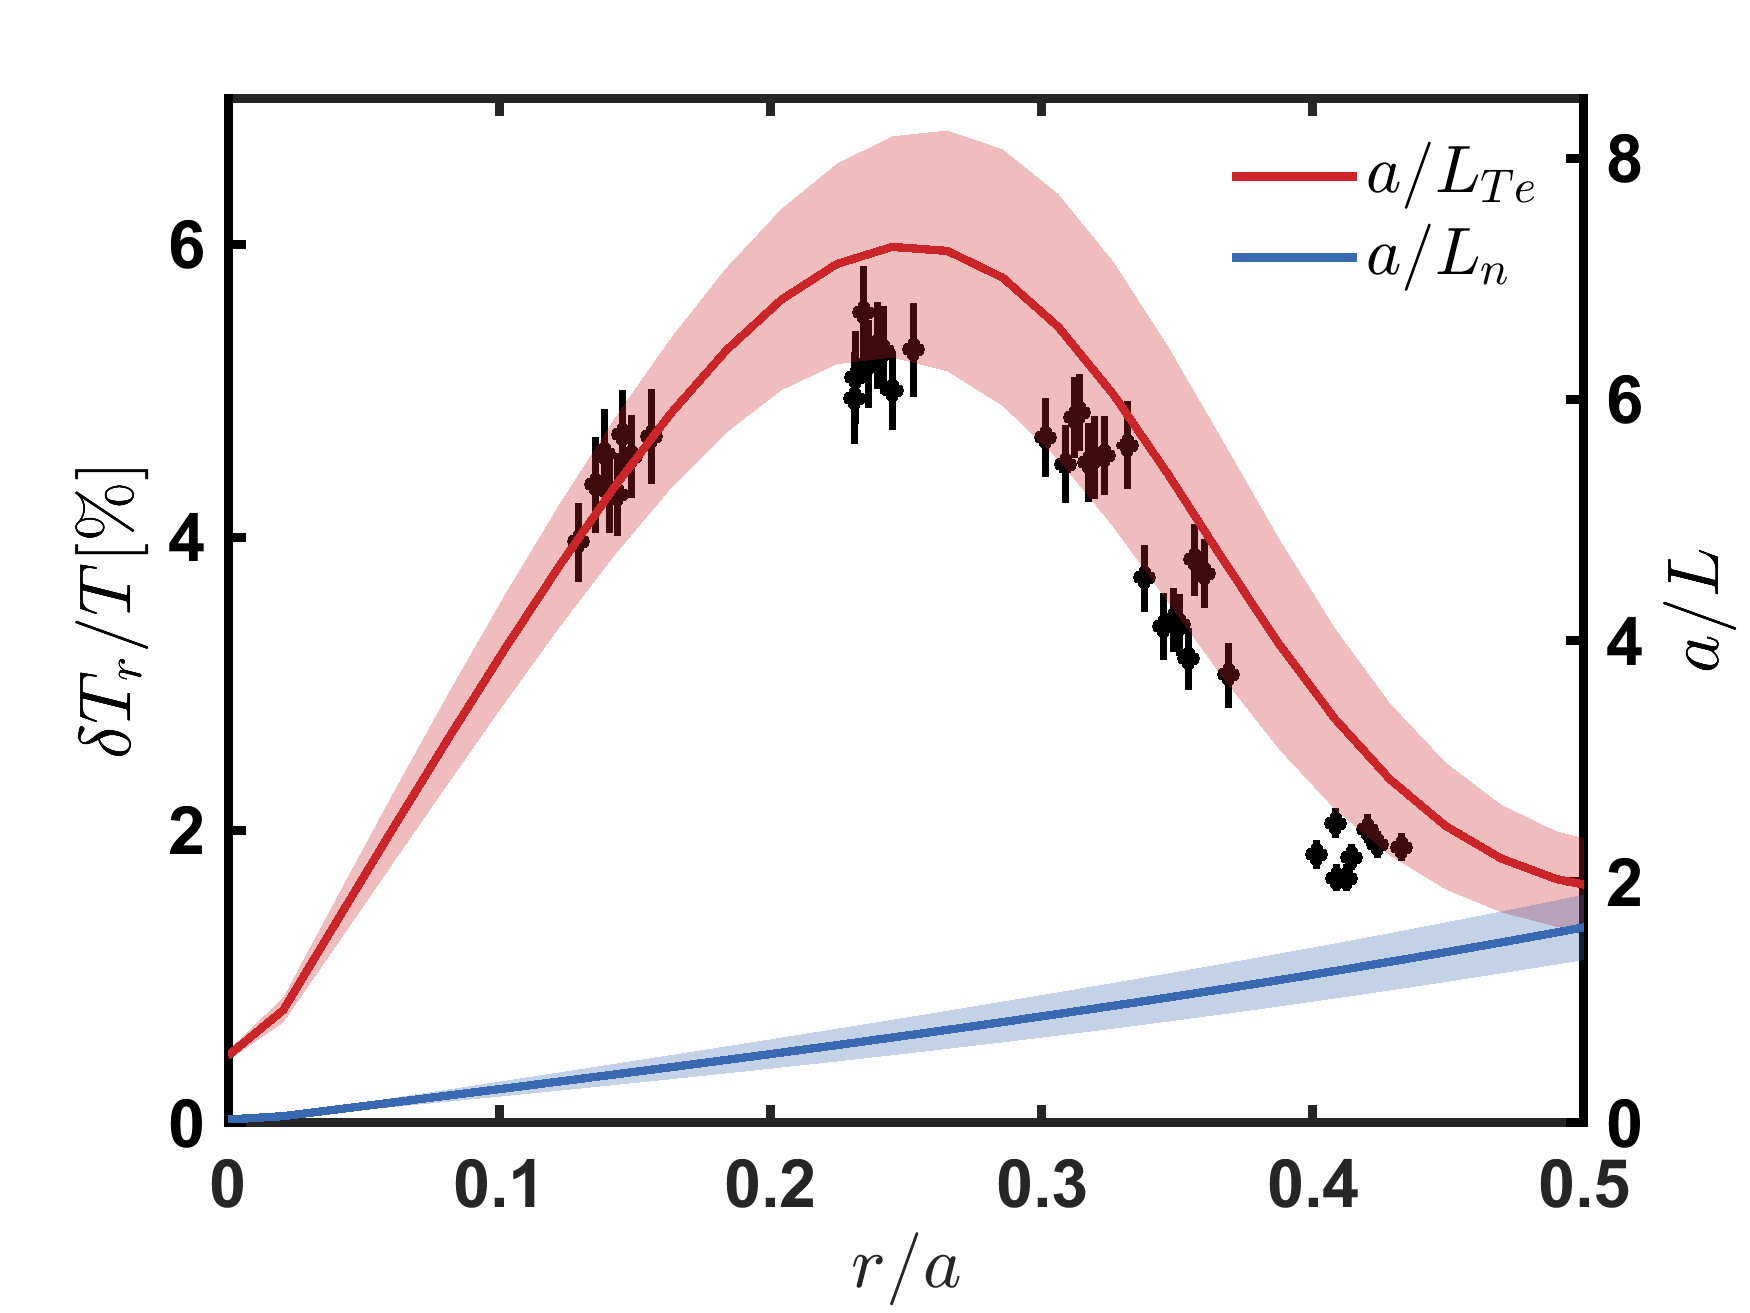
\includegraphics[width=\textwidth]{Figures/ch4_flucs_summary_final.png}}
\end{subfigure}
\hfill
\begin{subfigure}[]{.45\textwidth}
  \centering
  \subfloat[]{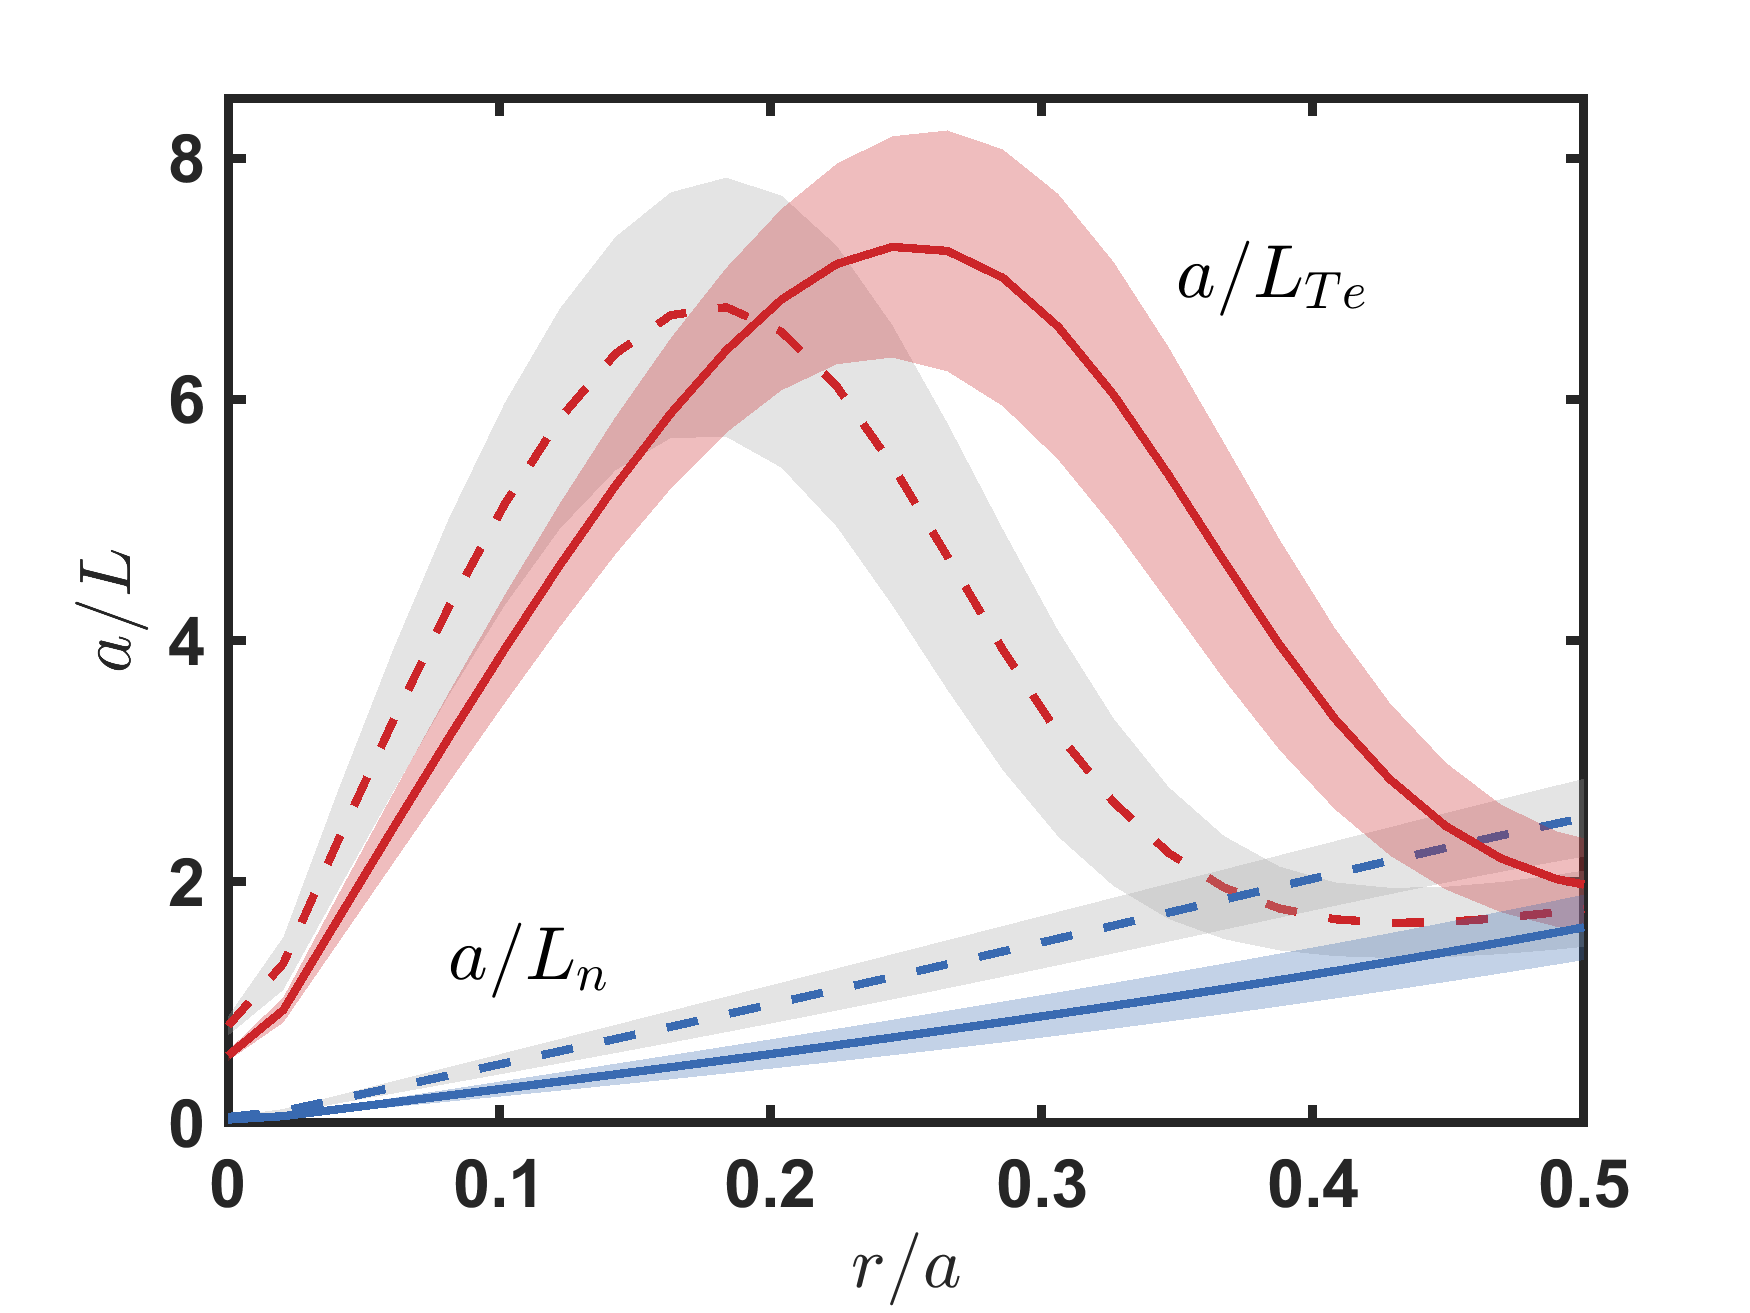
\includegraphics[width=\textwidth]{Figures/ch4_base_case_gradient_scale_length_cmpr.png}}

\end{subfigure}
\hfill
\begin{subfigure}[]{.45\textwidth}
  \centering
  \subfloat[]{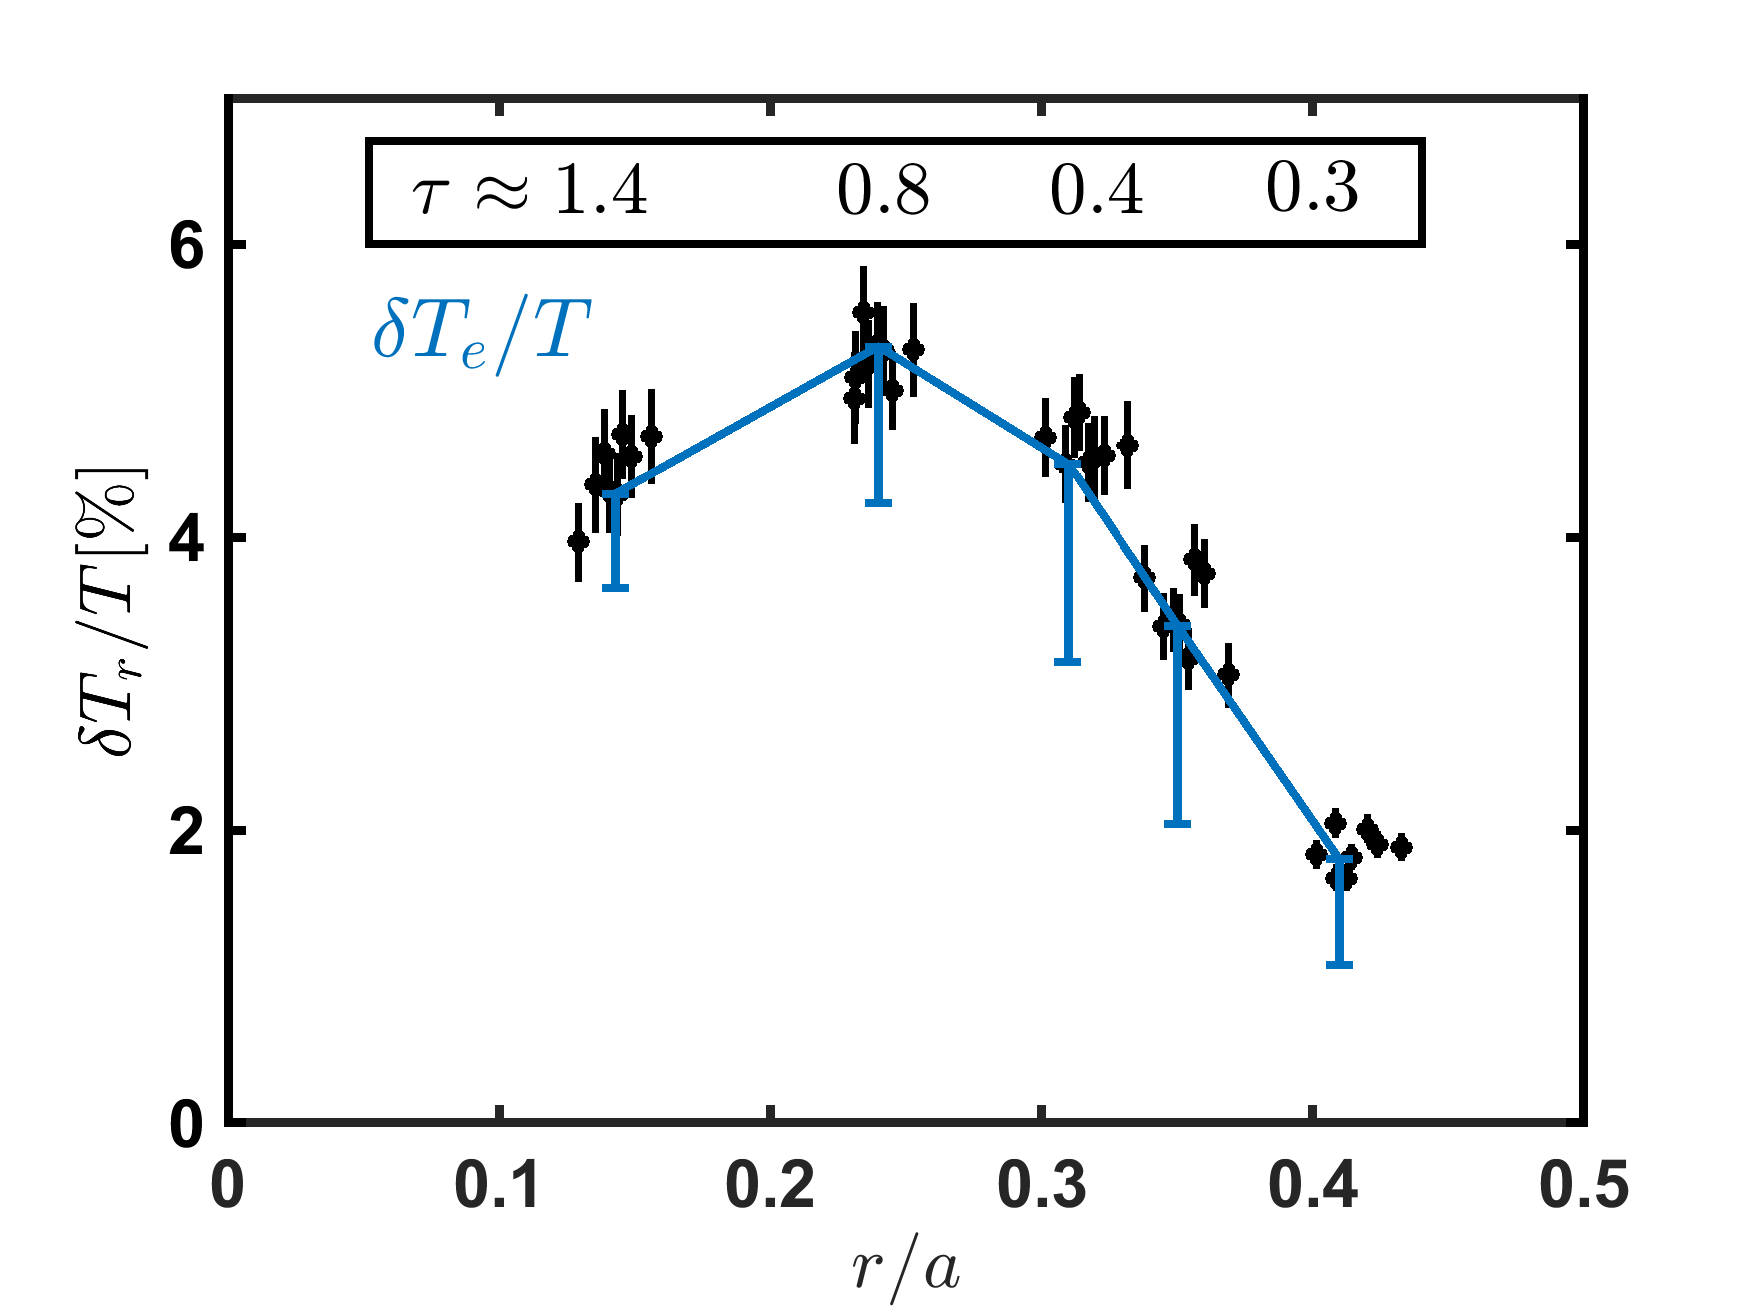
\includegraphics[width=\textwidth]{Figures/ch4_flucs_sys_err.png}}

\end{subfigure}

\caption{MCMC fits to $n_e$ (a) and $T_e$ (b) for high on-axis $T_e$ methane plasma discharge conditions overlaid on the base case profiles. (c) $\delta T_r /T_r$ for each discharge used to generate the profile fits. (d) Comparison of $a/L_n$ and $a/L_{Te}$ with the base case, with the base case uncertainties indicated in gray. (e) The modeled range of $\delta T_e/T_e$  based on the indicated plasma optical depth and assuming a vessel reflectivity of $\Gamma=0.9$.}
\label{fig:methane_fluc_summary}
\end{figure*}

The radial profile of $\delta T_r /T_r$ for high $T_e$ methane plasma conditions is shown in Fig.\ \ref{fig:methane_fluc_summary}(c) with a comparison of $a/L_n$ and $a/L_{Te}$ to those in the base case shown in Fig.\ \ref{fig:methane_fluc_summary}(d). $a/L_n$ is lower in these discharge conditions as compared with the base case, with an approximate range $a/L_n=0.3-1$ in the radial range $0.1 < r/a < 0.4$. $a/L_{Te}$ is larger for $r/a>0.25$. The radial profile of $\delta T_r/T_r$ differs from that of the base case. $\delta T_r/T_r$ decrease from approximately 5\% to 2\% beyond $r/a\approx 0.25$, and this decrease coincides with a decrease in $a/L_{Te}$ from approximately 7 to 2 over the same range. The alignment of the $\delta T_r/T_r$  profile with $a/L_{Te}$ may be interpreted as direct evidence of electron-temperature-gradient-driven core turbulence in these discharge conditions. The corresponding modeled electron temperature fluctuation ranges are shown in Fig.\ \ref{fig:methane_fluc_summary}(e). The minimum predicted $\delta T_e/T_e$  at $r/a\approx0.25$ is above 4\%. Despite relatively high systematic uncertainty, it is clear that like $\delta T_r/T_r$, $\delta T_e/T_e$  is expected to decrease significantly from $r/a\approx0.25$ to $r/a\approx0.4$. Within $r/a\approx0.3$, the $\delta T_e/T_e$  amplitude may be constant. The difference observed in $\delta T_r/T_r$ between these conditions and the base case may be related to methane versus hydrogen fueling, which we now discuss.


\subsection{Profile Matched Hydrogen and Methane Fueled Discharges} \label{sec:h2_vs_ch4_dTr}

\begin{figure*}[!htbp]
\centering
\begin{subfigure}[]{.49\textwidth}
  \centering
  \subfloat[]{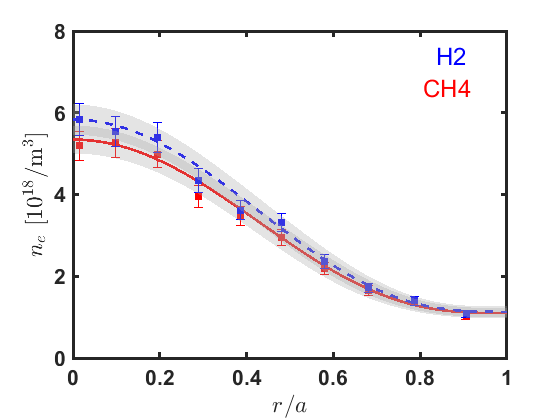
\includegraphics[width=\textwidth]{Figures/ne_ch4_h2_overlay.png}}
\end{subfigure}
\hfill
\begin{subfigure}[]{.49\textwidth}
  \centering
  \subfloat[]{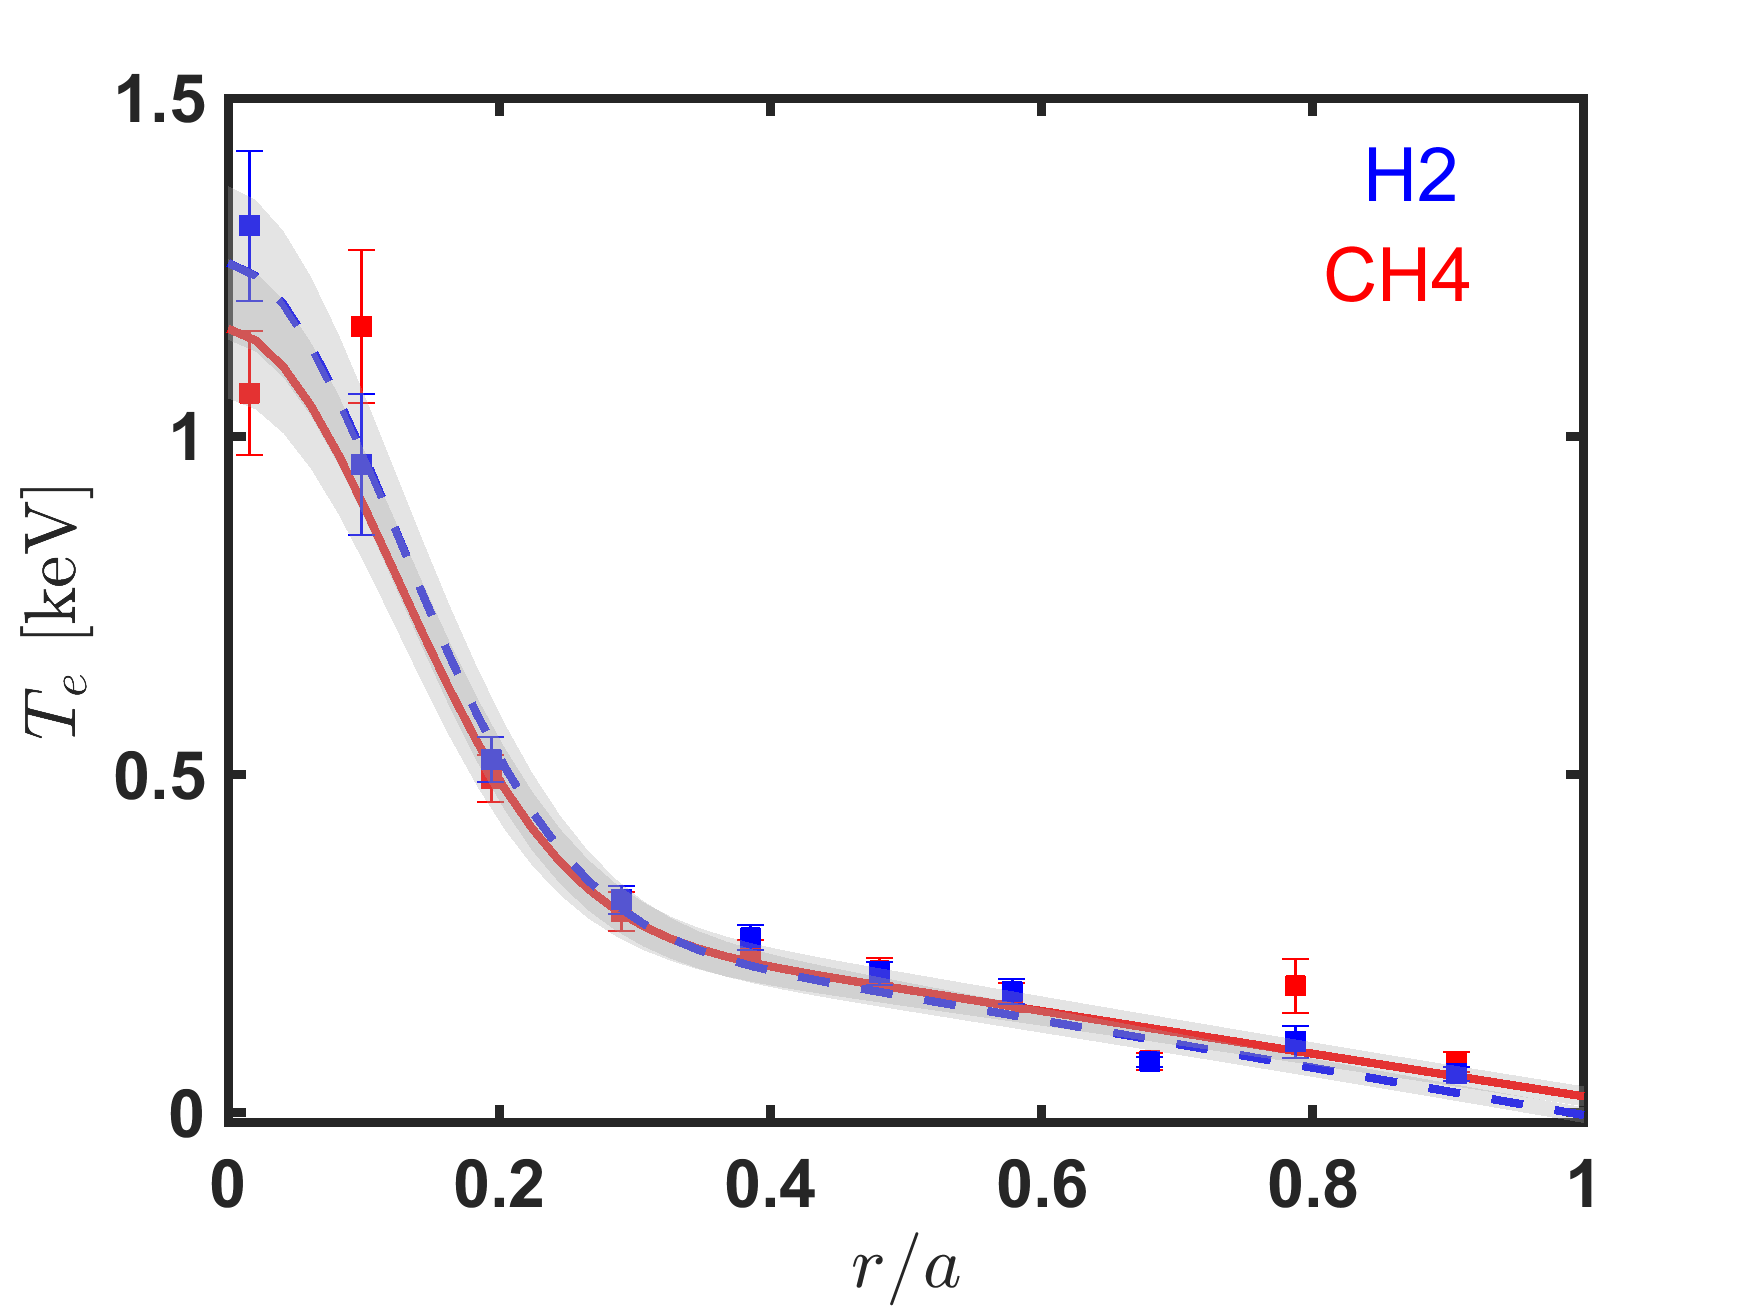
\includegraphics[width=\textwidth]{Figures/Te_ch4_h2_overlay.png}}
\end{subfigure}
\caption{Profiles of electron density (a) and temperature (b) for similar hydrogen and methane discharges with line averaged density $n_e=3.6\times$10\textsuperscript{18}\,m\textsuperscript{-3}.}
\label{fig:h2_vs_ch4_profiles}
\end{figure*}

\begin{figure}[!htbp]
\centering
{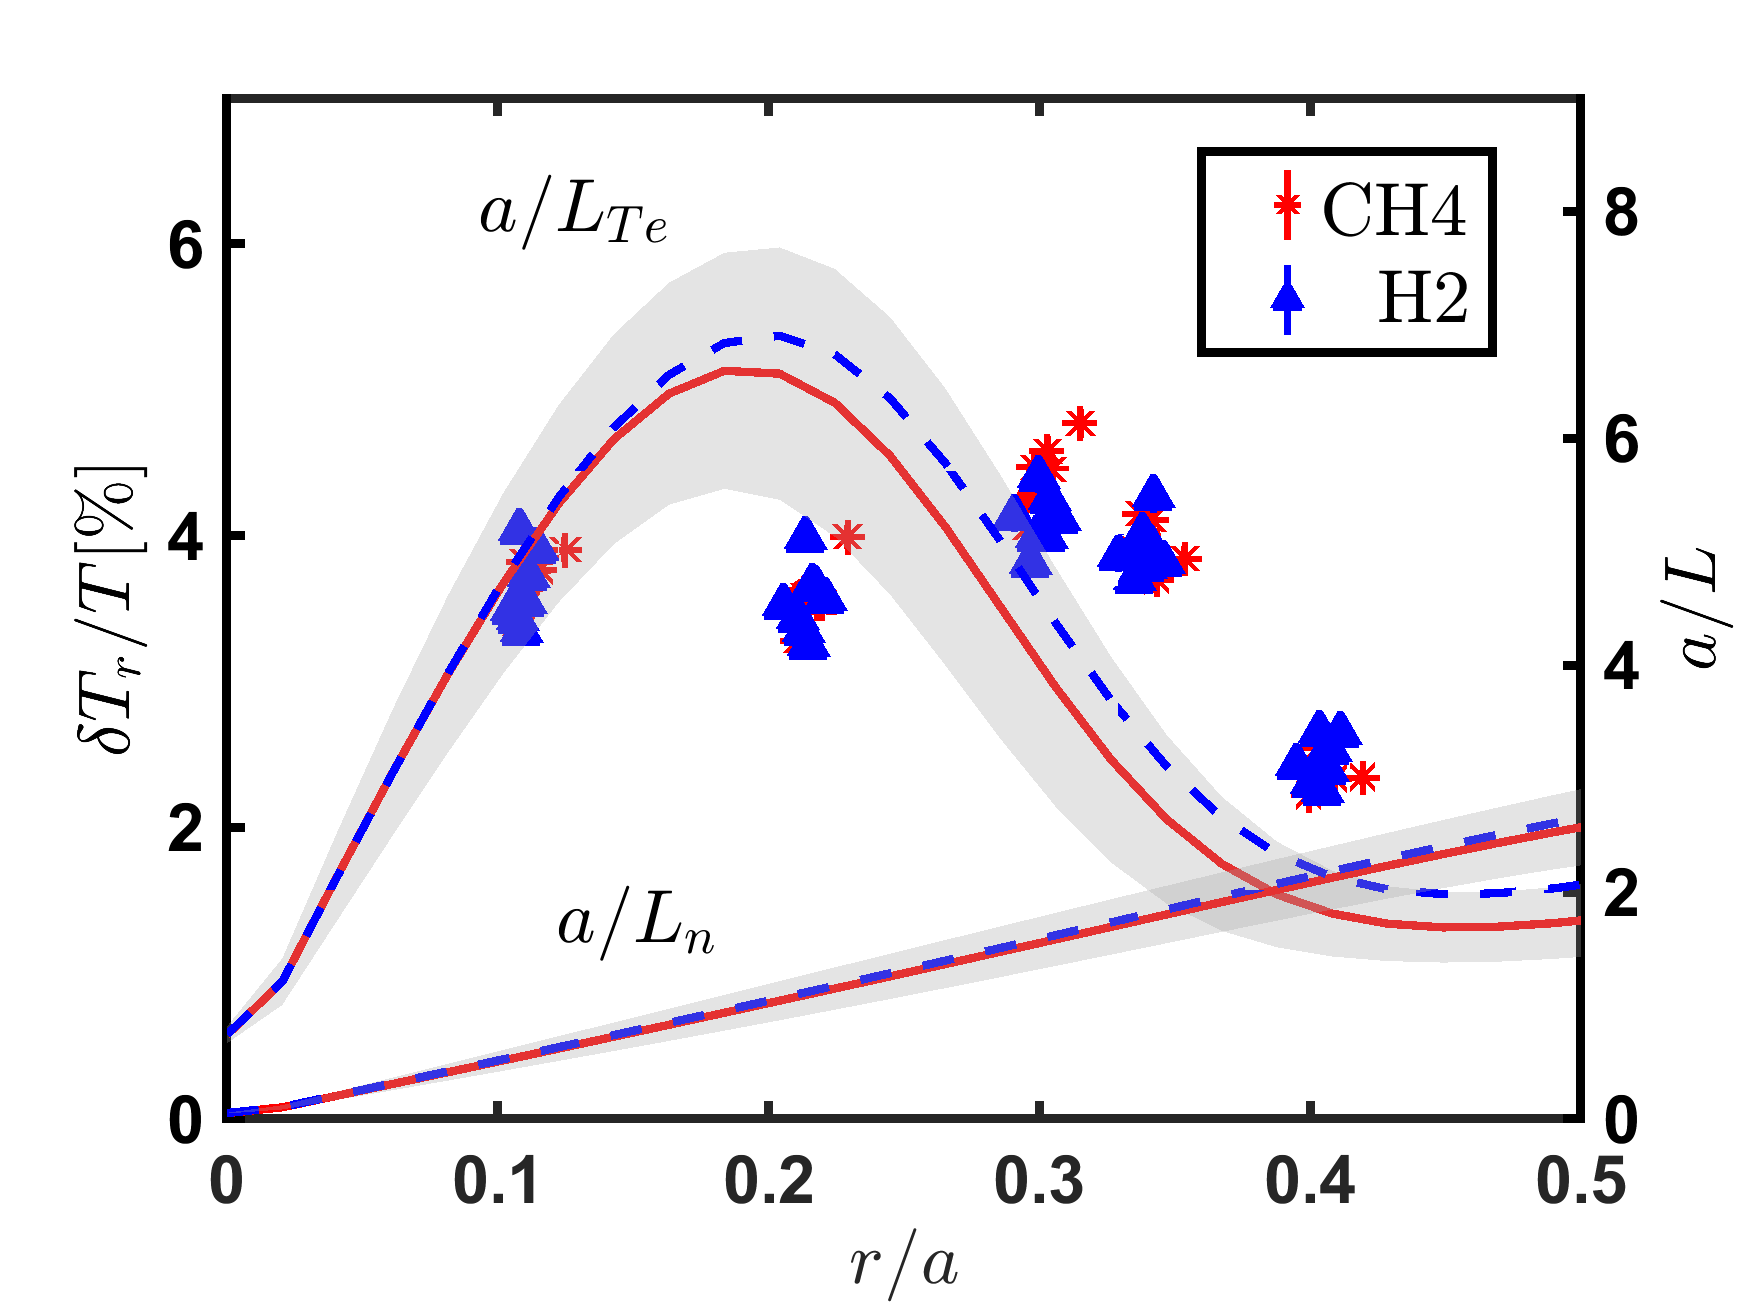
\includegraphics[width=.45\textwidth]{Figures/fluc_ch4_h2_overlay.png}}
\hfill

\caption{Radiation temperature fluctuation profiles for similar methane and hydrogen plasma discharge conditions corresponding to the profiles shown in Fig.\ \ref{fig:h2_vs_ch4_profiles}. Normalized inverse gradient scale lengths are overlaid. The uncertainty in $a/L_n$ and $a/L_{Te}$ is indicated only for methane for clarity, and markers are sized to the vertical error bar.}
\label{fig:h2_ch4_dT_overlay}
\end{figure}

To assess the degree to which a difference in fueling gas may contribute to the discrepancy between $\delta T_r/T_r$ in the base case and high on-axis $T_e$ methane-fueled discharges, we consider now discharge conditions that are well-matched with hydrogen and methane fueling. $n_e$ and $T_e$ profiles are shown for two similar sets of discharge conditions in Fig.\ \ref{fig:h2_vs_ch4_profiles}. The MCMC fits to Thomson scattering data are equivalent within the error bars, as is the raw data, except for the on-axis $T_e$. The line-averaged density for both ensembles is $n_e=3.6\times$10\textsuperscript{18}\,m\textsuperscript{-3}. Absorbed power inferred from the diamagnetic loop is in agreement, with $P_{\mathrm{abs}}=13.1\pm 1.8$\,kW in H\textsubscript{2} and $P_{\mathrm{abs}}=13.1 \pm 1.6$\,kW in CH\textsubscript{4}. $\delta T_r/T_r$ profiles are compared for these discharge conditions in Fig.\ \ref{fig:h2_ch4_dT_overlay}.

The radiation temperature fluctuation profile in both H\textsubscript{2} and CH\textsubscript{4} discharge conditions with well-matched profiles agree within the accessible measurement range. The apparent difference in $a/L_{Te}$ between the discharges is not resolvable within the error bars on the MCMC fit. The $\delta T_r/T_r$ profile in both plasmas is similar to the base case, Fig.\ \ref{fig:base_case_summary}. Given the consistency of the profiles and gradients, as well as line-averaged density and absorbed power, the agreement in $\delta T_r/T_r$ provides evidence that the difference seen between CECE measurements in the high $T_e$ methane discharges compared to the base case is unlikely explained solely by a difference in fueling gas.






%%%%%%%%%%%%%%%%%%%%%%%%%%%%%%%%%%%%%%%%%%%%%%%%%%%%%%%%%%%%%%%%%%%%%%%%%%%%%%%%%%%%%%%%%%%%%%%%%%%%%%%%%%%%%%%%%%%%%%
% Database results -- would really like to add data to more expansive result if showing this!

\section{A Database Study of $\delta T_r/T_r$ in QHS Plasmas} \label{sec:dT_database}

The combination of simultaneously co-varying $a/L_n$ and $a/L_{Te}$, and the modification of $\delta T_r/T_r$ by $\delta n/n$, makes an assessment of the driving gradient dependence of core fluctuation amplitudes difficult with only the radial profiles shown in Section \ref{sec:exp_cece}. However, such an assessment is important for identifying possible core instability mechanisms, as pressure gradients drive drift-wave instabilities \cite{horton1999drift}. A database of CECE measurements has been compiled using the measurements presented in Section \ref{sec:exp_cece} and additional discharges. Each entry in this database is a set of CECE measurements for a given discharge, and sets of discharges are grouped to form ensembles for generating MCMC Thomson scattering fits. The database can be quickly regenerated with various spectral analysis settings. The broadband fluctuation amplitude is determined by integrating the spectrum within 20-200\,kHz, and the noise coherence is defined as the average real part of the complex coherence in 200-250\,kHz ($[f_1,f_2,f_3,f_4] = [20,200,200,250]$\,kHz in Eq.\ \eqref{eq:M3}). This is equivalent to the analysis methodology used in Section \ref{sec:exp_cece}. The database enables simple filtering of measurements by e.g.\ the radial position of the fluctuation measurement and a range of normalized inverse gradient scale lengths.

%In light of the complications with measurements at low plasma density in HSX (Chapter 2), the database results shown here correspond to measurements in plasmas with line-averaged density greater than $n_e=3\times$10\textsuperscript{18}\,m\textsuperscript{-3}.

\begin{figure*}[!htbp]
\centering
\begin{subfigure}[]{.49\textwidth}
  \centering
  \subfloat[]{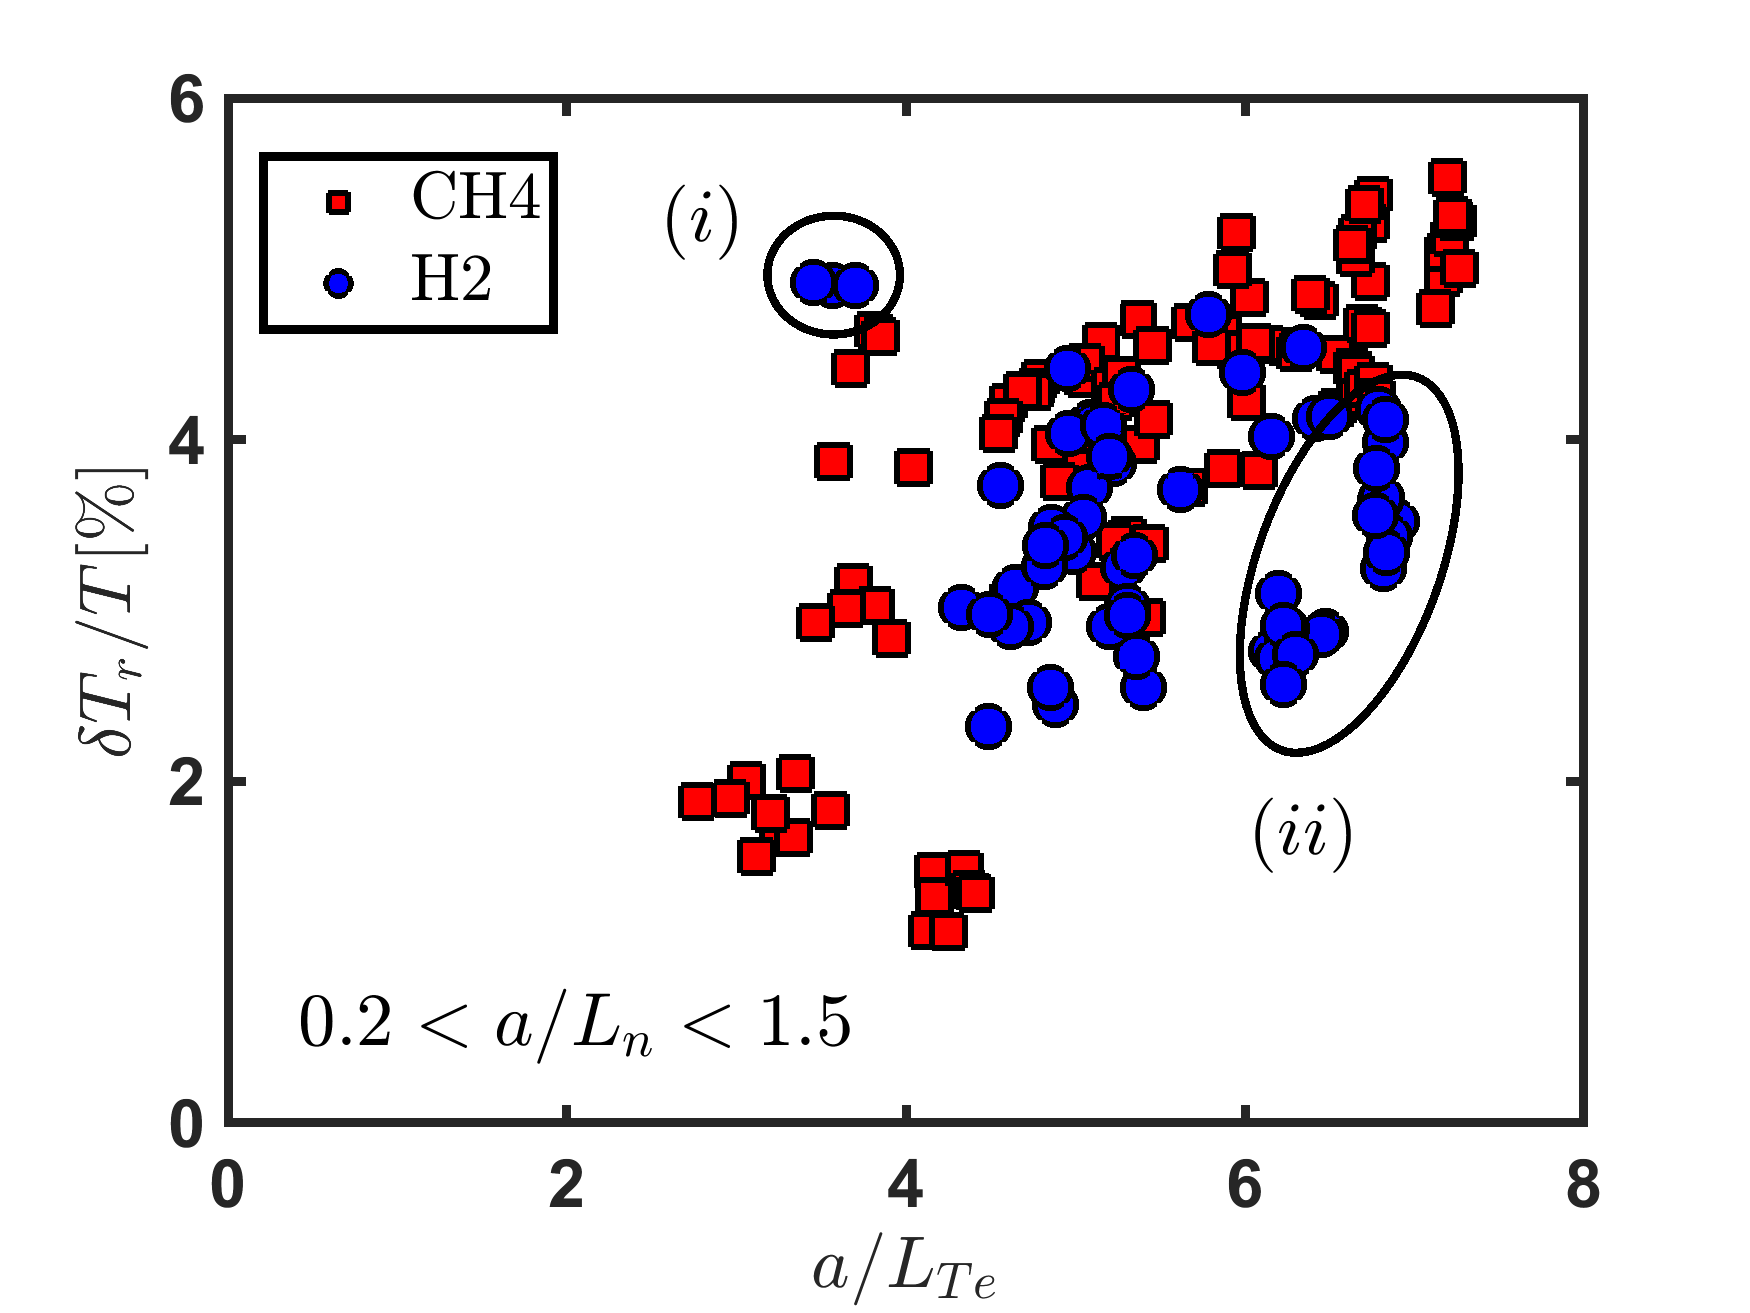
\includegraphics[width=\textwidth]{Figures/dB_omte_a_annotated2.png}}
\end{subfigure}
\hfill
\begin{subfigure}[]{.49\textwidth}
  \centering
  \subfloat[]{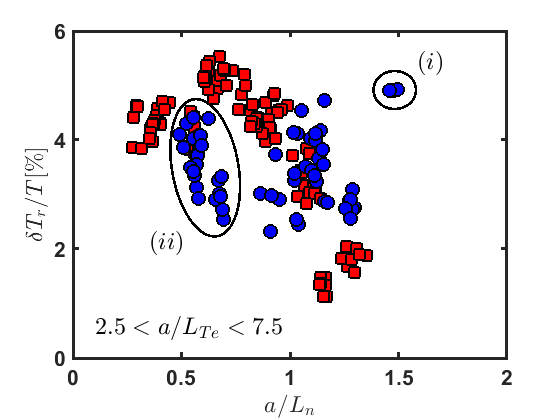
\includegraphics[width=\textwidth]{Figures/dB_omne_b_annotated2.png}}
\end{subfigure}
\hfill
\begin{subfigure}[]{.49\textwidth}
  \centering % TODO: consider removing line?
  \subfloat[]{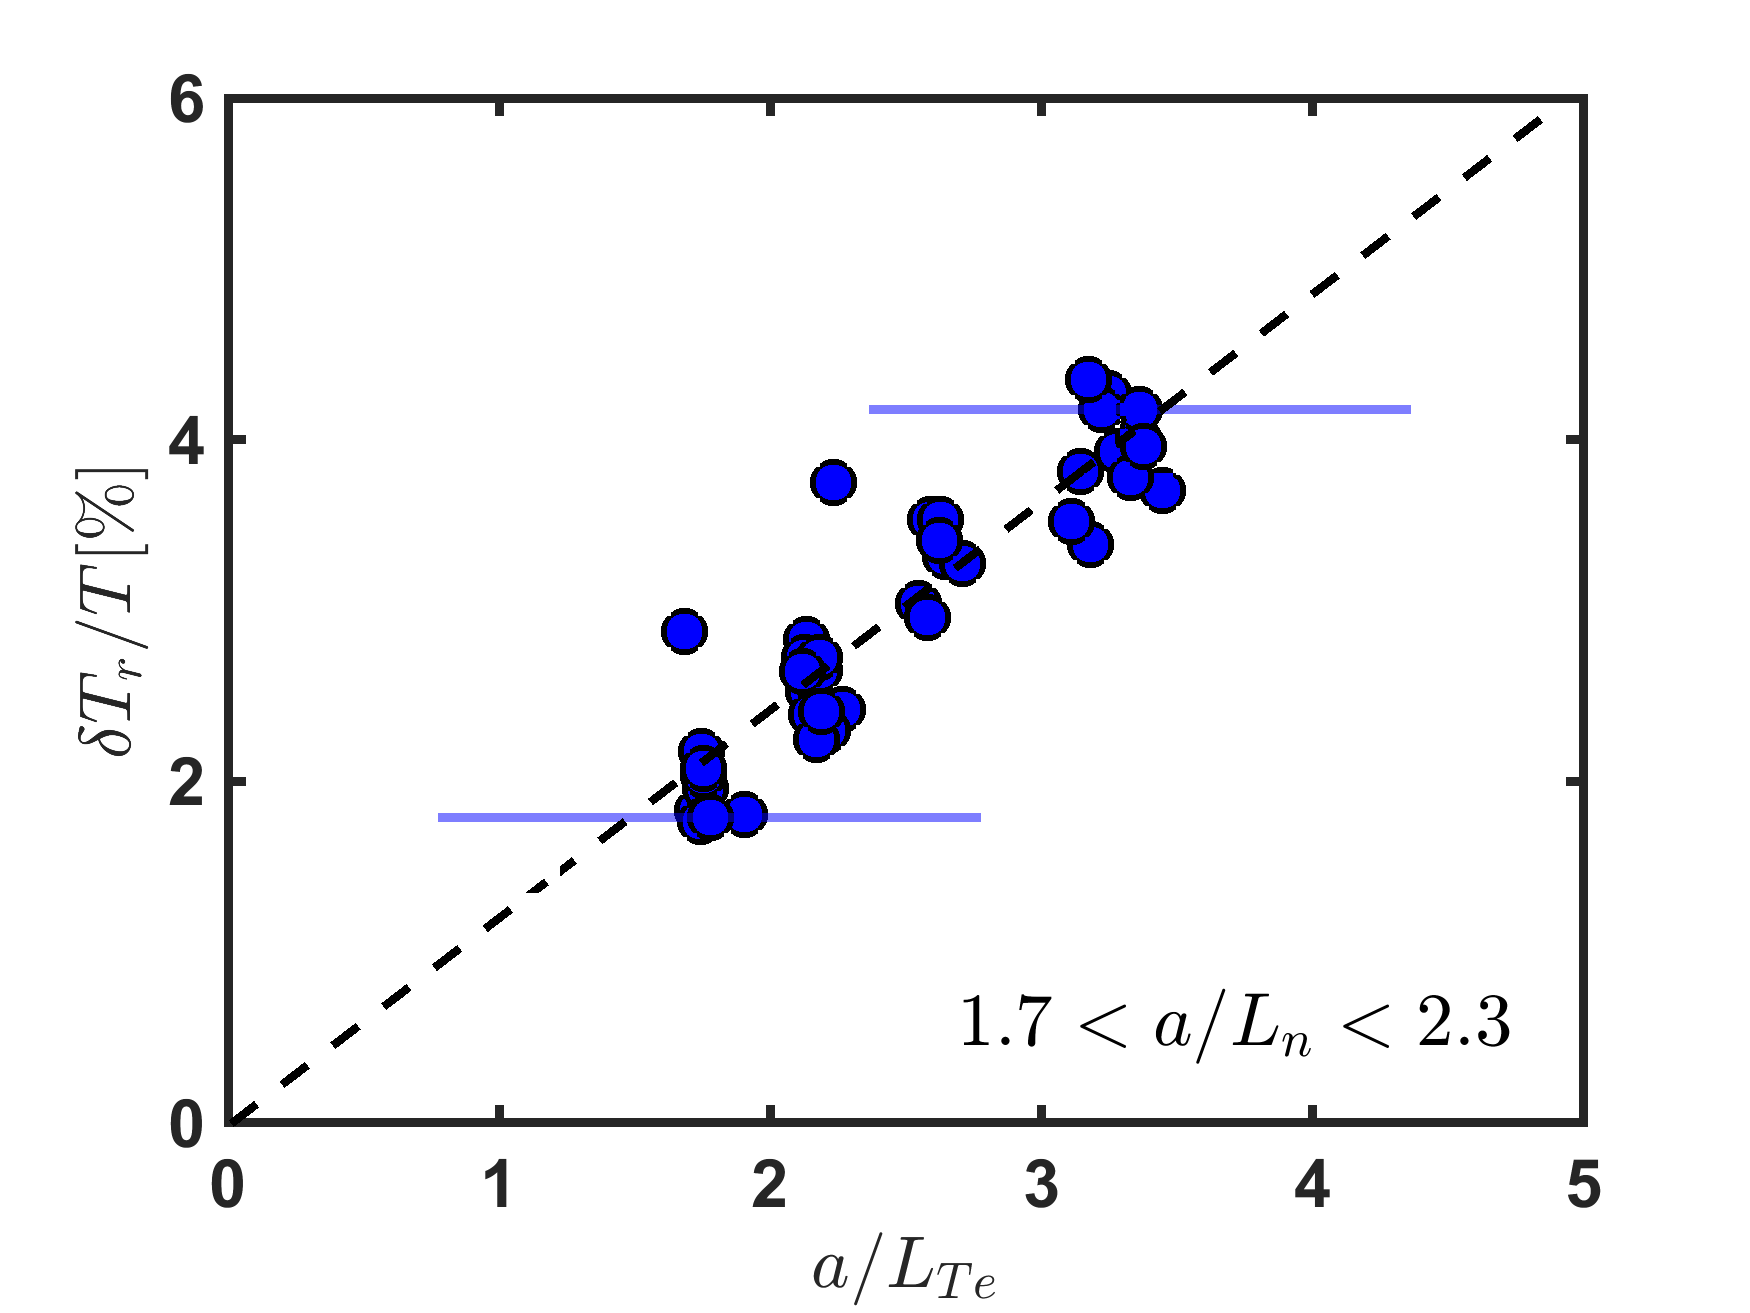
\includegraphics[width=\textwidth]{Figures/limdB_omte_c_tighter_line.png}}
\end{subfigure}
\begin{subfigure}[]{.49\textwidth}
  \centering
  \subfloat[]{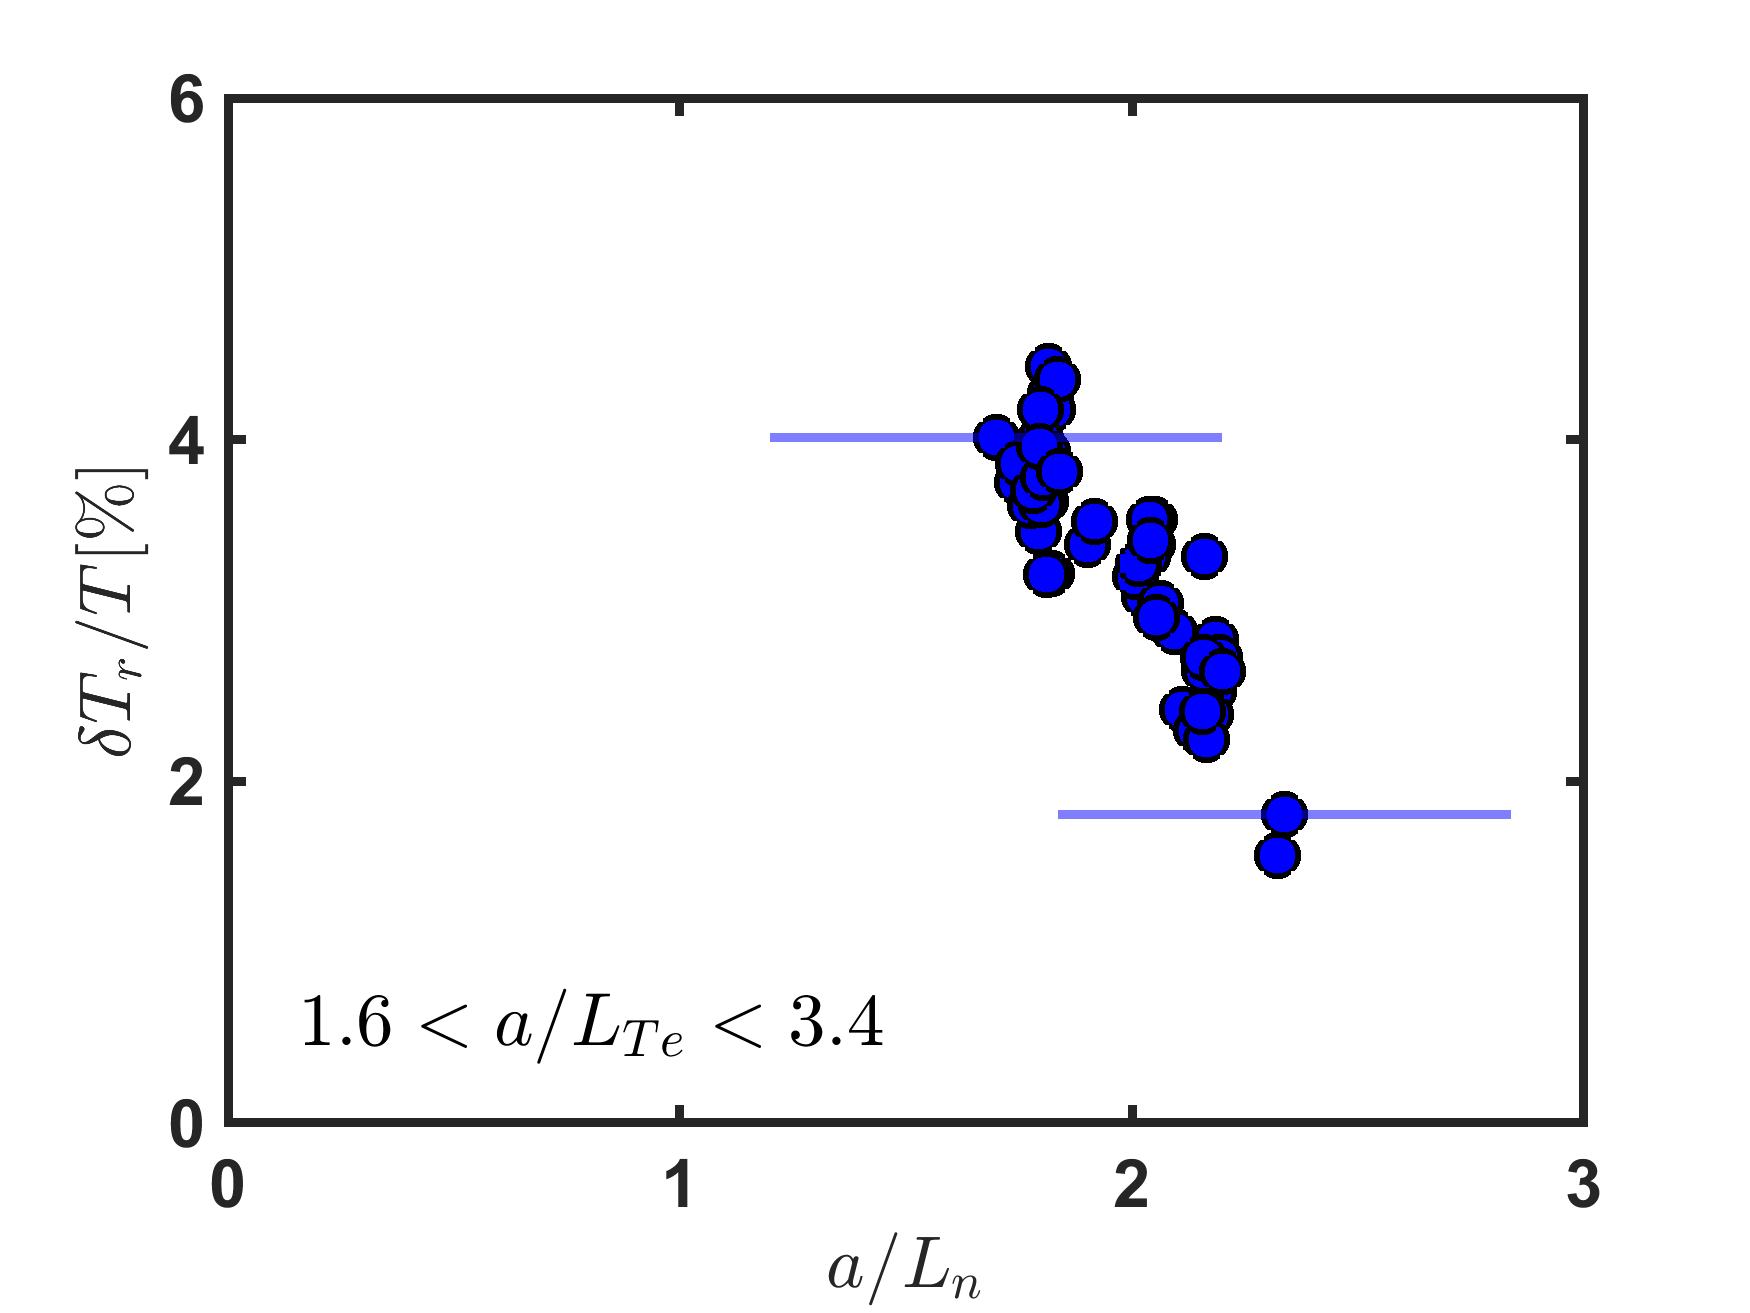
\includegraphics[width=\textwidth]{Figures/limdB_omn_d_tighter_err.png}}
\end{subfigure}

\caption{Database of $\delta T_r/T_r$  derived from CECE measurements within $0.1 < r/a < 0.4$. The top row (a-b) is comprised of measurements filtered for $a/L_n<1.5$, with the corresponding $a/L_{Te}$ range shown in (b). Two regions, (i) and (ii), referred to in the text are shown. The bottom row (c-d) consists of measurements filtered to a tight range about $a/L_n=2$. Representative uncertainties in $a/L_n$ and $a/L_{Te}$ are $\pm 0.5$ and $\pm 1$, respectively. These are shown for two points in the bottom row. The uncertainty in $\delta T_r/T_r$ is approximately within the markers for H\textsubscript{2} measurements, and the relative uncertainty in CH\textsubscript{4} measurements is approximately 10\%. A best-fit line to the $\delta T_r/T_r$ amplitude is shown in (c). }
\label{fig:full_db}
\end{figure*}

A database scaling of $\delta T_r /T$ with $a/L_n$ and $a/L_{Te}$ is shown for on-axis heated QHS configuration plasmas in Fig.\ \ref{fig:full_db} for measurements within $0.1<r/a<0.4$. Plasmas with minimum line average density of $n_e=3\times$10\textsuperscript{18}\,m\textsuperscript{-3} are represented. Measurements in regions with optical depth $\tau<0.2$ are excluded, as they are in Section \ref{sec:exp_cece}, based on the discussion of systematic uncertainty in Section \ref{sec:sys_error}. Measured fluctuations are in the approximate range $\delta T_r /T_r = 1.5 - 6\%$. The sensitivity level is $1.5\%$ except in the outermost channel pair, where it is $1.2\%$ due to higher channel IF bandwidth (see Eq.\ \eqref{eq:thermnoise-corr}); measurements shown below 1.5\% correspond to this outermost channel pair. Error bars are not displayed for readability in the top row, but are shown for two points in the bottom row. Representative uncertainty in $a/L_n$ is $\pm0.5$ and in $a/L_{Te}$ is $\pm1$. The relative statistical uncertainty in $\delta T_r/T_r$ is approximately 5\% in H\textsubscript{2} discharges, which is within the markers. The stationary phase was somewhat lower in duration for the CH\textsubscript{4} discharges, and representative relative uncertainties are approximately 10\%.

Fig.\ \ref{fig:full_db}(a) shows the scaling of $\delta T_r/T_r$ with $a/L_{Te}$ for measurements in the range $a/L_n < 1.5$, with $a/L_n=0.2$ corresponding to the minimum in the tabulated database. With these constraints on the analysis, there is not an apparent trend in the fluctuation amplitude with $a/L_{Te}$ in hydrogen-fueled discharges that is evident in Fig.\ \ref{fig:full_db}(a). In contrast, the fluctuation amplitude is well-correlated with $a/L_{Te}$ in methane-fueled discharges. This is not to rule out a scaling of $\delta T_r/T_r$  with $a/L_{Te}$ in H\textsubscript{2} plasmas: Fig.\ \ref{fig:full_db}(b) shows that the two outlier points in H\textsubscript{2} plasmas at lowest $a/L_{Te}$, indicated as region (i), occur at the highest values of $a/L_n$. Likewise, region (ii) occurs at the minimum $a/L_n$ for H\textsubscript{2} discharges. The set of measurements excluding regions (i) and (ii), while not spanning as large a range of $a/L_{Te}$, exhibits a similar trend as measurements in CH\textsubscript{4} discharges. Regarding the $a/L_n$ scaling of the measurements in Fig.\ \ref{fig:full_db}(b), there is not a clear trend in H\textsubscript{2} discharges, while higher $\delta T_r/T_r$ is associated with lower $a/L_n$ for $a/L_n > 0.5$ in CH\textsubscript{4} discharges. That $\delta T_r/T_r$ are similar in the cluster of points below $a/L_n=0.5$ and the cluster near $a/L_n=1$  in CH\textsubscript{4} discharges may suggest that $\delta T_r/T_r$ is associated with higher $a/L_{Te}$ rather than a lower $a/L_n$.

A database comprising a narrower range of measurements at approximately $a/L_n=2$ is shown in Fig.\ \ref{fig:full_db}(c-d). This result is compared with nonlinear gyrokinetic predictions of $\delta T_r/T_r$ in Section \ref{sec:gk_omt_scan}. The exact choice of the $a/L_n$ filter was made to balance competing goals of matching the gyrokinetic simulation $a/L_n$ input and having a reasonable number of measurements ($N=33$ here). With these constraints, Fig.\ \ref{fig:full_db}(c) shows a clear trend of the fluctuation amplitude with $a/L_{Te}$. Unlike the data in Fig.\ \ref{fig:full_db}(a-b), the uncertainty in $a/L_n$ (approximately $\pm0.5$) is nearly equal to the range of $a/L_n$ considered, and the apparent trend in Fig.\ \ref{fig:full_db}(d) may not be meaningful. On the other hand, the data comprise a sufficiently large range of $a/L_{Te}$ that the trend is expected to be robust to the relatively high uncertainty in $a/L_{Te}$ (approximately $\pm1$). Filtering the database in a narrow range of $a/L_{Te}$ in hydrogen plasmas produces only scatter in $a/L_n$, suggesting that the apparent association of $\delta T_r/T_r$  with lower values of $a/L_n$ may be artificial.

\begin{figure}[!htbp]
  \centering
  {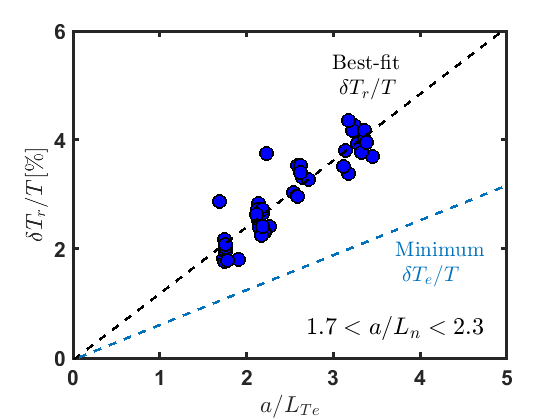
\includegraphics[width=.45\textwidth]{Figures/dB_dTe.png}}
\hfill

\caption{The database result shown in Fig.\ \ref{fig:full_db}(c) with a modeled minimum $\delta T_e/T_e$ best-fit line shown in light blue. The best-fit line is derived using the average optical depth over all measurements, $\tau\approx0.4$, and assuming an effective vessel reflectivity of $\Gamma=0.9$.}
  \label{fig:dB_dTe}
\end{figure}

With knowledge of the plasma optical depth, a range of possible $\delta T_e/T_e$  can be modeled from measured $\delta T_r/T_r$. The data in Fig.\ \ref{fig:full_db}(c) are shown with a corresponding best-fit line to the minimum $\delta T_e/T_e$ amplitude in Fig.\ \ref{fig:dB_dTe}. Here, the average optical depth over all measurements, $\tau\approx0.4$, is used assuming a vessel reflectivity $\Gamma=0.9$. Despite the relatively large range of possible $\delta T_e/T_e$, which is between the indicated minimum $\delta T_e/T_e$ and $\delta T_r/T_r$ best-fit lines, there is a clear trend in the electron temperature fluctuation amplitude with $a/L_{Te}$. If the vacuum vessel reflectivity is closer to unity, which is empirically true based on ECE profile measurements in HSX, then the $\delta T_e/T_e$ trend is closer to that of $\delta T_r/T_r$.


In HSX, trapped electron modes (TEMs) are expected to limit confinement, except possibly electron temperature gradient modes within $r/a\approx0.2$, as discussed in Section \ref{sec:hsx_turbo_review}. The CECE diagnostic primarily resolves modes with poloidal wavenumbers $k_\theta < 2.1$\,cm\textsuperscript{-1} and radial wavenumbers $k_r < 6.3$\,cm\textsuperscript{-1}. For the discharges considered in the previous section and in the compiled database, $T_e$ in the region accessible to CECE varies in the approximate range 0.3-1.5\,keV. The normalized wavenumber sensitivity at 0.3\,keV is $k_\theta \rho_s \lesssim 0.35$ and at 1.5\,keV is $k_\theta \rho_s \lesssim 0.75$. In either range, TEMs are predicted to be the dominant instability, with electron temperature gradient modes typically dominant at $k_\theta \rho_s > 1$. Therefore, CECE is expected to be sensitive primarily to TEM turbulence in HSX. The scaling shown in Fig.\ \ref{fig:dB_dTe} suggests that TEMs are driven by the electron temperature gradient within the mid-radius of HSX.


%%%%%%%%%%%%%%%%%%%%%%%%%%%%%%%%%%%%%%%%%%%%%%%%%%%%%%%%%%%%%%%%%%%%%%%%%%%%%%%%%%%%%%%%%%%%%%%%%%%%%%%%%%%%%%%%%%%%%%
\section{\label{sec:gkcompare} Synthetic Fluctuation Data and Comparison with Experimental Results}
%%%%%%%%%%%%%%%%%%%%%%%%%%%%%%%%%%%%%%%%%%%%%%%%%%%%%%%%%%%%%%%%%%%%%%%%%%%%%%%%%%%%%%%%%%%%%%%%%%%%%%%%%%%%%%%%%%%%%%
% Introduction and description of synthetic diagnostic below

%%%%%%%%%%%%%%%%%%%%%%%%%%%%%%%%%%%%%%%%%%%%%%%%%%%%%%%%%%%%%%%%%%%%%%%%%%%%%%%%%%%%%%%%
\subsection{A Synthetic CECE Diagnostic} \label{sec:synth_diag}
Meaningful comparisons of experimental turbulence measurements with numerical simulation may require the use of synthetic diagnostics to mimic the measurement properties of an experimental diagnostic. A synthetic diagnostic refers to software used to process numerical data, in this case from a nonlinear gyrokinetic simulation of plasma turbulence, into a signal that can be compared directly with experimental measurements. A synthetic CECE diagnostic developed by Gavin Held as part of an ongoing thesis project is used in this work. This synthetic diagnostic is based on the implementation described in \cite{holland2009implementation}.

\begin{figure}[!htbp]
  \centering
  {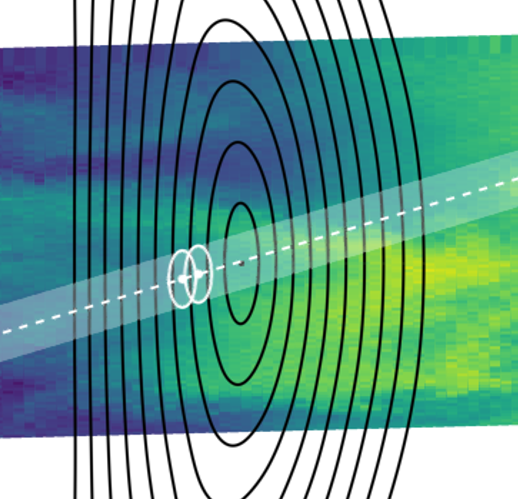
\includegraphics[width=.45\textwidth]{Figures/very_cropped_cece_overlay_fig.png}}
\hfill

\caption{CECE synthetic diagnostic schematic showing the $1/e$ envelope of the Gaussian point spread function (white ovals) centered along the HSX CECE diagnostic line of sight (dashed white line). Flux surfaces in a helical cut of the HSX boxport are shown as black lines, with the coloring indicating a fluctuating signal output from a nonlinear \gene{} simulation. Figure courtesy of Gavin Held.}
  \label{fig:emiss_to_synth_chans}
\end{figure}

The synthetic diagnostic generates a time series of a fluctuating quantity from \gene{} data. The required inputs include nonlinear simulation output, specification of the magnetic field and ECE sample volume geometry, and the plasma radial electric field $E_r$. The radial electric field is used to transform the simulation data into the lab frame. The ECE geometry is specified by a central channel location $(R_0,Z_0,\zeta_0)$ and corresponding sample volume widths $(L_R,L_Z,L_\zeta)$ determined by the radiometer front-end and the fundamental emission process, as modeled using 3D raytracing and Gaussian quasi-optics. Here, $(R,Z,\zeta)$ can be identified with $(x,y,z)$ appearing in Eq.\ \eqref{eq:Bxyz} in the HSX boxport. Each channel is modeled using an ellipsoidal Gaussian envelope transfer function referred to as a point spread function (PSF),
\begin{align}
	\psi_{\mathrm{PSF}}(R,Z,\zeta) &= \\ &{}\exp\left\{ - \frac{1}{2} \left[ \left(\frac{R-R_0}{L_R}\right)^2 + \left(\frac{Z-Z_0}{L_Z}\right)^2 + \left(\frac{\zeta-
	\zeta_0}{L_\zeta}\right)^2 \right] \right\}. \label{eq:psf}
\end{align}
A schematic showing a PSF overlaid on HSX flux surfaces is shown in Fig.\ \ref{fig:emiss_to_synth_chans}. $L_Z \approx 1.5$\,cm is specified by the ECE beam power radius. Note that $L_Z$ describes the poloidal extent of the sample volume which is vertical in Fig.\ \ref{fig:emiss_to_synth_chans} because the flux surfaces have been rotated. The toroidal extent of the ECE sample volume is approximately equivalent to the poloidal extent for the radiometer front-end design at HSX, $L_Z\simeq L_\zeta$. The radial channel extent is specified by the natural linewidth of emission. $L_R\approx 0.5$\,cm is representative of high-field side channels in HSX for the measurements compared with synthetic data in this chapter.  

A synthetic time trace of the fluctuating signal $S_{\mathrm{synth}}(t)$ is determined by volume integrating the PSF weighted raw signal $S_{\mathrm{lab}}$,
 \begin{align}
 	S_{\mathrm{synth}}(t) = \frac{\int dV S_{\mathrm{lab}}(R,Z,\zeta,t)\psi_{\mathrm{PSF}}(R,Z,\zeta)}{\int dV \psi_{\mathrm{PSF}}(R,Z,\zeta)}, \label{eq:synth_int}
 \end{align}
 where $S_{\mathrm{lab}}$ is the $E \times B$ Doppler shifted raw \gene{} data. The integration is performed using a Monte Carlo method for computational efficiency. The convergence properties of the synthetic diagnostic have been investigated in \cite{anna-bs}.

% \begin{figure}[t]
% \centering
%   {\includegraphics[width=0.7\textwidth]{Chapters/4_ch4_figs/pngs/psf_vs_raw_time_trace.png}}
% \hfill
% \caption{Time trace of the perpendicular component of electron temperature fluctuations with and without processing by the synthetic diagnostic. The synthetic signal here is derived using a point spread function with $L_R=0.5$\,cm and $L_Z=L_\zeta=1.5$\,cm.}
% \label{fig:synth_sigs_unfilt_filt}
% \end{figure}

%\subsubsection*{Finite Sample Volume Effects} \label{sec:sample_volume}
The ECE sample volume fundamentally determines the measured spectrum of radiation temperature fluctuations. Modes with wavelengths smaller than a characteristic channel width are averaged out, while those larger than a characteristic channel width contribute to the measured spectrum \cite{ross1991dispersion,bravenec_wootton_spatial}. In other words, the measured turbulent signal is low-pass filtered in wavenumber such that a larger channel will in general measure a more attenuated spectrum and a correspondingly lower fluctuation amplitude. This effect is captured by the synthetic diagnostic with the PSF transfer function, Eq.\ \eqref{eq:psf}. The time trace of unfiltered \gene{} simulation output and a filtered synthetic signal for a single ECE channel is shown in Fig.\ \ref{fig:synth_sigs_unfilt_filt}. The unfiltered data here refers to the limit of setting the PSF to a Delta function at the center of the flux tube. The PSF dimensions are the experimental beam power radius and natural linewidth. As compared with the raw data, the PSF-filtered synthetic signal is smoother, due to the attenuation of high-frequency modes, and is significantly lower in magnitude. Here, the perpendicular component of the fluctuations $\delta T_{e \perp}/T$ is shown, as this is the component that CECE is primarily sensitive to \cite{hartfuss1996temperature}. In the remainder of this chapter, $\delta T_e/T_e$ refers to $\delta T_{\perp e}/T$.

\begin{figure*}[!htpb]
\centering
\begin{subfigure}[]{.49\textwidth}
  \centering
  \subfloat[]{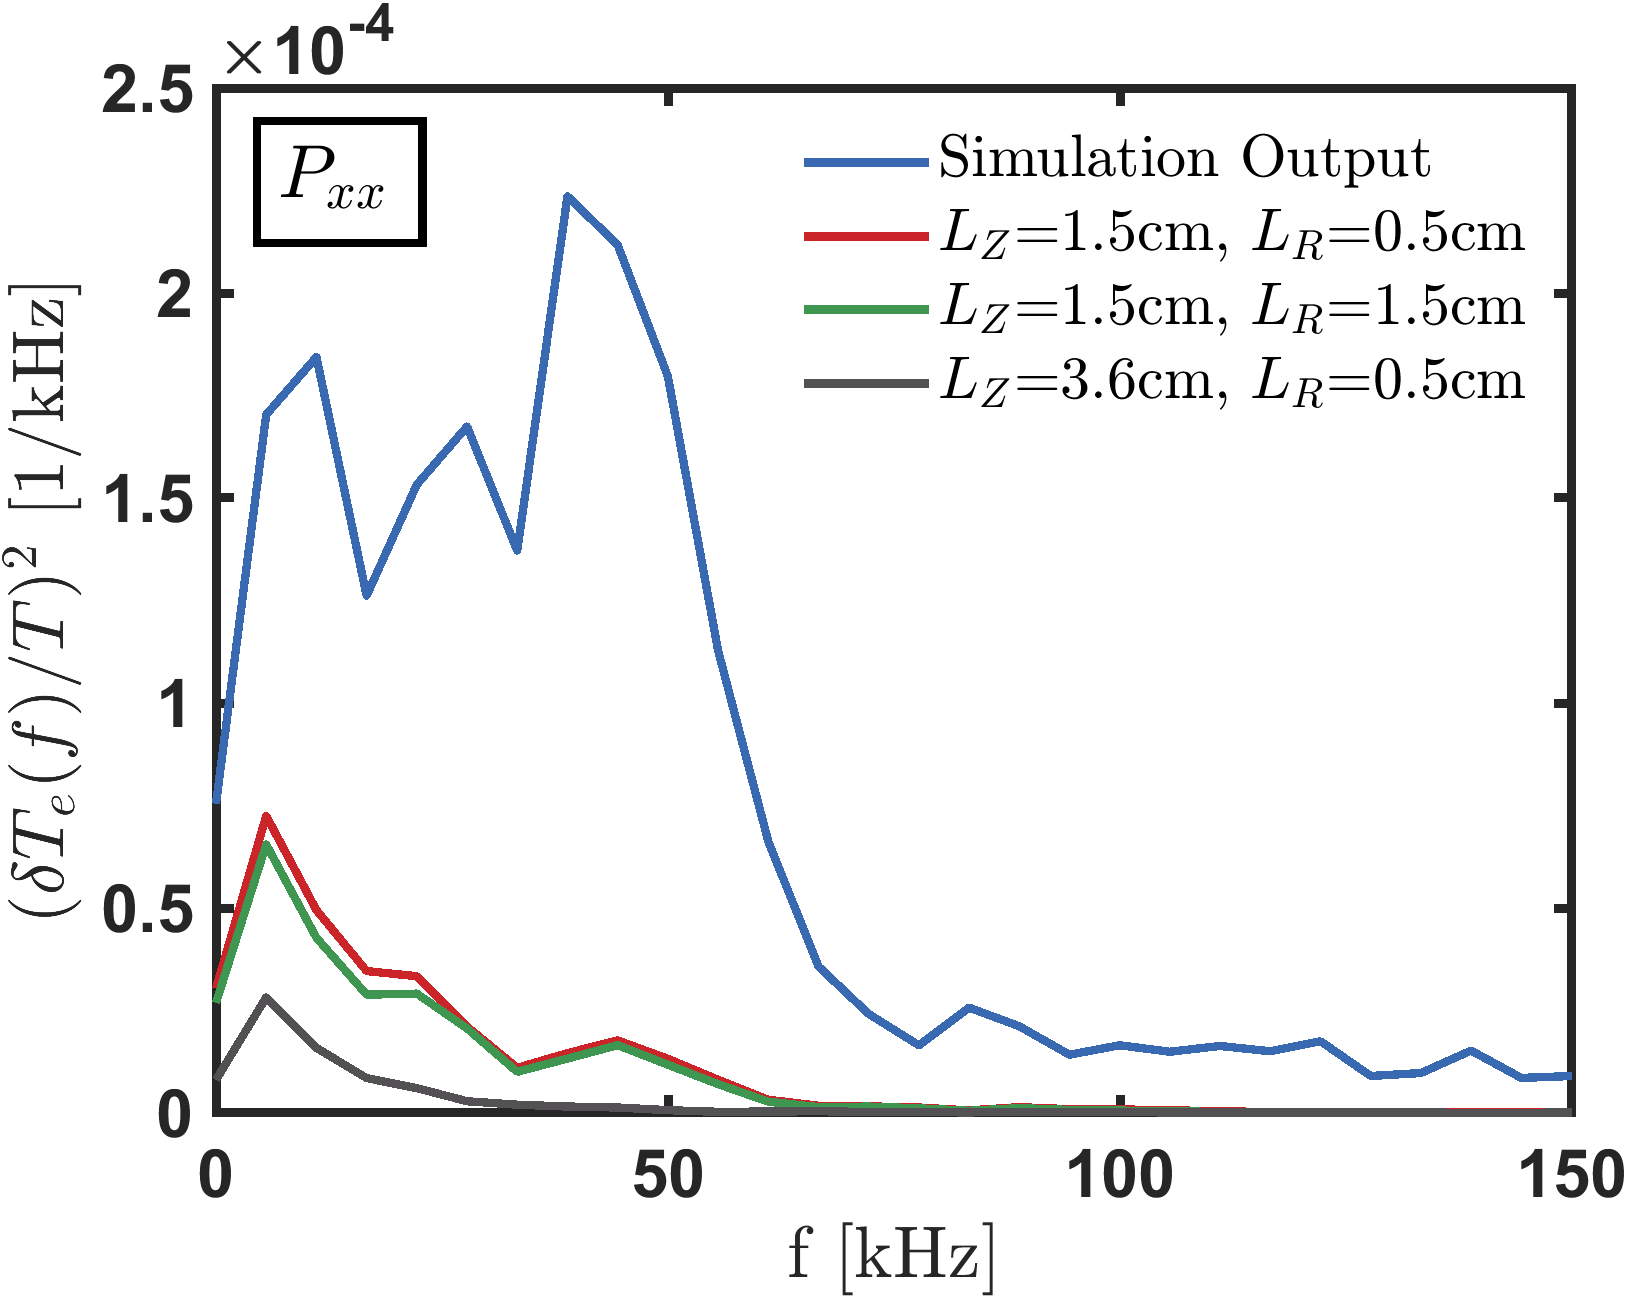
\includegraphics[width=\textwidth]{Figures/pxx_raw_vs_psf_a.png}}
\end{subfigure}
\hfill
\begin{subfigure}[]{.49\textwidth}
  \centering
  \subfloat[]{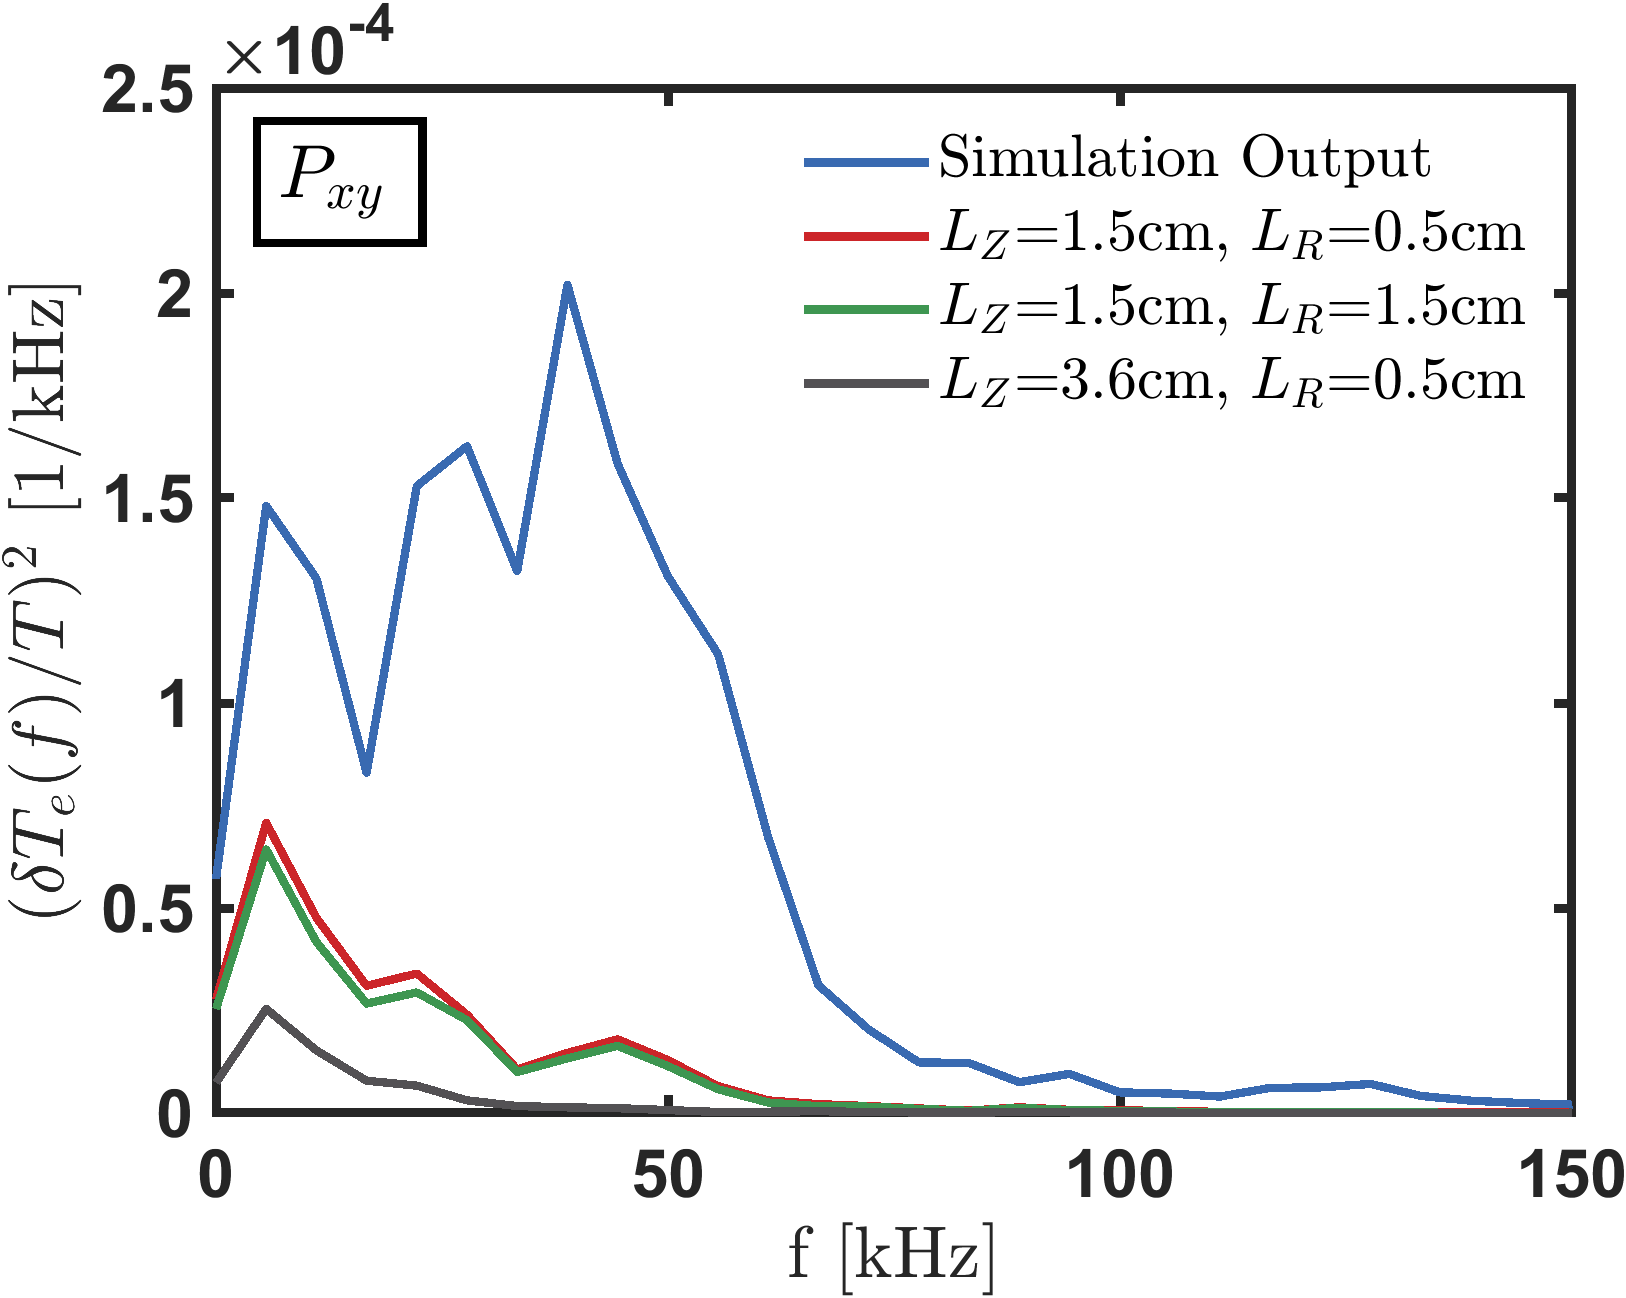
\includegraphics[width=\textwidth]{Figures/pxy_raw_vs_psf_a.png}}
\end{subfigure}
\hfill

\caption{Squared frequency spectrum of $\delta T_e/T_e$  corresponding to raw \gene{} output and ECE sample volume extents as determined by (a) the auto-power spectral density of a single synthetic ECE signal and (b) the cross-power spectral density of two synthetic ECE signals. The experimental parameters are $L_Z=1.5$\,cm and $L_R=0.5$\,cm.}
\label{fig:synth_sigs_unfilt_filt_spec}
\end{figure*}

% \begin{itemize}
% 	%\item Raw vs unfiltered shows way lower amplitude, attenuation of higher frequencies
% 	%\item This is a well-known result of wavenumber filtering
% 	%\item Attenuation in poloidal/toroidal directions preferentially tapers higher frequencies
% 	%\item Radial filtering tends to reduce spectrum at all frequencies
% \end{itemize}

For radial decorrelation CECE, the natural linewidth of emission is typically less than the ECE beam power radius, leading to $L_R<L_Z$. In HSX, $L_R \approx L_Z/3$, and consequently the shape of the temperature fluctuation spectrum is largely determined by the poloidal extent of the ECE sample volume. The spectrum of $\delta T_e/T_e$  corresponding to the time traces in Fig.\ \ref{fig:synth_sigs_unfilt_filt} and an additional synthetic signals with artificially high $L_Z$ and $L_R$ are shown in Fig.\ \ref{fig:synth_sigs_unfilt_filt_spec}. As reflected in the time traces, the spatially filtered synthetic signal corresponding to the experimental linewidth and beam radius is lower in amplitude as compared with the simulation output. Fig.\ \ref{fig:synth_sigs_unfilt_filt_spec}(a) shows that the majority of the spectral content is contained within approximately 100\,kHz for the simulation output, while the spectrum is largest within 50\,kHz for $L_z=1.5$\,cm and within 30\,kHz for $L_z=3.6$\,cm. This holds when considering the spectrum as computed using a single channel in Fig.\ \ref{fig:synth_sigs_unfilt_filt_spec}(b), implying that the simulated turbulence is similar within the ECE channel spacing in HSX; this is an underlying assumption of the CECE technique. In either case, increasing $L_Z$ leads to preferential attenuation of the fluctuation spectra at higher frequencies. The effect of tripling the experimental radial extent while holding the poloidal extent fixed is comparably negligible. This is consistent with the anticipated effect of finite sample volume on the frequency spectrum as described in \cite{ross1991dispersion,bravenec_wootton_spatial}.

\begin{figure*}[!htpb]
\centering
  {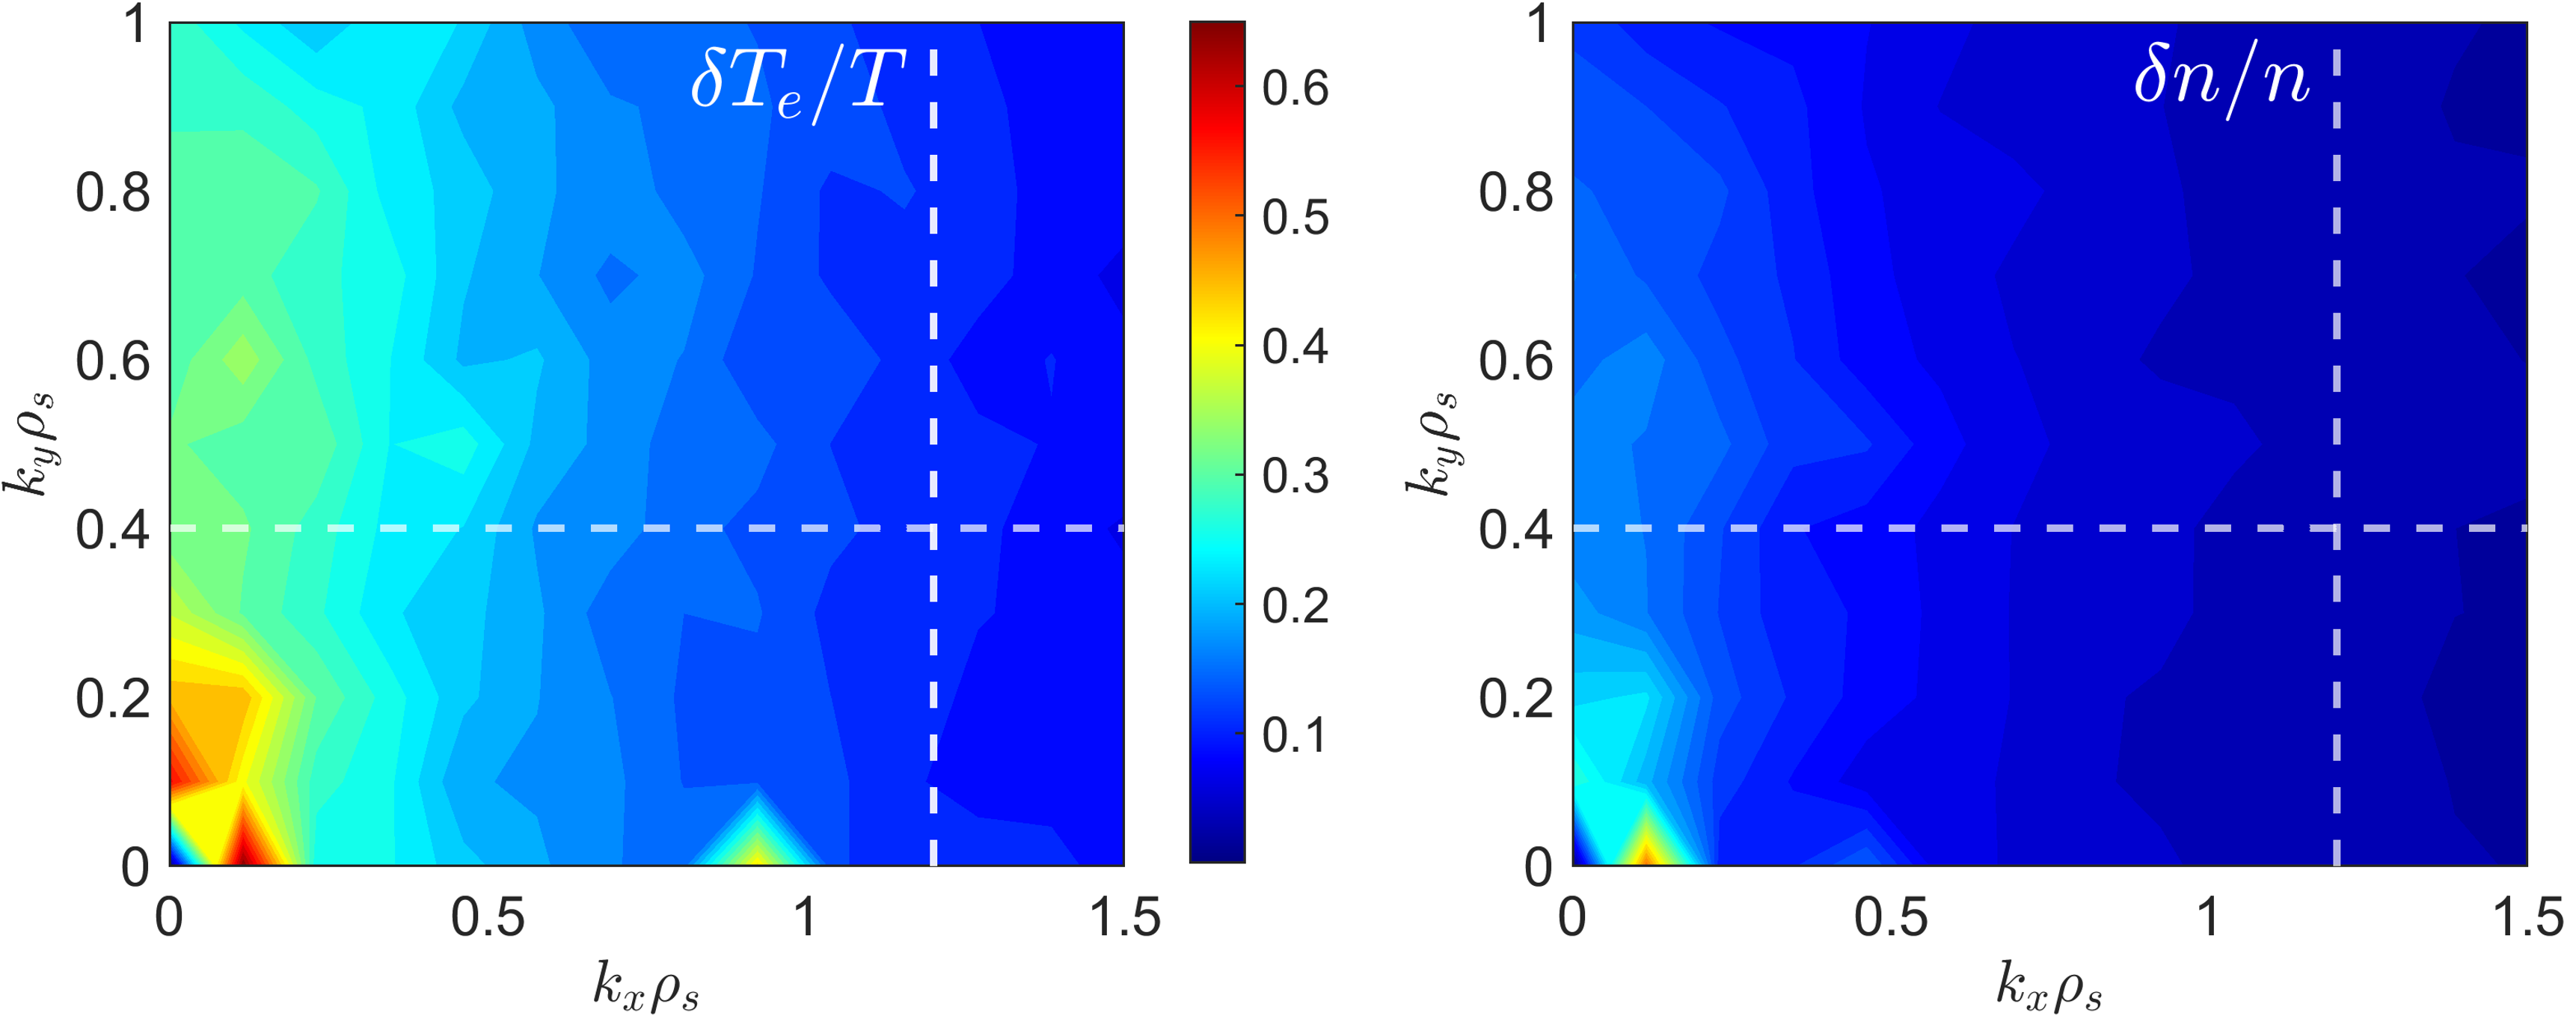
\includegraphics[width=\textwidth]{Figures/kxkycontour_omte4.png}}
\hfill
\caption{Normalized fluctuation amplitude spectra as a function of normalized wavenumber $k_x \rho_s$ and $k_y \rho_s$ for (left) electron temperature and (right) density. Dashed white lines indicate the approximate diagnostic sensitivity, with the bottom left quadrant corresponding to the range that CECE is primarily sensitive to. Coloring in both plots is equivalent. }
\label{fig:kxkyomte4}
\end{figure*}

To emphasize that it is primarily the poloidal extent of the channel defined by the ECE beamwidth that is responsible for the shape of the synthetic spectrum, contour plots of $\delta T_e/T_e$  and $\delta n/n$ are shown in Fig.\ \ref{fig:kxkyomte4} for a nonlinear simulation with $a/L_{Te}=6.5$, the frequency spectrum for which will be shown in Section \ref{sec:gk_omt_scan}. The approximate normalized wavenumber cutoff is indicated with dashed white lines, with the bottom left quadrant in each plot corresponding to the range that the CECE diagnostic is sensitive to. Little spectral content is present beyond the $k_x \rho_s$ bound (vertical line). On the other hand, the spectral content is significant above the $k_y \rho_s$ bound (horizontal line), particularly at low $k_x \rho_s$. This is true for both $\delta T_e/T_e$  and $\delta n/n$ but is more exaggerated for $\delta T_e/T_e$. Because the $k_y \rho_s$ bound filters out significantly more spectral content than the $k_x \rho_s$ bound, it is primarily $k_y \rho_s$ filtering that determines the synthetic (and experimental) spectrum.

% \subsubsection*{Synthetic Modeling of $\delta T_r/T_r$ }
Radiation temperature fluctuations are directly modeled using synthetic electron temperature and density fluctuation signals. The frequency spectrum of radiation temperature fluctuations is given by Eq.\ \eqref{eq:dTr_spectrum} and depends on plasma optical depth and vacuum vessel reflectivity, in addition to $\delta T_e/T_e$ and $\delta n/n$. This spectrum is integrated to derive a $\delta T_r/T_r$ fluctuation amplitude. The vessel reflectivity is taken as $\Gamma=0.9$, which is expected to be an underestimate in HSX. A near-unity vessel reflectivity would lead to $\delta T_r/T_r \approx \delta T_e/T_e$, so $\delta T_e/T_e$ is reported alongside $\delta T_r/T_r$ in all of the results shown. At low optical depth, the discrepancy between $\delta T_r/T_r$ increases if density and electron temperature fluctuations are in phase. Synthetic spectra corresponding to the integrated fluctuation amplitudes shown in Sections \ref{sec:gk_omn_scan} and \ref{sec:gk_omt_scan} can be found in Appendix \ref{app:D}. Due to device-size scale structures that are expected to affect turbulence saturation physics, the focus of the synthetic modeling in this chapter is on the shape of the $\delta T_r/T_r$ frequency spectrum and the scaling of integrated amplitudes with gradients, rather than on comparisons of exact values.


%%%%%%%%%%%%%%%%%%%%%%%%%%%%%%%%%%%%%%%%%%%%%%%%%%%%%%%%%%%%%%%%%%%%%%%%%%%%%%%%%%%%%%%%%%%%%%%%%%%%%%%%%%%%%%%%%%%%%%
% Below are the gradient scalings, which should probably be combined into one subsection, possibly one figure.
%%%%%%%%%%%%%%%%%%%%%%%%%%%%%%%%%%%%%%%%%%%%%%%%%%%%%%%%%%%%%%%%%%%%%%%%%%%%%%%%%%%%%%%%%%%%%%%%%%%%%%%%%%%%%%%%%%%%%%

\subsection{Density Gradient Scaling of $\delta T_r/T_r$ } \label{sec:gk_omn_scan}

Modeling the predicted scaling of radiation temperature fluctuations with driving gradients in the wavenumber range accessible to the CECE diagnostic is possible with nonlinear gyrokinetic simulations and a synthetic diagnostic. In this section, the dependence of $\delta T_r/T_r$  on the inverse scale length of the density gradient $a/L_n$ is investigated by first isolating the density gradient dependence at zero electron temperature gradient and then considering finite electron temperature gradient. Synthetic frequency spectra used to derive integrated fluctuation amplitudes in this chapter are shown in Appendix \ref{app:D}.

\begin{figure*}[!htbp]
\centering
\begin{subfigure}[]{.49\textwidth}
  \centering
  \subfloat[]{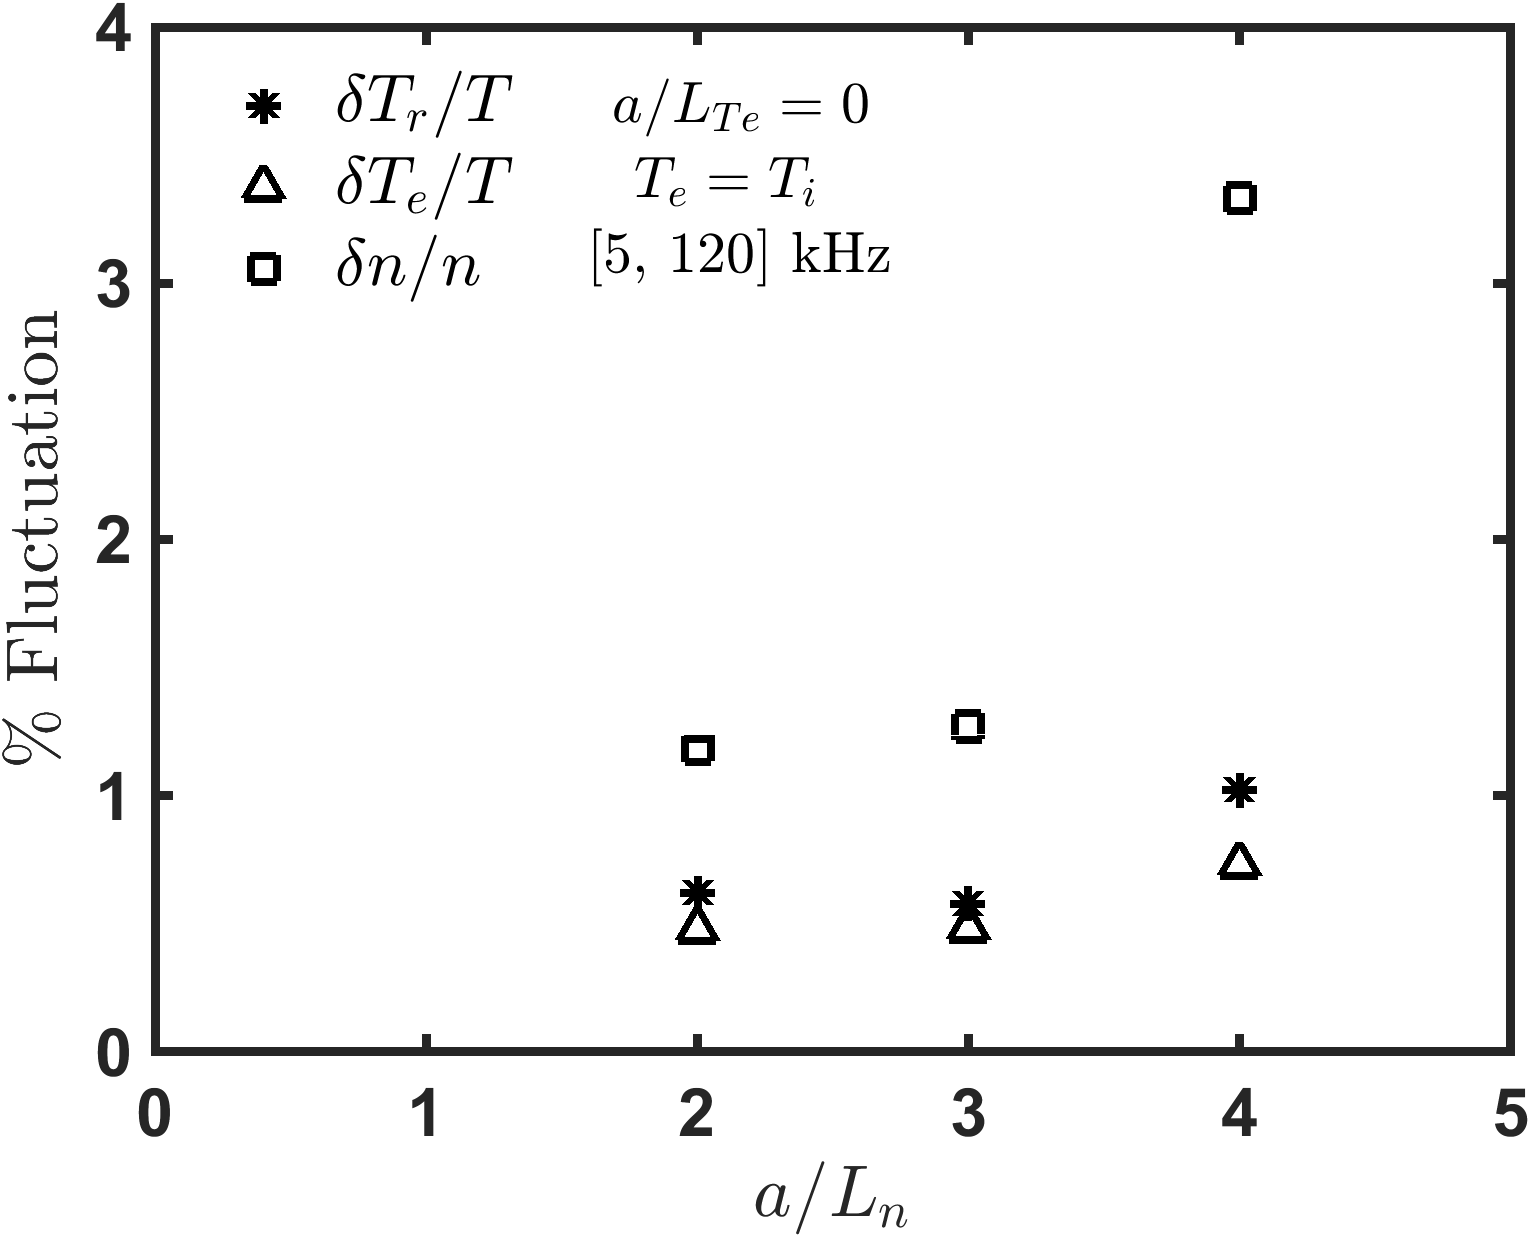
\includegraphics[width=\textwidth]{Figures/omne_fluc_summary.png}}
\end{subfigure}
\hfill
\begin{subfigure}[]{.49\textwidth}
  \centering
  \subfloat[]{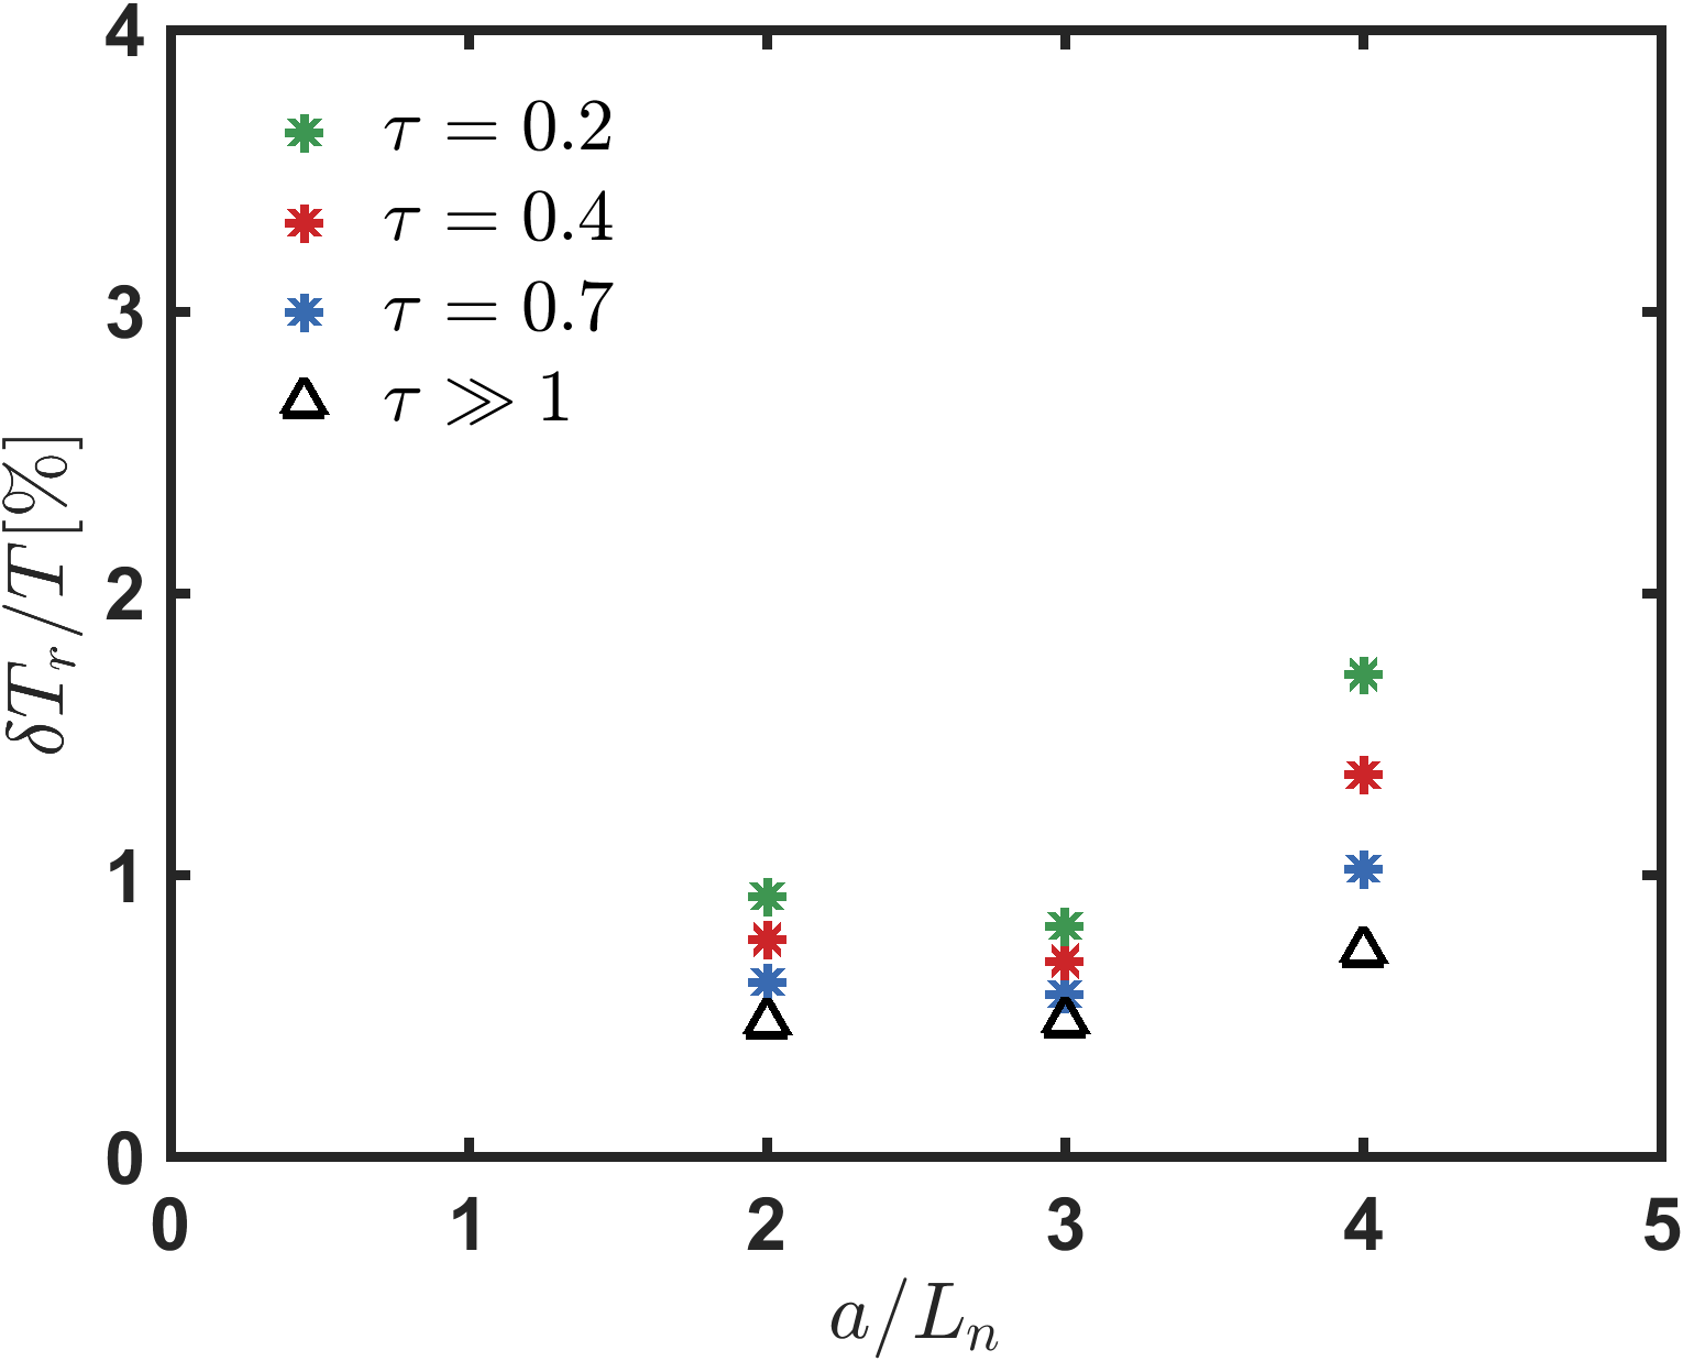
\includegraphics[width=\textwidth]{Figures/omne_a2.png}}
\end{subfigure}
\hfill
\caption{(a) Integrated fluctuation levels of electron temperature, density, and radiation temperature in the wavenumber range accessible to the HSX CECE diagnostic for a range of $a/L_n$ at zero $a/L_{Te}$. Fluctuations are integrated in the range of 5-120\,kHz. (b) Dependence of the radiation temperature fluctuation amplitude on optical depth assuming an effective vessel reflectivity of $\Gamma = 0.9$.}
\label{fig:omne_scan}
\end{figure*}


Fluctuation amplitudes $\delta T_r/T_r$  for $\tau=0.7$ and $\Gamma=0.9$ (see Eq.\ \eqref{eq:dTr_spectrum}), $\delta T_e/T_e$  and $\delta n/n$ are shown for simulations with three $a/L_n$ at zero $a/L_{Te}$ in Fig.\ \ref{fig:omne_scan}. The frequency spectra of $\delta T_e/T_e$  and $\delta n/n$ are integrated up to 120\,kHz because the data output rate of the simulation was limited in this series of simulations. This is not expected to significantly change the integrated values, as the fluctuation spectra are far higher in magnitude below 100\,kHz than beyond 100\,kHz. The fluctuation amplitude of all three quantities in Fig.\ \ref{fig:omne_scan} is approximately constant between the simulation at $a/L_n=2$ and $a/L_n=3$, and $\delta n/n$ is more than double $\delta T_e/T_e$. This holds at all relevant levels of optical depth, as shown in Fig.\ \ref{fig:omne_scan}(b). At $a/L_n=4$, the density fluctuation level triples compared to that at lower $a/L_n$, while $\delta T_e/T_e$  increases by less than a factor of two, and $\delta T_r/T_r$  corresponding to $\tau=0.7$ approximately doubles. A marginally higher increase in $\delta T_r/T_r$  from $a/L_n=3$ to $a/L_n=4$ is predicted at lower $\tau$, see Fig.\ \ref{fig:omne_scan}(b).


\subsection{Electron Temperature Gradient Scaling of $\delta T_r/T_r$ } \label{sec:gk_omt_scan}
CECE measurements show an increase in measured $\delta T_r/T_r$, as well as a likely increase in $\delta T_e/T_e$ with driving electron temperature gradient. In this section, nonlinear simulations scanning $a/L_{Te}$ at finite density gradient $a/L_n=2$ are presented, and the predicted scaling of $\delta T_r/T_r$  with $a/L_{Te}$ is compared with the database scaling in Section \ref{sec:dT_database}.

\begin{figure*}[!htbp]
\centering
\begin{subfigure}[]{.49\textwidth}
  \centering
  \subfloat[]{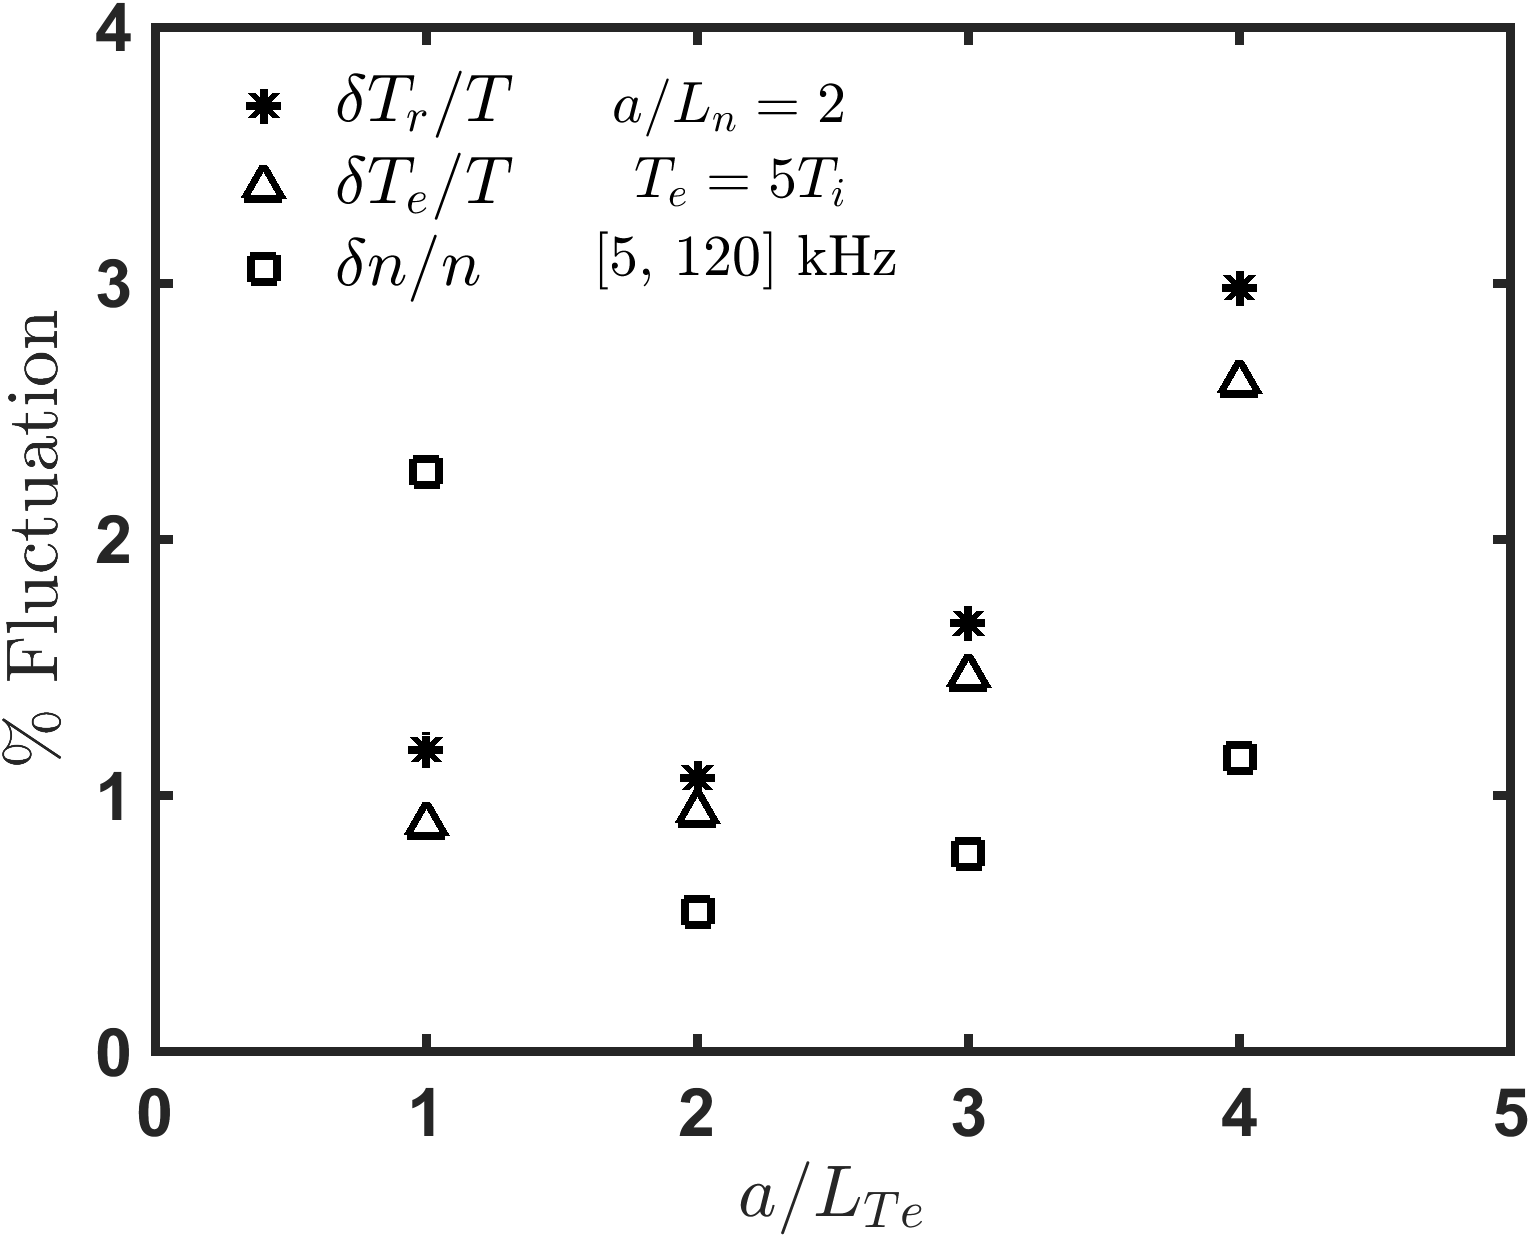
\includegraphics[width=\textwidth]{Figures/omte_fluc_summary.png}}
\end{subfigure}
\hfill
\begin{subfigure}[]{.49\textwidth}
  \centering
  \subfloat[]{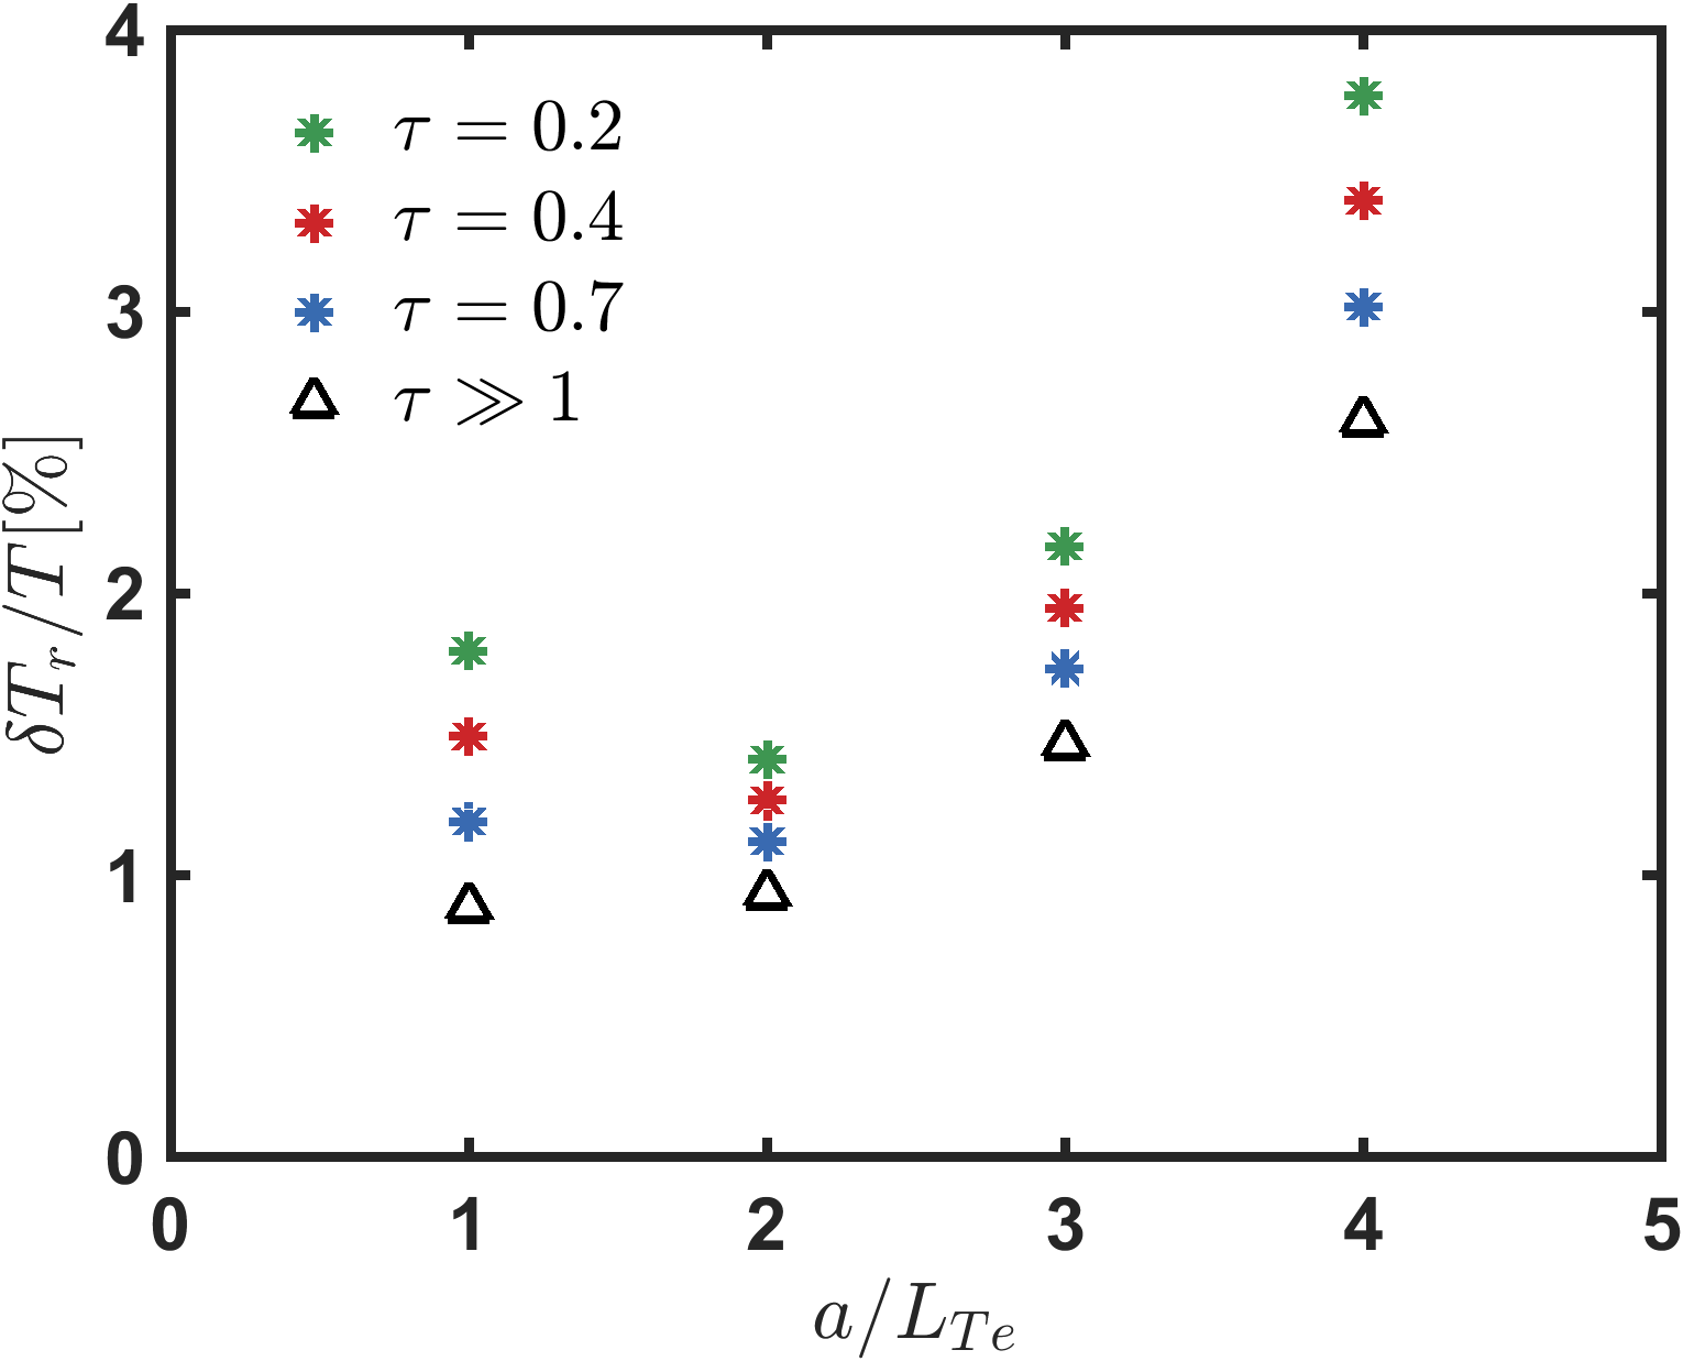
\includegraphics[width=\textwidth]{Figures/omte_a2.png}}
\end{subfigure}

\caption{Synthetic electron temperature, density, and radiation temperature fluctuations for four nonlinear \gene{} simulations scanning $a/L_{Te}$. The integrated fluctuation levels in the range of 5-120\,kHz are plotted in (a), and the dependence of $\delta T_r/T_r$  on optical depth assuming an effective vessel reflectivity of $\Gamma = 0.9$ is shown in (b). }
  \label{fig:omte_scan}
\end{figure*}

Fluctuation amplitudes $\delta T_r/T_r$  for $\tau=0.7$ and $\Gamma=0.9$, $\delta T_e/T_e$  and $\delta n/n$ are shown for simulations with three $a/L_{Te}$ and $a/L_{n}=2$ in Fig.\ \ref{fig:omte_scan}. The synthetic spectra are integrated up to 120\,kHz for consistency with those shown in Section \ref{sec:gk_omn_scan}. Fig.\ \ref{fig:omte_scan}(a) shows for $a/L_{Te}>2$ an increase in the fluctuation amplitude of all three fluctuating signals. In-phase density and temperature fluctuations lead to $\delta T_r /T_r > \delta T_e /T_e$ in each simulation, though the difference is moderate for $\tau=0.7$. $\delta T_r /T_r$ and $\delta T_e/T_e$  scale more strongly than $\delta n /n$ with $a/L_{Te}$, with $\delta T_e/T_e$  approximately tripling from $a/L_{Te}=2$ to $a/L_{Te}=4$ and $\delta n/n$ approximately doubling over the same range. Fig.\ \ref{fig:omte_scan}(b) shows that the scaling of $\delta T_r/T_r$  with $a/L_{Te}$ is not strongly dependent on optical depth. However, the magnitude of $\delta T_r/T_r$ increases significantly with decreasing optical depth. This is suggestive of in-phase density and electron temperature fluctuations. In the range of wavenumbers resolved by the CECE diagnostic, the cross-phases shown in Fig.\ \ref{fig:omt_crossphase} confirm that density and electron temperature fluctuations are primarily in phase at all values of $a/L_{Te}$.


%%%%%%%%%%%%%%%%%%%%%%%%%%%%%%%%%%%%%%%%%%%%%%%%%%%%%%%%%%%%%%%%%%%%%%%%%%%%%%%%%%%%%%%%%%%%%%%%%%%%%%%%%%%%%%%%%%%%%%
% Below are the comparisons of experiment and simulation, integrated and spectral.
%%%%%%%%%%%%%%%%%%%%%%%%%%%%%%%%%%%%%%%%%%%%%%%%%%%%%%%%%%%%%%%%%%%%%%%%%%%%%%%%%%%%%%%%%%%%%%%%%%%%%%%%%%%%%%%%%%%%%%

% Spectral comparison
\begin{figure*}[!htbp]
\begin{minipage}[]{\textwidth}
\center
\begin{subfigure}[]{.45\textwidth}
  	\subfloat[]{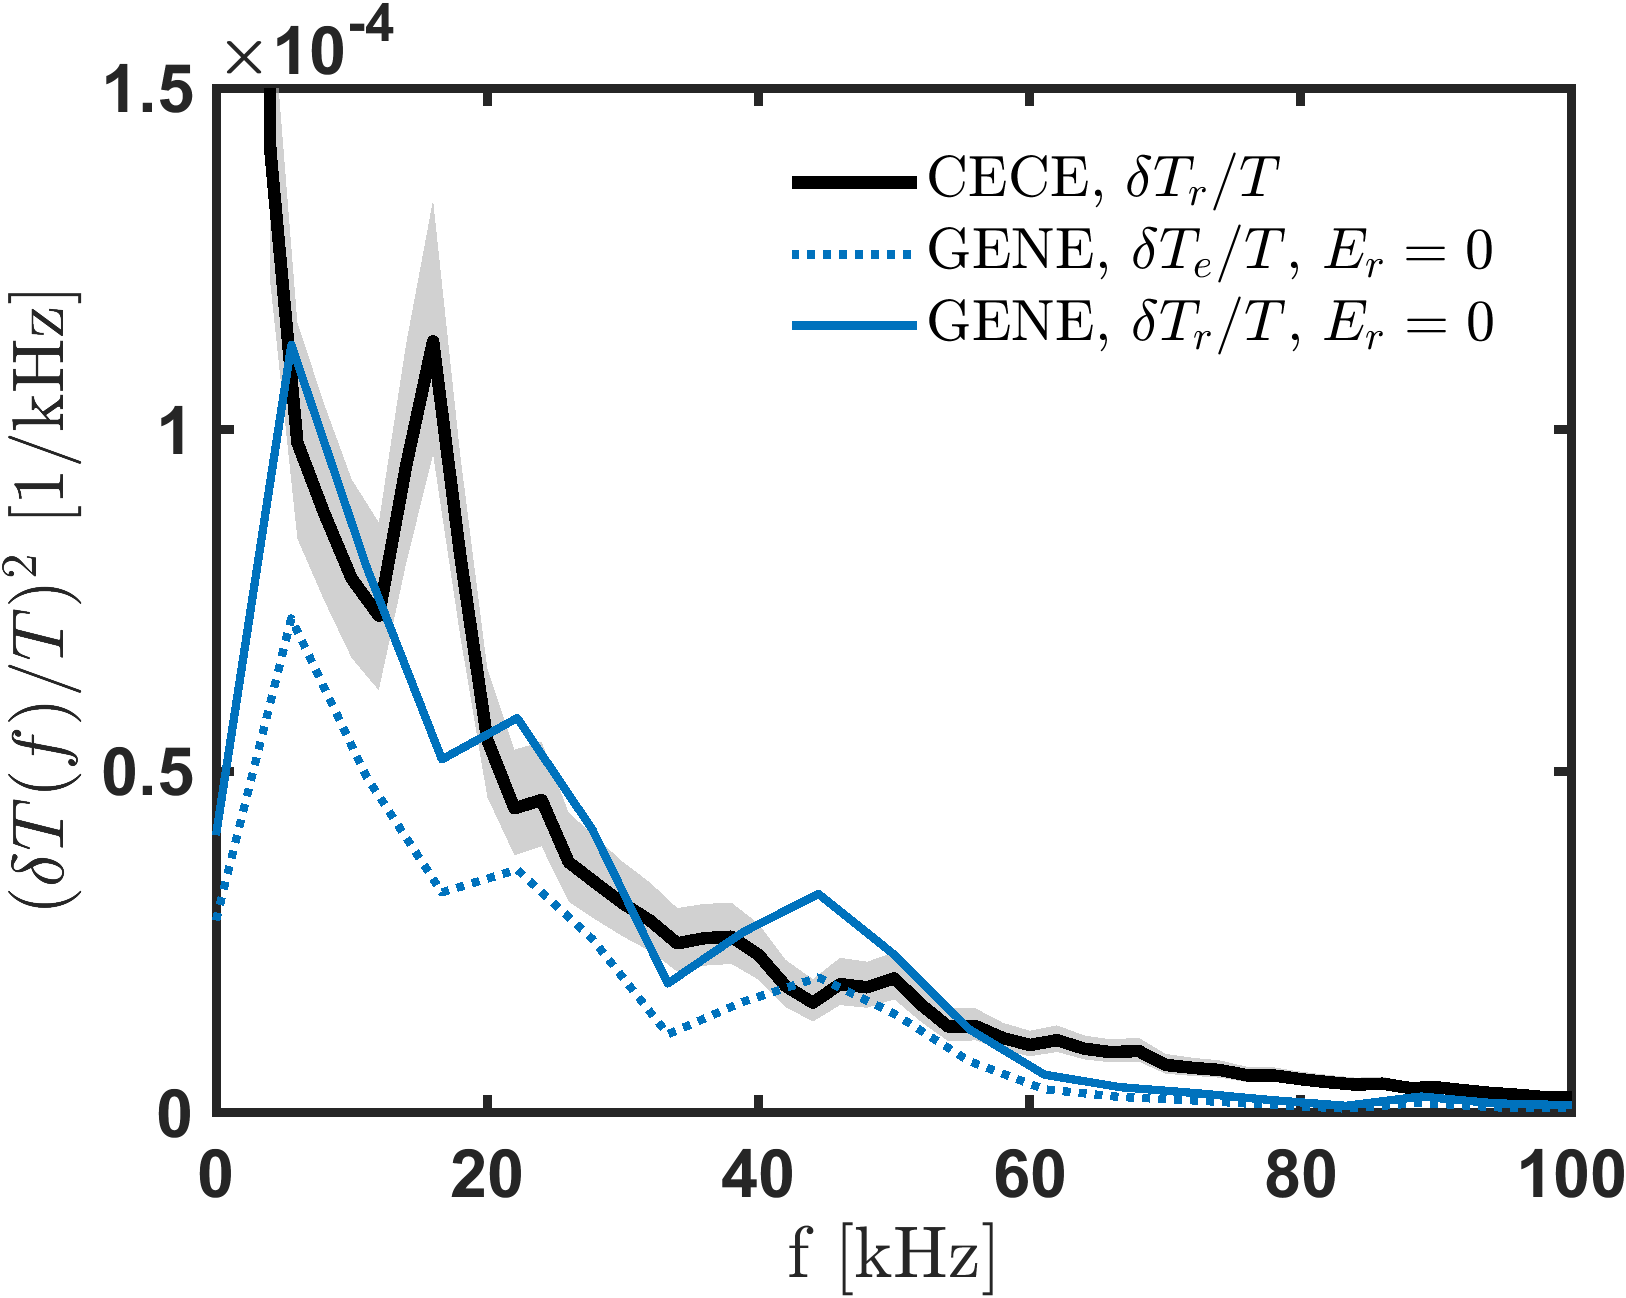
\includegraphics[width=\textwidth]{Figures/gene_vs_exp_linear.png}}
\end{subfigure}
\hfill
\begin{subfigure}[]{.45\textwidth}
  	\subfloat[]{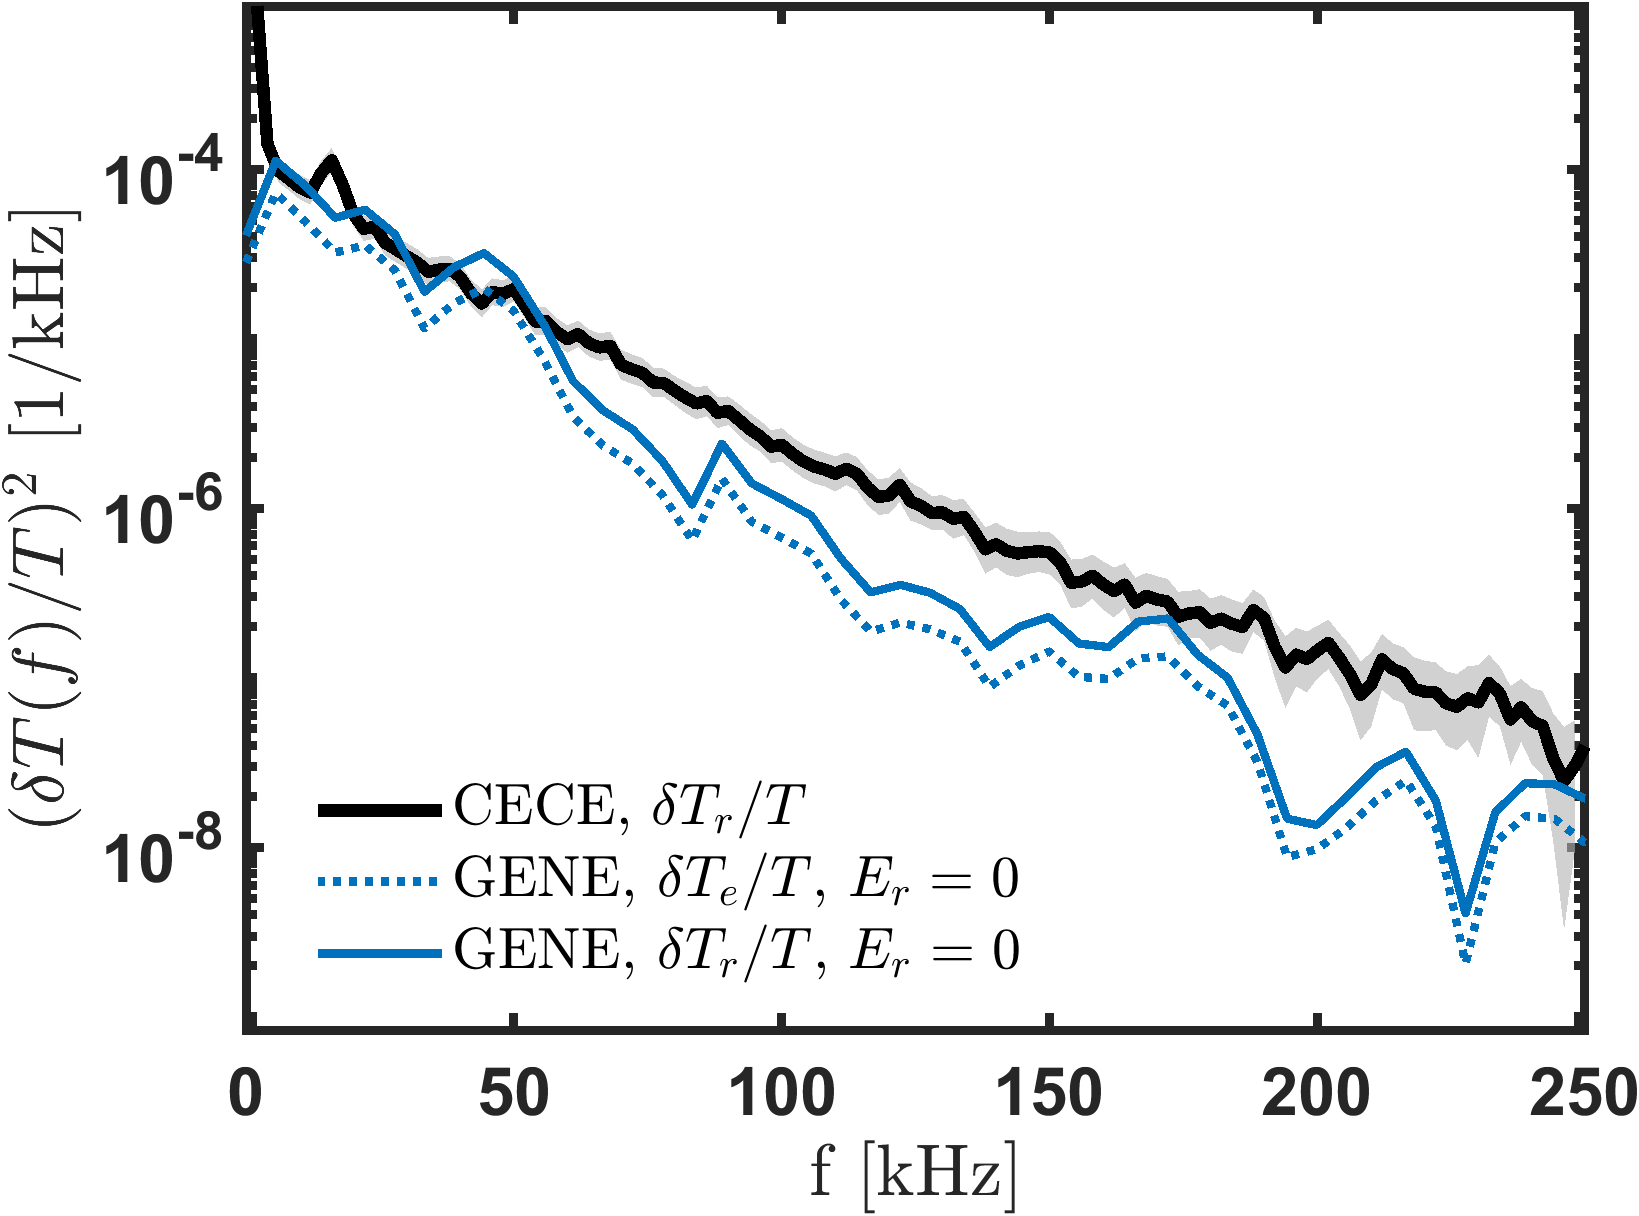
\includegraphics[width=\textwidth]{Figures/gene_vs_exp_log.png}}
\end{subfigure}

\captionof{figure}{Comparison of experimental and synthetic CECE (squared) fluctuation spectra. The spectra at frequencies below $f=100$\,kHz are shown on a linear scale in (a), and the same data is shown up to $f=250$\,kHz on a log-linear scale in (b). The synthetic $\delta T_r/T_r$ spectrum is computed using an optical depth $\tau=0.7$ and assuming an effective vessel reflectivity $\Gamma=0.9$. $\delta T_e/T_e$ here refers to the perpendicular component of electron temperature fluctuations. Corresponding integrated fluctuation levels are compared in multiple frequency bands in Table \ref{tab:exp_vs_gene}.}
  \label{fig:synth_exp_cmpr}
 
  \end{minipage}
 
\hfill
\vspace{.2cm}

\begin{minipage}[b]{.95\textwidth}
\begin{center}
\begin{tabular}{@{}ccccc@{}}
\toprule
\centering
Freq.\ Band & Exp.\ ($\delta T_r / T$) [\%] 	& Synth.\ ($\delta T_{r} / T$) [\%] & Synth.\ ($\delta T_{e} / T$) [\%] & Synth.\ ($\delta n / n$) [\%] \\ \midrule
{   }$5-200$\,kHz  & {$4.9 \pm 0.4$} & {4.60} & {3.83} & {1.77} \\
$20-200$\,kHz  	& {$4.3 \pm 0.3$} & {3.21} & {2.67} & {1.19} \\
$50-200$\,kHz  	& {$3.3 \pm 0.1$} & {1.23} & {1.02} & {0.61} \\ \bottomrule
\end{tabular}
\end{center}
\captionof{table}{Comparison of integrated $\delta T_r/T_r$  measured via CECE and predicted levels of $\delta T_{e} / T$ and $\delta T_{r} / T$  as determined using the \gene{} code coupled with a synthetic CECE diagnostic. The integrated values are computed using the spectra shown in Fig.\ \ref{fig:synth_exp_cmpr}.}
\label{tab:exp_vs_gene}
\end{minipage}
\end{figure*}

A nonlinear simulation has been performed at a high electron temperature gradient, $a/L_{Te}=6.5$, and processed with the synthetic diagnostic for comparison with an experimental CECE spectrum. The simulation input parameters and corresponding discharge parameters for the modeled discharge are shown in Table \ref{tab:sim_input_vs_exp}. Experimental parameters and uncertainties correspond with the base case introduced in Section \ref{sec:exp_cece}. There are moderate discrepancies in the values between the experimental discharge and simulation inputs. The base case discharge was identified from the database of CECE measurements in Section \ref{sec:dT_database} as the best match to the simulation inputs. In addition to the simulation inputs, the predicted turbulent transport and its agreement with the experiment are relevant to the comparison of the fluctuation spectrum. The saturated heat flux in gyroBohm units $Q_{GB}=c_s n_e T_e (\rho_s/a)^2$ is $Q_{e,es}/Q_{GB}\approx 10$ in this simulation. This exceeds the experimental level derived from multiple pass raytracing calculations of the power deposition profile using the base case plasma profiles, $Q_e^{exp}/Q_{GB}\approx1.4$.
Because the effect of a high heat flux on $\delta T_e/T_e$ is unclear ($Q_e$ depends on several additional quantities, see Eq.\ \eqref{eq:Qe_es}), this simulation data is suitable for a qualitative assessment of whether the measured spectrum is consistent with simulated low-wavenumber turbulence.    


The experimental $\delta T_r/T_r$ and synthetic $\delta T_r/T_r$  spectra are compared in Fig.\ \ref{fig:synth_exp_cmpr} with corresponding integrated values in three frequency ranges given in Table \ref{tab:exp_vs_gene}. The frequency spectrum of $\delta T_e/T_e$  is also shown, and it is clear that $\delta T_r/T > \delta T_e/T_e$  at all frequencies due to modification by density fluctuations, see Eq.\ \eqref{eq:dTr_spectrum}. The constituents of the $\delta T_r/T_r$  spectrum are shown in Fig.\ \ref{fig:nT_gk}(a) and an overlay of synthetic time traces of $\delta T_r/T_r$  and $\delta n/n$ is shown in Fig.\ \ref{fig:nT_gk}(b). To calculate $\delta T_r/T_r$, the average optical depth between both ECE channels used to generate the experimental spectrum is used is $\tau = 0.7$, and the $A_2$ factor in Eq.\ \eqref{eq:dTr_spectrum} is calculated assuming an effective vessel reflectivity $\Gamma=0.9$. From the signals shown in Fig.\ \ref{fig:nT_gk}(b), it is clear that density and electron temperature fluctuations are in phase, which is also reflected by positive values of the density-temperature cross-spectrum in  Fig.\ \ref{fig:nT_gk}(a).


Fig.\ \ref{fig:synth_exp_cmpr} shows there is an agreement between the measured and synthetic spectrum of $\delta T_r/T_r$, particularly below 50\,kHz. At higher frequencies, the experimental spectrum exceeds the predicted radiation temperature fluctuation spectrum. This is reflected in the integrated values in different signal bands; integration over the widest band leads to similar fluctuation amplitudes, while the signal amplitude in 50-200\,kHz is significantly higher in the experiment. The similarity of the experimental and synthetic spectrum provides evidence that TEM turbulence, which in this simulation is driven by the electron temperature gradient \cite{matthijs-msc}, can explain the appearance of the measured CECE spectrum. Resolving the aforementioned discrepancy in predicted heat flux will be required to better assess the predictive capability of flux-tube gyrokinetic simulations in HSX, which is beyond the scope of this work. A study of the sensitivity of the synthetic spectrum to changes in synthetic diagnostic inputs can be found in Appendix \ref{app:D}.


% Integrated comparison
\subsection{Comparison of Measured and Predicted Scaling of $\delta T_r/T_r$  with $a/L_{Te}$}

\begin{figure}[!htbp]
  \centering
  {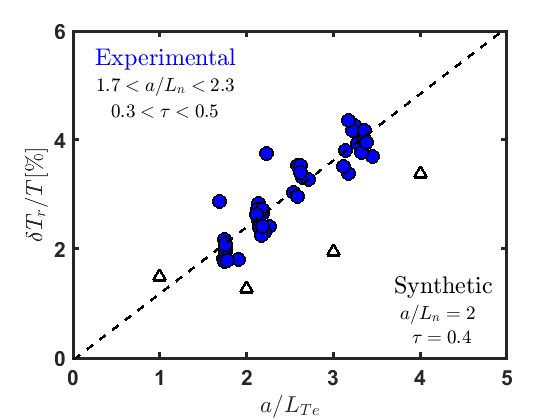
\includegraphics[width=.5\textwidth]{Figures/db_exp_vs_sim_final_line_nobar.png}}
\hfill

\caption{Overlay of the experimental database of $\delta T_r/T_r$ shown in Fig.\ \ref{fig:full_db}(c) with synthetic signals derived from the $a/L_{Te}$ scan simulations shown in Fig.\ \ref{fig:omte_scan}. The synthetic $\delta T_r/T_r$ are calculated using $\tau=0.4$, as this is the average optical depth over all the experimental measurements. The vessel reflectivity is taken as $\Gamma=0.9$. In contrast to the synthetic $\delta T_r/T_r$ shown in Fig.\ \ref{fig:omte_scan}, synthetic fluctuation amplitudes here reflect integration in 20-200\,kHz to be consistent with the experimental measurements. Representative vertical error bars are within the markers, while the horizontal error bar is approximately $\pm 1$.}
  \label{fig:omte_exp_synth}
\end{figure}


The trend in the nonlinear electron temperature gradient scan can be compared to that of $\delta T_r/T_r$ measured by CECE in HSX. This is shown in Fig.\ \ref{fig:omte_exp_synth}, where the integrated radiation temperature fluctuation amplitude in 20-200\,kHz from Fig.\ \ref{fig:full_db}(c) is plotted against the same result at $\tau=0.4$ result in Fig.\ \ref{fig:omte_scan}(b) but in the range of 20-200\,kHz (this change in frequency bounds has little effect on the fluctuation amplitude and was chosen for consistency with the experimental analysis settings). For this comparison, $\tau=0.4$ is chosen because this is the average optical depth of all experimental measurements shown. For the range of $T_e$ in the experimental database, the upper bound on the wavenumber sensitivity is $0.35 < k_y \rho_s <0.42$, and the $L_Z$ value used in the synthetic diagnostic corresponds with $k_y \rho_s = 0.4$. For these simulations, the saturated heat flux is in the range 1.5-2.5\,$Q_{GB}$, which is within a factor of 2 of the experimental heat fluxes.  

The trend of increasing $\delta T_r/T_r$ with $a/L_{Te}>2$ in the experiment is in agreement with synthetic data. However, the measured fluctuation amplitude is higher than the synthetic. It is noteworthy that the trend in Fig.\ \ref{fig:omte_scan}(b) is well-expressed even for $\tau \gg 1$, corresponding to $\delta T_e/T= \delta T_r/T_r$. Agreement in this trend indicates that local gyrokinetic simulations can predict the behavior of experimental fluctuation amplitudes in optimized stellarators. Given that $a/L_{Te}>a/L_n$ in the simulations best matched to the experimental conditions, this agreement provides further evidence that CECE is sensitive to electron-temperature-gradient-driven TEMs.






\section{\label{sec:conclusion}Conclusions}


\begin{acknowledgments}
We wish to acknowledge the support of the author community in using
REV\TeX{}, offering suggestions and encouragement, testing new versions,
\dots.
\end{acknowledgments}

\section*{Data Availability Statement}
The data that support the findings of this study are available from the
corresponding author upon reasonable request.

\appendix

%\section{Appendixes}

%\nocite{*}
\bibliographystyle{aipnum4-1}
\bibliography{refs}% Produces the bibliography via BibTeX.

\end{document}
%
% ****** End of file aipsamp.tex ******